\documentclass{ieeeaccess}
\usepackage{cite}
\usepackage{amsmath,amssymb,amsfonts}
\usepackage{algorithmic}
\usepackage{graphicx}
% Figures and the IEEE Access logos live one level up (shared across the
% per-document folders); this makes \includegraphics{Figures/...} and the
% class logos resolve from the parent directory.
\graphicspath{{../}}
\usepackage{textcomp}
\usepackage{makecell}
\usepackage{booktabs}
\usepackage{float}
\usepackage{subcaption}
\usepackage{xcolor}
\usepackage{hyperref}
\usepackage{varioref}
\usepackage{cleveref}
% Reference names in IEEE style: "Fig. 3", "Table 5", "Section IV-B", "(1)".
\crefname{figure}{Fig.}{Figs.}
\Crefname{figure}{Fig.}{Figs.}
\crefname{table}{Table}{Tables}
\Crefname{table}{Table}{Tables}
\crefname{section}{Section}{Sections}
\Crefname{section}{Section}{Sections}
\crefname{subsection}{Section}{Sections}
\Crefname{subsection}{Section}{Sections}
\crefformat{equation}{(#2#1#3)}
\Crefformat{equation}{(#2#1#3)}
% Reference names in IEEE style: "Fig. 3", "Table 5", "Section IV-B", "(1)".
\crefname{figure}{Fig.}{Figs.}
\Crefname{figure}{Fig.}{Figs.}
\crefname{table}{Table}{Tables}
\Crefname{table}{Table}{Tables}
\crefname{section}{Section}{Sections}
\Crefname{section}{Section}{Sections}
\crefname{subsection}{Section}{Sections}
\Crefname{subsection}{Section}{Sections}
\crefformat{equation}{(#2#1#3)}
\Crefformat{equation}{(#2#1#3)}
\hypersetup{colorlinks=true,linkcolor=black,citecolor=black,urlcolor=black}

% Improved float placement settings
\setlength{\textfloatsep}{10pt plus 2pt minus 2pt}
\setlength{\intextsep}{10pt plus 2pt minus 2pt}
\setlength{\floatsep}{10pt plus 2pt minus 2pt}

% Allow more floats per page
\renewcommand{\topfraction}{0.9}
\renewcommand{\bottomfraction}{0.8}
\renewcommand{\textfraction}{0.1}
\renewcommand{\floatpagefraction}{0.8}
\setcounter{topnumber}{3}
\setcounter{bottomnumber}{3}
\setcounter{totalnumber}{5}

\def\BibTeX{{\rm B\kern-.05em{\sc i\kern-.025em b}\kern-.08em
    T\kern-.1667em\lower.7ex\hbox{E}\kern-.125emX}}
\begin{document}
\history{Date of publication xxxx 00, 0000, date of current version xxxx 00, 0000.}
\doi{10.1109/ACCESS.2017.DOI}

\title{Deep Reinforcement Learning with Runtime Safety Monitoring for Cartesian Path Tracking of Free-Floating Space Robot Manipulators: A Benchmark}
\author{\uppercase{Patrick S. Ermisch}\authorrefmark{1}, and 
\uppercase{Eric Guiffo Kaigom\authorrefmark{1}} }
\address[1]{Department of Computer Science \& Engineering, Frankfurt University of Applied Sciences,
Frankfurt am Main, Germany \\(e-mail: steven.ermisch@stud.fra-uas.de, kaigom@fra-uas.de)}
%\address[2]{Department of Physics, Colorado State University, Fort Collins, 
%CO 80523 USA (e-mail: author@lamar.colostate.edu)
%}
%\tfootnote{This paragraph of the first footnote will contain support  information, including sponsor and financial support acknowledgment. For example, ``This work was supported in part by the U.S. Department of Commerce under Grant BS123456.''}

\markboth
{P. S. Ermisch and E. G. Kaigom: Deep RL with Runtime Safety Monitoring for Free-Floating Space Manipulators}
{P. S. Ermisch and E. G. Kaigom: Deep RL with Runtime Safety Monitoring for Free-Floating Space Manipulators}

\corresp{Corresponding author: Eric Guiffo Kaigom (e-mail: kaigom@fra-uas.de).}

\begin{abstract}
The base reaction of free-floating space robots (FFSRs) complicates Cartesian path tracking of their
end-effector. On-orbit data are scarce, making simulation-based control policy training through
interaction and task-specific rewards attractive. This work benchmarks six deep reinforcement learning
algorithms (TRPO, TD3, SAC, PPO, PG, and DDPG) for planar Cartesian path tracking of an FFSR in a
physics-based Simulink/Simscape environment with runtime safety monitoring. Each configuration is
trained with ten seeds. Success rate and performance of successful runs are evaluated separately with
unified metrics. With default hyperparameters, only TRPO completes all ten runs without a safety abort
caused by a monitored collision or joint-limit violation, whereas other agents terminate 40\% to 80\% of
their evaluation episodes. Even in their successful runs, SAC, DDPG, and TD3 track the path with a
significantly larger error than TRPO. A tuned PPO configuration also completes all runs and reaches the
lowest mean squared tracking error (0.0041 compared with 0.0145 for TRPO) in less training time, but
this difference is not statistically significant. On a piecewise-linear path, its tracking error is
again lower than that of TRPO, but not significantly after a multiple-comparison correction. Both
agents complete all runs under observation noise, reduced torque limits, an external joint torque, and
masses, inertias, and joint damping uniformly increased by 50\%. All results are simulation-based under
controlled assumptions and do not establish operational readiness. The safety component comprises
runtime monitors for selected properties and a formal check of torque saturation, but is not a formal
proof of closed-loop safety.
\end{abstract}
\begin{keywords}
Free-floating on-orbit servicing, Proximal Policy Optimization (PPO), reinforcement learning,
safety monitoring, space robotics, trajectory tracking, extended agentic systems intelligence (EASI)
\end{keywords}

\titlepgskip=-15pt

\maketitle

\section{Introduction and Background}

\begin{figure}[!t]
	\centering
	\begin{subfigure}{0.99\columnwidth}
		\centering
		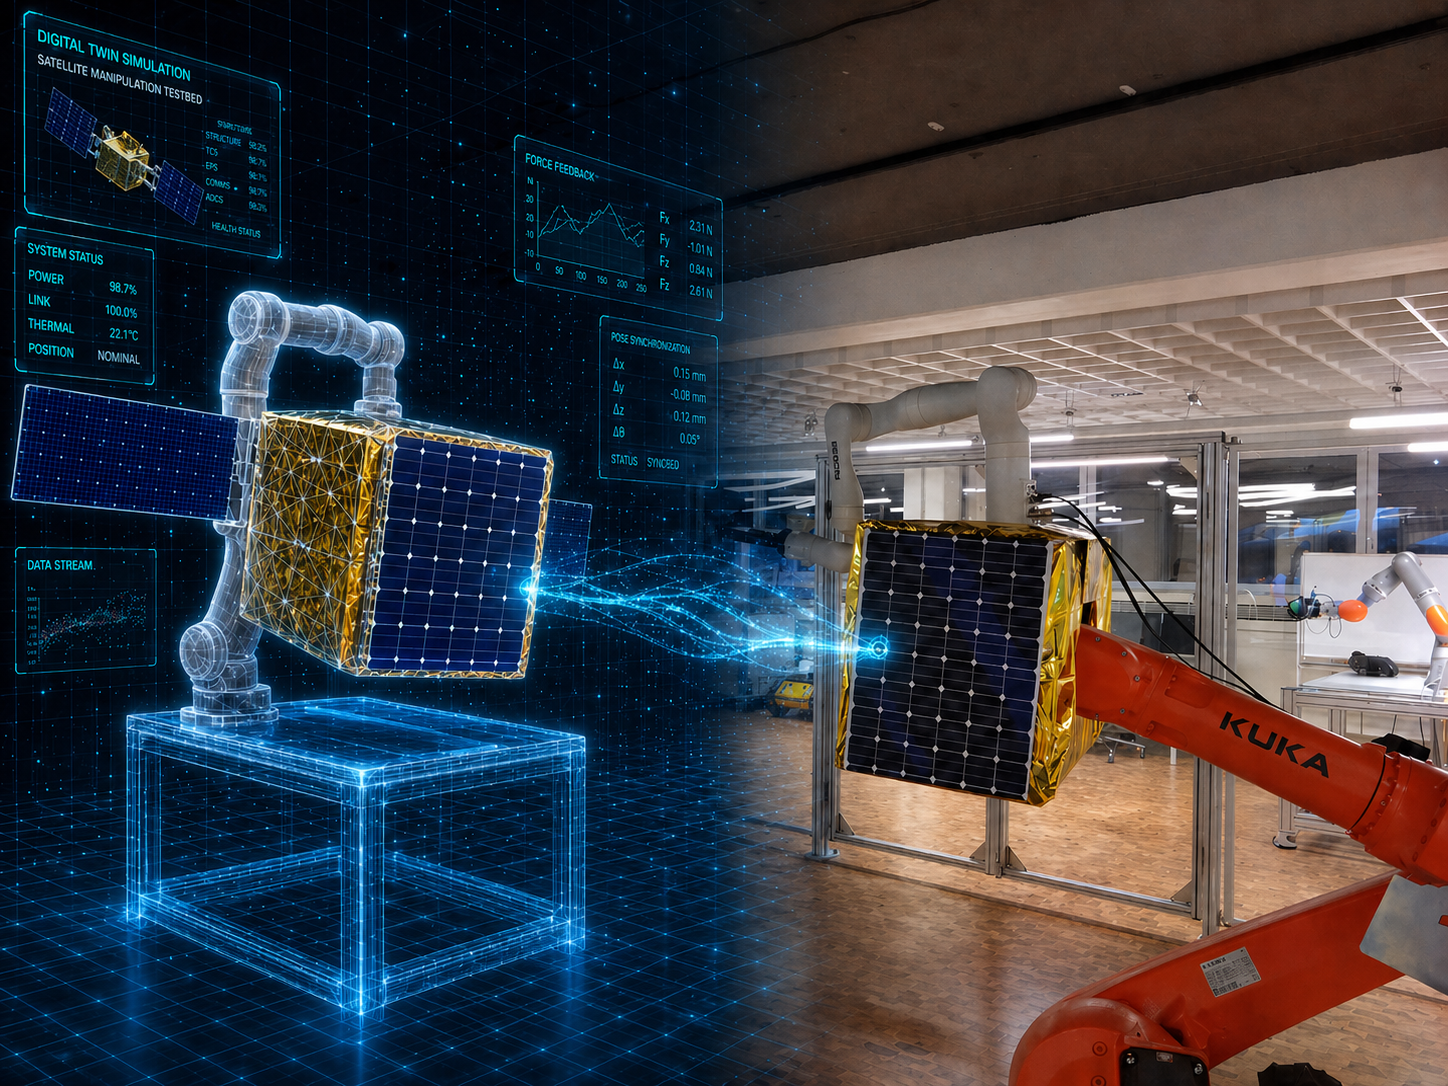
\includegraphics[width=\linewidth]{Figures/oos1.png}
	\end{subfigure}
	\caption{Concept of a hybrid testbed for in-space robotic services. An AI-driven digital twin (left) is
	linked to the physical setup (right). This work covers only the simulation side, and the physical setup
	is intended for future sim-to-real studies. Illustration created with GPT-Image-2 from a photograph of
	the physical setup.}
	\label{fig:oos}
\end{figure}

Free-floating robot manipulators operating in space for satellite inspection, capture, or de-orbiting 
introduce control challenges not encountered with terrestrial robots \cite{b1}.
In microgravity, the robot's base (typically a spacecraft) is not fixed, and the thrusters
are inactive.
Manipulator motions therefore change the position and orientation of the base, which in turn
modifies the 
pose of the end-effector. This reaction is a consequence of the conservation of
linear and angular momentum \cite{b6}. Operating the manipulator under free-floating dynamics avoids the 
consumption of propellant (e.g., hydrazine, $\mathrm{N_2H_4}$) and the excitation of structural modes by 
the pulse-width modulation of thruster control at certain frequencies \cite{b11}. This can extend the operational
lifetime of the spacecraft.


However, a free-floating base complicates manipulator control.
Standard motion-planning approaches developed for fixed-base robots can fail to drive the end-effector to 
the desired target. Additional constraints, such as communication latency
and limited onboard computational resources, further complicate continuous real-time control and base 
stabilization \cite{b1,b32}. Model-based approaches that assume an accurate dynamic model (e.g., reactionless 
planning or precise attitude control)
are sensitive to model uncertainty and unmodeled dynamics. Supervised data-driven approaches are also 
difficult to apply because
labeled training data of sufficient amount and quality are typically unavailable in the space
sector.
In addition, tracking capability under a free-floating base often has to be
demonstrated before the physical system is assembled and deployed 
\cite{muhlbauer2025software,rybus2024robotic,kaigom2011optimal}.


These challenges motivate the development and simulation of AI-enabled digital twins (DTs)
\cite{kaigom2025deep,la2025deep}, as illustrated in \cref{fig:oos}. Unlike standard DTs that primarily mirror sensed
real-time data from physical counterparts, AI-enabled DTs combine physics-based simulation with learning
components to contextualize system states and evaluate representative operating conditions. Such conditions
can include uncertain dynamics, disturbances, faults, and contact-rich interactions associated with
satellite capture. Faster-than-real-time simulation and systematic ablation studies can support controller
design and help assess sim-to-real effects. In this role, AI-enabled DTs can provide a training and
validation environment for learning-based controllers, in particular when flight data are limited and the
constraints are safety-critical. The DT in this work covers only the space robot under nominal
free-floating conditions (see \cref{sec:sim}).



\begin{table*}[!t]
	\centering
	\caption{Recent advances in deep RL-based motion management for free-floating space robots.
  Abbreviations: RL Alg.\,=\,reinforcement learning algorithm; DOF\,=\,degrees of freedom;
  Obs./Act.\,Dim.\,=\,observation-/action-space dimension; vel.\,=\,joint velocities; rates\,=\,joint
  rate commands; pos./att.\,=\,position/attitude; pos./ori.\,=\,position/orientation;
  EE\,=\,end-effector; Formal Meth.\,=\,formal verification of safety properties; Base Dist.\,Min.\,=\,base
  disturbance minimization; $d_{\mathrm{safe}}$\,=\,minimum admissible distance; $\tau_{\max}$\,=\,torque
  bound; $K_1$--$K_9$\,=\,evaluation KPIs (see \cref{RL}); N/R\,=\,not reported; $^{\dagger}$only the
  torque bound of the actuation path is formally checked, collisions and joint limits are monitored at
  runtime, and the closed loop is not formally verified.}
	\label{tab:sample}
	\scriptsize
	\renewcommand{\arraystretch}{1.25}
	\begin{tabular}{lcccccccc}
		\toprule
		\textbf{Contribution} & \makecell{\textbf{RL}\\\textbf{Alg.}} & \textbf{Task Objective} &
		  \textbf{DOF} & \textbf{Simulator} & \makecell{\textbf{Obs./Act.}\\\textbf{Dim.}} &
		  \makecell{\textbf{Safety}\\\textbf{Limits}} & \makecell{\textbf{Eval.}\\\textbf{Metrics}} &
		  \makecell{\textbf{Formal Meth./}\\\textbf{Base Dist. Min.}} \\
		\midrule
		\cite{huang2023obstacle}, 2023 & SAC & Obstacle avoidance & 7 & OpenAI Gym & 14\,/\,7D vel. &
		  Reward-based & Success rate & No/No \\
		\cite{al2024reinforcement}, 2024 & DDPG & Collision avoidance & 6 & Custom & N/R\,/\,6D vel. &
		  Reward-based & Success rate & No/No \\
		\cite{d2024failure}, 2024 & PPO & \makecell{Joint failure\\adaptation} & 7 &
		  \makecell{MATLAB\\Simscape + SPART} & 32\,/\,7D rates & \makecell{Pos./att.\\threshold} &
		  \makecell{Per-joint\\success rate} & No/No \\
		\cite{al2024path}, 2024 & DDPG & Path planning & 6 & Custom & 32\,/\,6D vel. & Reward-based &
		  \makecell{Convergence,\\task completion} & No/No \\
		\cite{hu2025deep}, 2025 & PPO & Trajectory planning & 6 & PyBullet & N/R\,/\,6D & Joint limits &
		  \makecell{Success rate,\\pos./ori. error} & No/No \\
		\cite{zhang2025learning}, 2025 & LSAC & \makecell{Trajectory\\post-processing} & N/R &
		  \makecell{Custom +\\air-bearing} & N/R\,/\,N/R & \makecell{Uncertainty\\bounds} & Tracking error &
		  No/No \\
		\cite{wei2025trajectory}, 2025 & DDPG & Trajectory planning & N/R & Custom & N/R\,/\,N/R &
		  \makecell{Base dist.\\(soft)} & \makecell{Reward,\\base dist. red.} & No/Yes \\
		\midrule
		\textbf{This work} & \makecell{\textbf{PG, PPO,}\\\textbf{TRPO, DDPG,}\\\textbf{TD3, SAC}} &
		  \makecell{\textbf{Cartesian EE}\\\textbf{tracking}} & \textbf{4} &
		  \makecell{\textbf{MATLAB/Simulink}\\\textbf{+ Simscape}} & \textbf{23\,/\,4D} $\boldsymbol{\tau}$ &
		  \makecell{$d_{\mathrm{safe}}$, $\tau_{\max}$,\\joint limits} & $K_1$--$K_9$ &
		  \textbf{Partial}$^{\dagger}$\textbf{/Yes} \\
		\bottomrule
	\end{tabular}
\end{table*}

Reinforcement learning (RL) has been increasingly applied in robotics. An RL agent learns a control policy
through trial-and-error interaction with its environment. Recent advances in deep RL
have addressed a range of complex continuous-control tasks, although applications to space robots remain
comparatively recent \cite{wu2020reinforcement,al2024path,hu2025deep,zhang2025learning,huang2023obstacle}.

This work investigates continuous-action deep RL for Cartesian path tracking of the end-effector of
a free-floating space
manipulator. The contribution differs from prior work in three respects. First, six RL algorithms are compared
under the same conditions (see \cref{comparison}), complemented by ablation studies (see \cref{sec:reward_ablation}).
The works listed in \cref{tab:sample} do not provide such a comparison. Second, collisions and joint limits
are monitored at runtime in the training and evaluation loop, and the torque bound of the actuation path is
checked formally (see \cref{formal}). Third, base attitude minimization during arm motion is treated as an
explicit control objective in conjunction with the constraint monitoring above. The induced base
disturbance is not addressed in most of the works listed in \cref{tab:sample}. To the authors' knowledge,
a unified comparison of RL algorithms for Cartesian path tracking of free-floating space robots that
jointly considers base attitude minimization and runtime constraint monitoring remains unavailable.

As shown in \cref{tab:sample}, the surveyed prior contributions typically evaluate a single RL algorithm
on a specific subtask, which limits conclusions about the relative merits of different learning
algorithms for free-floating space robot control. In addition, the surveyed works do not combine three
aspects. These are (i)~a multi-algorithm benchmark under unified conditions, (ii)~explicit minimization
of the base attitude disturbance alongside end-effector tracking, and (iii)~runtime safety monitoring in
the RL training and evaluation loop. This work addresses these aspects together in a reproducible
simulation benchmark with runtime monitoring of selected safety properties, which extends the individual
studies listed in \cref{tab:sample}.

The main contributions of this work are summarized as follows:

\begin{itemize}
  \item \textit{Comparative evaluation of RL agents.} Six continuous-action RL algorithms are implemented
  and evaluated on the same path-tracking task. The algorithms are Trust Region Policy Optimization
  (TRPO) \cite{b14}, Twin Delayed Deep Deterministic Policy Gradient (TD3) \cite{b17}, Soft Actor-Critic
  (SAC) \cite{b18}, Proximal Policy Optimization (PPO) \cite{b15}, vanilla Policy Gradient (PG)
  \cite{b21}, and Deep Deterministic Policy Gradient (DDPG) ~\cite{b16}. The
  comparison is performed under unified conditions with ten seeds per algorithm. It reports separately how
  often training succeeds and how well the successful runs perform.
  \item \textit{Runtime safety monitoring with a formal check of the torque bound.} A collision monitor
  and a joint-limit monitor run in the training and evaluation loop and terminate episodes that violate
  their constraints. A momentum observer checks the physical consistency of the simulation. In addition,
  the torque bound of the actuation path is checked formally with Simulink Design Verifier \cite{b5}. The
  policy output enters this check as an unconstrained input, so the bound holds for any output of the
  trained policy. The monitors and the check cover selected safety properties (collision events, joint
  limits, and bounded actuator commands). They do not constitute a formal proof of closed-loop stability,
  task completion, or collision avoidance for the full nonlinear multibody model.
 \item \textit{Simulation environment for multi-criteria evaluation in on-orbit servicing.} A
 MATLAB/Simulink simulation framework is developed for a free-floating space robot. It uses the Simscape
 physics engine and a multibody model derived from a Unified Robot Description Format (URDF) file
 \cite{b25,b26,b27}. The robot consists of a cuboid base and a 4-degree-of-freedom (4-DOF) revolute arm,
 modeled with consistent kinematic, inertial, and sensor/actuator parameters. The associated RL
 environment provides observations and rewards through a composite reward function that penalizes
 end-effector tracking error, base motion, large joint velocities, and excessive control effort. Together
 with the reset conditions, this reward shaping allows the agent to learn the task while penalizing base
 disturbance and violations of the monitored constraints \cite{b7}.
 \item \textit{Optimization of the PPO agent.} The default PPO agent succeeded in only three of ten runs,
 but its successful runs tracked the path with an error similar to that of TRPO. PPO is therefore tuned
 to assess whether more conservative update settings reduce this seed dependence. Hyperparameters such
 as the learning rates, the rollout horizon, the mini-batch size, and the entropy weight are adjusted.
 The hidden layers of the default networks are kept, but the mean output of the policy is not bounded
 by a tanh layer. The tuned agent completes all ten runs without an observed violation of the monitored
 properties. On the circular path, it reaches the lowest mean tracking error in the benchmark, although
 the difference from TRPO is not significant.
\end{itemize}

Within the considered simulation setup, TRPO and the tuned PPO agent completed
all runs without observed violations of the monitored constraints. The tuned policy also reduced the
tracking error and the base disturbance relative to the successful runs of the default PPO
configuration.

The remainder of this work is organized as follows. \cref{sec:sim}
describes the system model and the simulation environment. \cref{RL} introduces the reinforcement
learning framework. \cref{formal} presents the safety monitors and the formal check of the torque bound.
\cref{comparison} reports the comparative evaluation of the six RL algorithms. \cref{sec:ppo_opt}
describes the optimization of the PPO agent and its evaluation on circular and piecewise-linear
references. \cref{sec:discussion} discusses the results and concludes the work.

\section{Related Work}

\subsection{Classical Control Techniques for Space Robots}
Model-based approaches have historically dominated space robot control. Computed torque control and
resolved-motion rate methods use accurate dynamic models to achieve precise end-effector positioning
\cite{b1}. Reactionless path planning explicitly minimizes base disturbance. It exploits the robot's
redundancy and a dynamics-related null-space to design the joint velocities. Attitude regulation methods
instead use reaction wheels or thrusters to counteract the momentum transfer \cite{b6,kaigom2011optimal}.
These approaches offer strong performance guarantees and interpretability when the system model is
accurate. However, they are sensitive to model uncertainties and unmodeled dynamics and require a
detailed model identification \cite{b12}. They are therefore difficult to apply under the data-scarce and hazardous
conditions of on-orbit operations.

\subsection{Reinforcement Learning-Based Control Techniques}
RL has been applied successfully to various robotic manipulation tasks \cite{b2,b7}. Policy gradient
methods (PG, PPO, TRPO) and actor-critic algorithms (DDPG, TD3, SAC) have been widely applied to
continuous control problems \cite{b14,b15,b17,b18,b21}. Applied to free-floating space robots, RL-based
methods have been investigated for path planning \cite{wu2020reinforcement,al2024path}, obstacle
avoidance \cite{huang2023obstacle}, trajectory tracking \cite{hu2025deep}, and failure management
\cite{d2024failure}. RL does not require an explicit dynamic model of the system, which is relevant when
model parameters are uncertain or unavailable. However, current RL-based approaches share recurring
limitations. Most studies evaluate only a single algorithm, address a single objective, omit base
attitude minimization, and do not provide systematic benchmarking under comparable conditions.

\subsection{Hybrid Safety-Aware Control Systems}
Safe RL integrates safety constraints through formal verification,
barrier functions, and constrained optimization \cite{b22,b23,b24,b34}.
Shielding approaches \cite{b23} intercept unsafe actions at runtime and substitute corrective commands,
while control barrier functions (CBFs) \cite{b34} encode safety as a continuously enforced constraint on
the policy's action set.
These hybrid methods combine the adaptability of RL with formally specified runtime constraints. They help to
enforce properties such as joint-limit compliance and collision avoidance. However, they have rarely been applied to
free-floating space robots. Existing works seldom integrate runtime safety monitoring or formal verification tools
into the RL training loop or combine them with base attitude minimization objectives.

\subsection{Need for Benchmark Studies}
Comparative evaluations of RL algorithms for space robot control are scarce. \cref{tab:sample} surveys
recent deep RL contributions to free-floating space robot motion management. As shown, all surveyed works
address only individual goals with a single algorithm. None simultaneously combines multi-algorithm and
multi-criteria benchmarking, base disturbance minimization, and runtime safety monitoring.
This absence of unified evaluation makes it difficult to draw conclusions about relative algorithm
performance and to guide algorithm selection for future missions.

\subsection{Research Gap}
The survey above points to three gaps in the existing literature. First, none of the surveyed works compares
multiple RL algorithms under identical conditions for Cartesian end-effector tracking
of free-floating space robots. Second, base attitude minimization, a safety-critical requirement in on-orbit operations,
is omitted in most RL-based
contributions (see \cref{tab:sample}). Third, runtime safety monitoring in the RL training and evaluation loop,
combined with a formal check of selected properties, has not been reported for this class of systems in the
surveyed works. This work addresses the three gaps together within a controlled simulation benchmark. It
benchmarks six RL algorithms under unified conditions and treats base attitude minimization as an explicit
control objective. Runtime monitoring of selected safety properties is integrated into the RL training and
evaluation loop. The torque bound of the actuation path is additionally checked formally.

\section{System Modeling and Simulation Environment}\label{sec:sim}
\begin{figure*}[!t]
    \centering
  %  \begin{subfigure}{0.48\textwidth}
  %      \centering
  %      %
\includegraphics[width=\linewidth]{Figures/ref_kreisbahn_1.png%}
   % \end{subfigure}
 %   \hfill
    \begin{subfigure}{0.45\textwidth}
        \centering
        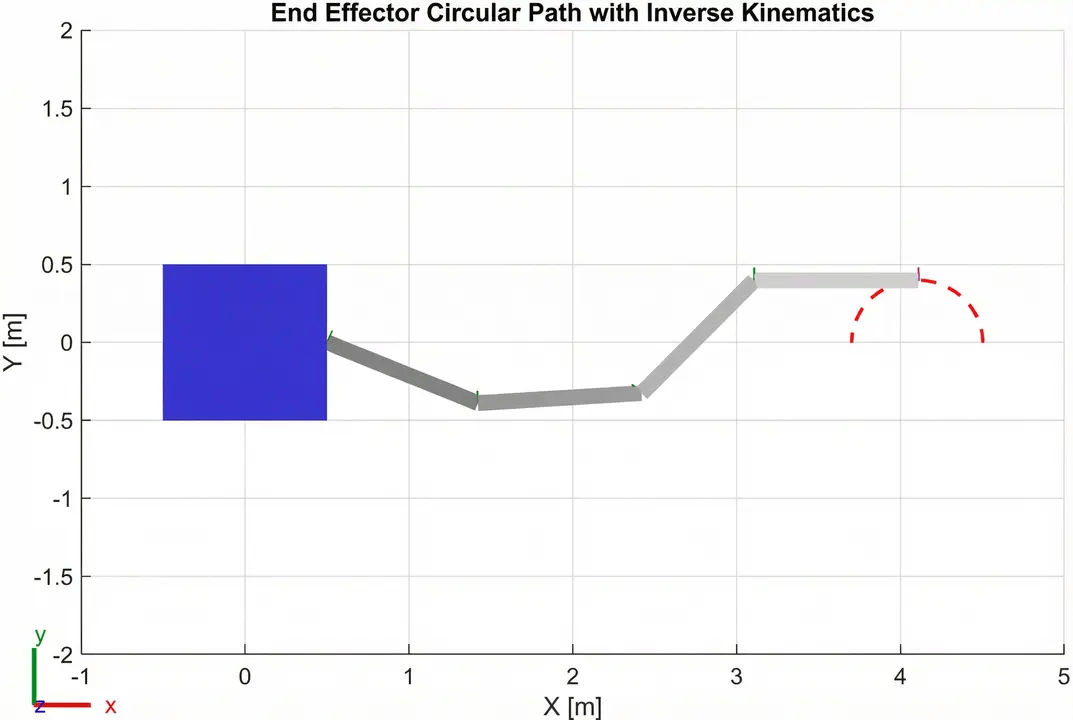
\includegraphics[width=\linewidth]{Figures/ref_kreisbahn_2.png}
    \end{subfigure}
    \vspace{0.5em}
    \begin{subfigure}{0.45\textwidth}
        \centering
        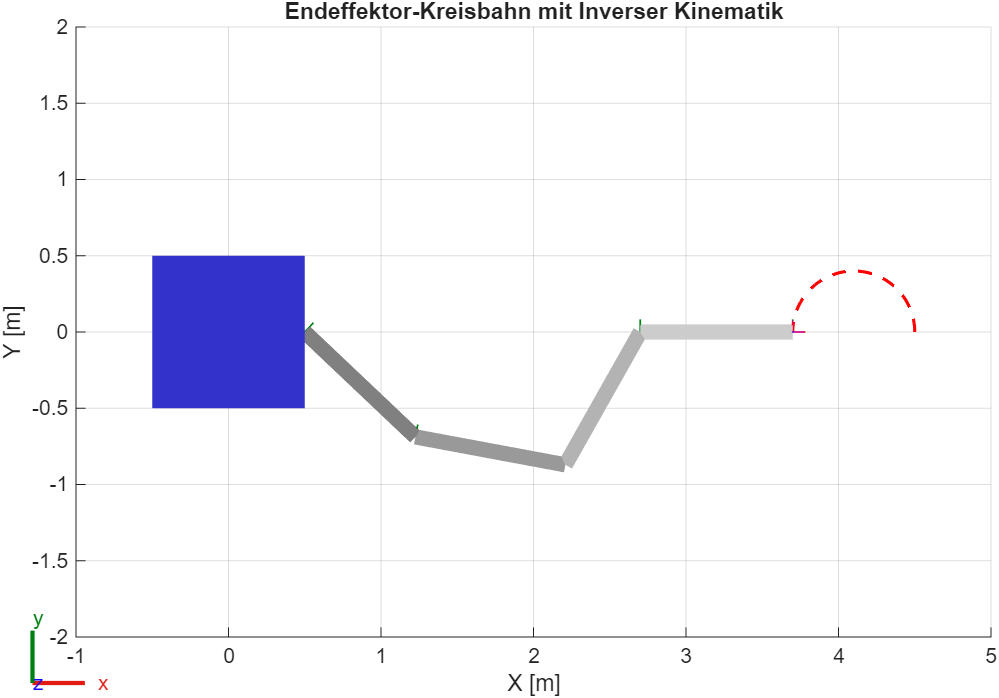
\includegraphics[width=\linewidth]{Figures/ref_kreisbahn_3.png}
    \end{subfigure}
    \caption{Tracking the desired end-effector circular path using inverse kinematics.}
    \label{fig:ref_kreis_gesamt}
\end{figure*}
\noindent
\subsection{Advantages of AI-Endowed Digital Twin Technology in On-Orbit Servicing}

AI-driven DTs have been applied in on-orbit servicing, for example for the automated lifecycle management
of satellites and for the orchestration of agents that carry out assembly, integration, and testing tasks
\cite{leutert2024ai,muhlbauer2025towards,kaigom2020value,kaigom2023metarobotics}. DTs combine
contextualized real-time sensor data with AI methods that account for uncertainty. This allows
simulation-based analysis under various operational conditions at reduced cost. Verification and
validation can also benefit, because changes in system design or operational scenarios can be described
in scenario spaces and linked to DTs \cite{maqbool2025systems}.

In this work, the DT covers only the chaser space robot. A target satellite and the contact with it are
not modeled. The DT is based on an information model that consists of the URDF description of the robot
and the parameters in \cref{tab:robot_params}. It describes the kinematics, the inertial properties, and
the joint configuration of the robot. The AI capability is provided by the deep RL agents, which are
trained and evaluated through interaction with this DT. In contrast to a classical simulation with a
pre-specified controller, the DT hosts a learning-based agent that derives its control strategy from
experience. The DT is therefore used as a training and validation environment for learned control
strategies. During training, the initial joint angles of each episode are drawn uniformly within
$\pm 1^\circ$ around the nominal configuration (see \cref{RL}). This small perturbation avoids training
from a single fixed start, but it does not cover a wide range of initial conditions.



\begin{figure*}[!t]
	\centering
	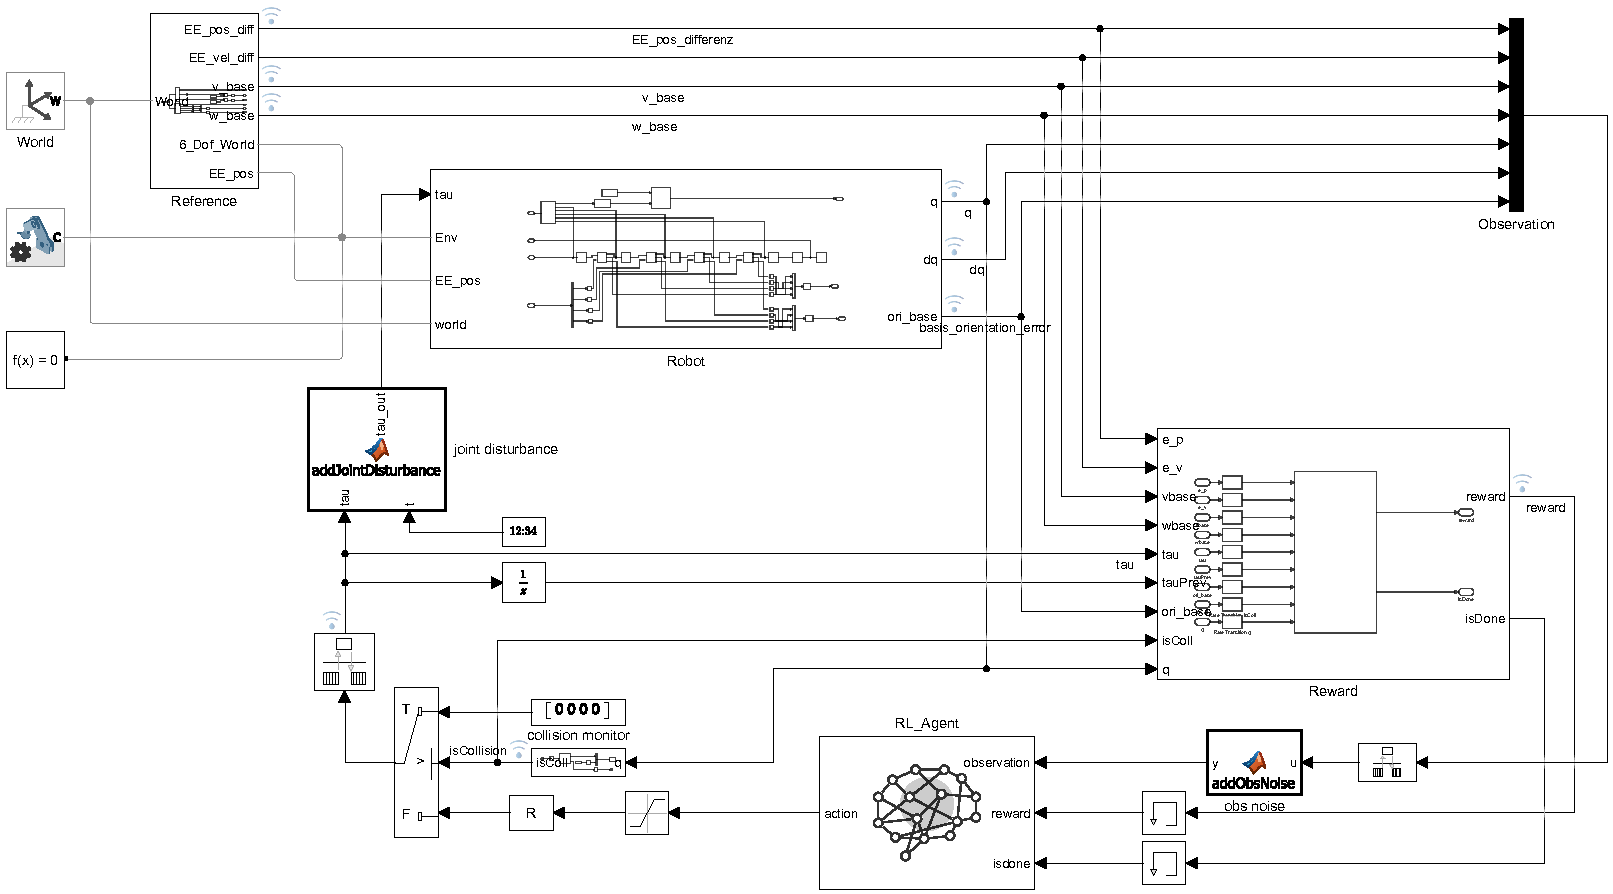
\includegraphics[width=0.98\linewidth]{Figures/Spacerobot_slx.pdf}
	\caption{Overview of the Simulink model \texttt{SpaceRobot.slx}. The closed-loop model of the free-floating space
  robot integrates the robot dynamics, reference generation, observation assembly, reward computation, and an
  RL agent block that outputs joint torques. The same model is used for all six algorithms. The reward and
  termination logic evaluate end-effector tracking, base motion, and control effort. Two further blocks add
  the observation noise and the external joint torque of the stress tests. Both are zero in the nominal
  case.}
	\label{fig:spacerobot_slx}
\end{figure*}

\subsection{Robot Model} The virtual testbed simulates a free-floating space manipulator derived from the
Spacecraft Robotics Toolkit (SPART) example \cite{b9}. The robot consists of a cuboid base (serving as
the spacecraft) and a 4-DOF serial manipulator (see~\cref{fig:ref_kreis_gesamt}). The arm has four
revolute joints and four links. Its kinematic structure and inertial properties are specified in a URDF
file (\texttt{SpaceRobot.urdf}) imported into Simulink's multibody environment \cite{b25,b26,b27}. The
geometry and the inertial parameters of the base and the links are listed in \cref{tab:robot_params}. The
same values are used in the URDF file and in the Simscape model.

\begin{table}[!t]
\centering
\caption{Parameters of the simulated free-floating space robot.}
\label{tab:robot_params}
\begin{tabular}{lc}
\toprule
\textbf{Parameter} & \textbf{Value} \\
\midrule
Base, cube with 1\,m edge length, mass & 30\,kg \\
Base, principal moments of inertia & 6\,kg\,m$^2$ \\
Links (4), length and mass & 1\,m, 2\,kg \\
Links, principal moments of inertia & 0.2\,kg\,m$^2$ \\
Viscous joint damping & 1.5\,N\,m\,s/rad \\
Joint limits $q_1$ and $q_2$ to $q_4$ & $\pm 85^\circ$ and $\pm 170^\circ$ \\
Joint-limit stiffness and damping & 3000\,N\,m/rad, 40\,N\,m\,s/rad \\
Torque limit $\tau_{\max}$ & 2\,N\,m \\
Gravity & $[0~0~0]^T$ \\
\bottomrule
\end{tabular}
\end{table}
 The resulting multibody model captures the dynamic coupling between the floating base
and the arm \cite{b6}.

\subsection{Dynamic Simulation in MATLAB/Simulink} The simulation is implemented in Simulink using the
Simscape Multibody physics engine. Gravity is set to $[0~0~0]^T$ in the mechanism configuration
\cite{b28} to emulate the microgravity orbital environment. The base is connected to the inertial world
frame through an unactuated 6-DOF joint \cite{b3}, allowing free translation and rotation. No external
forces or torques act on the system, so the base moves only in response to the internal torques
generated by the manipulator joints. Under this configuration, the total linear and angular momentum are
conserved, and arm motions induce a reactive motion of the base \cite{b6,kaigom2011optimal}.

The simulation is based on idealizing assumptions that are common in RL-based space robotics research. They are
stated here explicitly to support reproducibility and a fair comparison.
First, \emph{ideal sensing} is assumed. All state variables (joint angles, joint velocities, base orientation
quaternion, and base angular velocity) are read directly from Simulink signal buses without sensor
noise, quantization errors, or measurement bias. Second, \emph{zero communication latency} is assumed. The RL
agent receives observations and issues torque commands within the same discrete time step, with
no transmission delay between sensing and actuation. Third, the robot is modeled as a
\emph{rigid multibody system}. Flexible link dynamics, joint compliance, and thermal drift are not included.
Fourth, \emph{no external disturbances} act on the spacecraft. Gravity gradients, atmospheric drag, solar radiation
pressure, and residual magnetic torques are all set to zero, consistent with the free-floating
assumption in low-Earth orbit. These assumptions give a controlled benchmark environment. Performance differences
can therefore be attributed mainly to the algorithms rather than to environmental variability.
Consequently, the reported results characterize relative algorithm performance in a simulation benchmark under
controlled assumptions. They do not demonstrate robustness to real sensing, communication latency, structural
flexibility, or orbital disturbances, and they do not constitute an assessment of operational readiness for on-orbit
deployment. A limited stress test under non-ideal conditions is reported in \cref{sec:robustness_eval}. The
impact of the assumptions on real-world deployment is discussed in \cref{sec:discussion}.

MATLAB/Simulink was chosen as the simulation environment after considering two alternatives that are
common in robotics and RL research, Gazebo~\cite{koenig2004gazebo} and MuJoCo~\cite{todorov2012mujoco}.
MuJoCo offers an efficient contact and multibody solver and is widely used for RL benchmarks in
continuous control~\cite{korber2021comparing}. However, it has no native interface to Simulink and to
Simulink Design Verifier, which this work uses for the formal check of the torque bound. Gazebo provides
mature Robot Operating System (ROS) integration and plug-in-based sensor models and is well suited for
hardware-in-the-loop (HIL) development~\cite{collins2021review}. It offers no native path to formal
verification tools. Simscape Multibody provides a multibody solver for the free-floating
base--manipulator coupling. It runs in the same Simulink model as the runtime monitors, and Simulink
Design Verifier analyzes Simulink models without a translation step. Together with the Reinforcement
Learning Toolbox and a deterministic fixed-step solver, this gives a single reproducible toolchain from
the physical model to the learned policy and the safety checks. \cref{tab:sim_comparison} summarizes the
trade-off. This choice gives up the higher simulation speed of MuJoCo and the richer sensor and ROS
tooling of Gazebo in exchange for a close coupling of the dynamics, the RL agent, and the safety checks.

\begin{table}[!t]
\centering
\renewcommand{\arraystretch}{1.25}
\caption{Comparison of the simulation platforms considered for this work.}
\label{tab:sim_comparison}
\setlength{\tabcolsep}{4pt}
\begin{tabular}{p{2.4cm}p{1.8cm}p{1.5cm}p{1.5cm}}
\toprule
\textbf{Criterion} & \textbf{MATLAB/ Simulink} & \textbf{Gazebo} & \textbf{MuJoCo} \\
\midrule
Physics engine & Simscape Multibody & ODE, Bullet, DART & MuJoCo (native) \\
Formal verification integration & Native (Design Verifier) & None & None \\
RL framework & RL Toolbox & gym-gazebo, ROS bridges & Gymnasium, dm\_control \\
Sensor and ROS integration & Limited (via add-ons) & Extensive & Limited \\
Code generation / HIL path & Mature (Embedded Coder) & Via ROS 2 & Limited \\
Licensing & Commercial & Open source & Open source \\
\bottomrule
\end{tabular}
\end{table}

\begin{figure*}[!t]
	\centering
	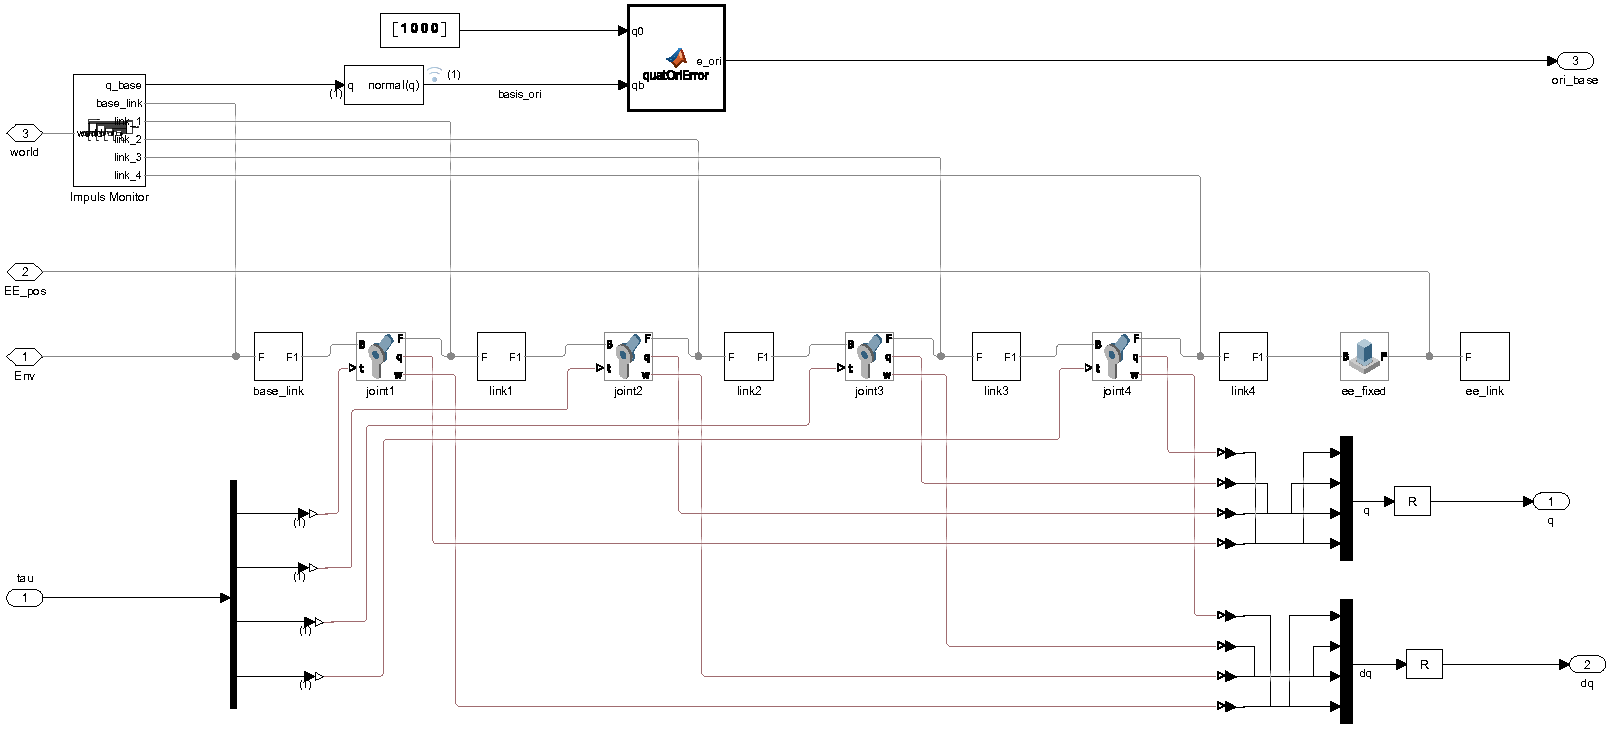
\includegraphics[width=0.98\linewidth]{Figures/spacerobot_slx_robot.pdf}
	\caption{Robot subsystem of the Simulink model \texttt{SpaceRobot.slx}. The Simscape Multibody model of the
  free-floating space robot consists of a floating base and a serial 4-DOF manipulator. Joint torque commands are
  applied to the revolute joints, and the joint positions and velocities are measured and fed back as state
  variables. The base orientation is represented as a unit quaternion and compared with a reference to compute the
  base attitude error.}
	\label{fig:spacerobot_slx_robot}
\end{figure*}

The Simulink model is composed of several subsystems, as illustrated in~\cref{fig:spacerobot_slx}. The
\emph{Robot Plant} subsystem computes the multibody dynamics of the free-floating robot at each time step
(see~\cref{fig:spacerobot_slx_robot}) by numerically integrating the equations of motion for the applied
joint torques~\cite{b6}. The \emph{Controller} subsystem executes the learned RL policy. The commanded
joint torques pass through a saturation block and a switch before reaching the plant. When the collision
monitor reports a contact, the switch overrides the torques to zero. The \emph{Reference
Trajectory Generator} provides the desired end-effector trajectory and base attitude
(see~\cref{fig:spacerobot_slx_reference}), outputting the current target position and velocity at each
time step. A set of \emph{sensors} measures the robot state (joint angles, joint velocities, base
orientation, and base angular velocity) and assembles the observation signal for the RL agent (detailed
in \cref{RL}). Finally, two \emph{safety monitors} check the operational constraints at every agent step.
The collision monitor computes the minimum distance between non-adjacent robot bodies and detects
contacts. The joint-limit monitor compares every joint angle with its admissible range. A detected
contact or a joint-limit violation terminates the episode. Details are given in \cref{formal}.

\begin{figure*}[!t]
	\centering
	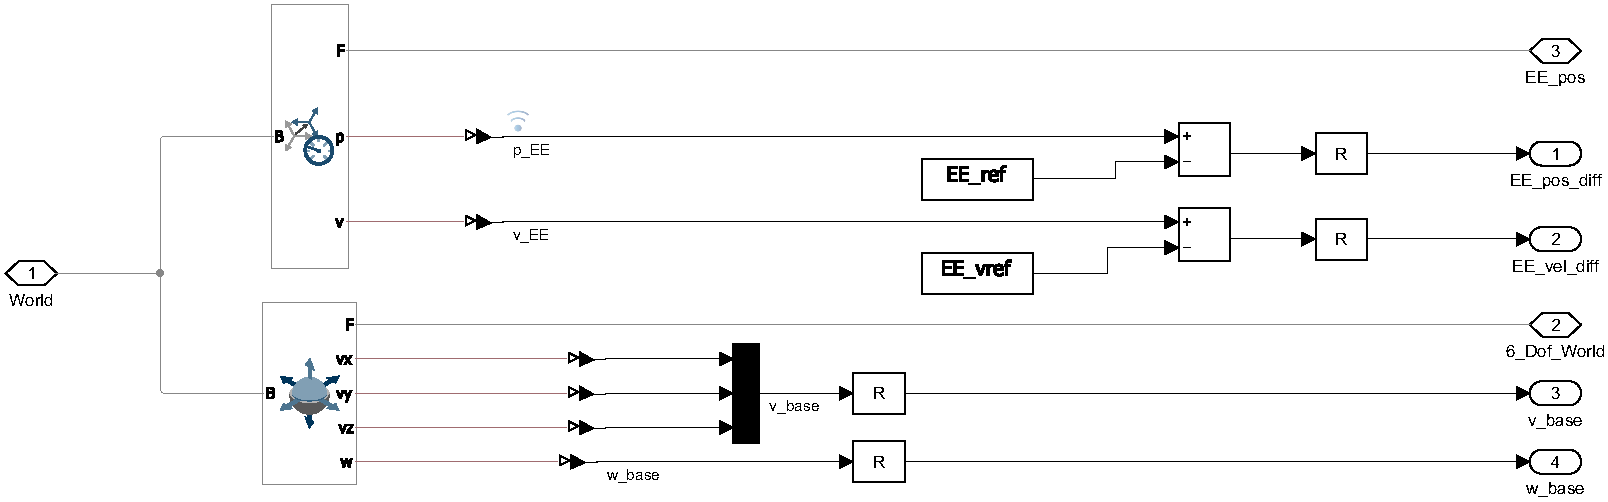
\includegraphics[width=0.97\linewidth]{Figures/spacerobot_slx_reference.pdf}
	\caption{Reference subsystem of the Simulink model \texttt{SpaceRobot.slx}. The measured end-effector position
  and velocity are compared with the reference signals. The resulting error vectors are used for the observation
  and the reward. The base linear and angular velocities are also extracted to capture the base motion induced by
  the manipulator.}
	\label{fig:spacerobot_slx_reference}
\end{figure*}

To couple the continuous dynamics with the discrete-time RL agent, a consistent integration scheme is
used. The model is simulated with a fixed-step solver (ode4) and a step size of $T_s = 0.01\,\mathrm{s}$
instead of the default variable-step solver. The agent acts every $\Delta t = 0.1\,\mathrm{s}$. Rate
transition blocks connect the two rates and hold each torque command constant over the ten solver steps
of an agent interval \cite{b29,b30}. Simulink unit consistency checks are enabled to detect modeling
errors such as mismatched units early in development.

\subsection{Reference Trajectory and Desired Task} The task is to follow a semicircular end-effector
trajectory while minimizing base disturbance. The reference starts at the end-effector position of the
stretched arm at $(4.5,\,0,\,0)\,\mathrm{m}$ and follows a semicircle with radius $r = 0.5\,\mathrm{m}$
around $(4.0,\,0,\,0)\,\mathrm{m}$ within $T = 8.5\,\mathrm{s}$ (see~\cref{fig:ref_kreis_gesamt}). The
semicircle lies in the $XY$ plane. All four joint axes are parallel to the $z$-axis, so the arm moves in
this plane and the base rotates only about the $z$-axis. The considered task is therefore planar,
although the model itself is three-dimensional. Before training, the trajectory was checked with inverse
kinematics for geometric feasibility, that is, for compliance with the joint limits and the absence of
singularities. The inverse-kinematics solution gave a consistent set of joint trajectories that realize
the desired end-effector motion. The path is therefore kinematically feasible. A failure of the RL agent
can thus be attributed to learning and not to a kinematically infeasible reference. During simulation,
the reference subsystem outputs the desired end-effector position and velocity as time series
$EE_{\mathrm{ref}}(t)$ and $EE_{v,\mathrm{ref}}(t)$ at each time step. The instantaneous position and
velocity tracking errors are derived from these signals. They enter both the observation vector and the
reward computation that penalizes large errors.

%The simulation environment provides a flexible and challenging platform for learning, with a free-floating base, a non-trivial trajectory control task, and integrated mechanisms to measure performance and enforce safety. Next, we describe how the reinforcement learning problem is formulated in this environment.

\section{Reinforcement Learning Framework}\label{RL}
\textbf{State (Observation) Space.} At each time step the RL agent receives an observation that
summarizes the state variables relevant for control \cite{b7}. The state vector consists of the
following components:
\begin{itemize}
  \item \textit{End-effector tracking error.} The Cartesian position error $e_p \in \mathbb{R}^3$ between the current
  and reference end-effector positions, together with the velocity error $e_v \in \mathbb{R}^3$. When the
end-effector is on the reference trajectory, $e_p = 0$. The pair $(e_p, e_v)$
indicates both the spatial deviation from the reference and the velocity mismatch.
  \item \textit{Arm joint states.} The joint angles $q \in \mathbb{R}^4$ and joint angular velocities
  $\dot{q} \in \mathbb{R}^4$. These describe the configuration and motion state of the manipulator. Joint
  angles are provided in radians. The joint limits are not part of the observation.
  \item \textit{Base motion.} The orientation, angular velocity, and linear velocity of the free-floating
  base. The base attitude error is computed from the measured base quaternion $q_b$ and the reference
  quaternion $q_0$ as the relative quaternion $q_{\mathrm{err}} = q_0^{*} \otimes q_b$. Its sign is
  chosen so that the scalar part is non-negative. The relative quaternion is then mapped to the
  axis--angle rotation vector $e_{\mathrm{ori}} = \theta\,\mathbf{u} \in \mathbb{R}^3$ with
  $\theta = 2\,\mathrm{atan2}(\|q_{\mathrm{err},v}\|,\,q_{\mathrm{err},w})$ and
  $\mathbf{u} = q_{\mathrm{err},v}/\|q_{\mathrm{err},v}\|$. This 3-dimensional minimal representation
  removes the redundancy of the unit-quaternion parameterization. For $q_{\mathrm{err},v} = 0$, the axis
  $\mathbf{u}$ is undefined, and $e_{\mathrm{ori}}$ is set to its limit $\theta\,\mathbf{u} \to 0$. The
  base should keep its initial attitude, so the agent has to keep $e_{\mathrm{ori}}$ close to zero. The
  base angular velocity
  $\omega_{\mathrm{base}} \in \mathbb{R}^3$ and the base linear velocity
  $v_{\mathrm{base}} \in \mathbb{R}^3$ are also included to capture the residual rotation and the
  momentum-coupled translation of the base.
\end{itemize}

The overall observation vector has dimension
$3(e_p) + 3(e_v) + 4(q) + 4(\dot{q}) + 3(\mathrm{ori}_{\mathrm{base}}) + 3(\omega_{\mathrm{base}}) + 3(v_{\mathrm{base}}) = 23$.
This state representation contains the variables required by the agent to assess tracking deviation, arm
configuration, and base motion.

\textbf{Action Space.} The action is a vector of continuous joint torque commands. At each decision step,
the agent outputs $a = [\tau_{1},\, \tau_{2}, \tau_{3},\, \tau_{4}]^T$, with one component per revolute
joint of the arm. The actions are real-valued and bounded by the actuator capabilities. Symmetric torque
limits $|\tau_{i}| \leq \tau_{\max}$ for $i = 1,\ldots,4$ are enforced through a saturation block that
clips the commanded torque to the interval $[-\tau_{\max}, +\tau_{\max}]$. The value of $\tau_{\max}$ is
selected according to the robot design ($\tau_{\max} = 2\,\mathrm{N\,m}$ in this work), provided it is
large enough to follow the reference trajectory. The saturation enforces both the actuator limits and an
upper bound on the applied torque for safety reasons. The action space is therefore the continuous box
$[-\tau_{\max}, \tau_{\max}]^4 \subset \mathbb{R}^4$, which is compatible with policy gradient and
actor-critic methods. A policy output outside this box is clipped by the saturation block.

The policy is a mapping from the 23-dimensional state space to the 4-dimensional action space,
$\pi: s \mapsto a$, parameterized by a neural network whose parameters are adjusted during training to
maximize the expected cumulative reward. The agent issues a new torque command at a fixed interval
$\Delta t = 0.1\,\mathrm{s}$. With an episode duration of $8.5\,\mathrm{s}$, this gives $N = 85$
decisions per episode.


\textbf{Reward Function Design.} The reward signal guides the agent toward accurate trajectory tracking. At the
same time, it penalizes base disturbance and favors smooth and bounded control actions.
At each discrete time step $t$, the reward $r_t$ is computed as the sum
of a progress term and a proximity bonus, minus a weighted cost function:
\begin{equation}
r_t = \frac{1}{C}\left( r_{\mathrm{prog}} + r_{\mathrm{bonus}} - c_t \right),
\label{eq:reward}
\end{equation}
where $C$ is a normalization constant.

To encourage monotonic convergence toward the reference trajectory, a progress reward is defined based
on the reduction of the end-effector position error:
\begin{equation}
r_{\mathrm{prog}} = 
\begin{cases}
k_p \left( d_{t-1} - d_t \right), & d_{t-1} > d_t,\\
0, & \text{otherwise},
\end{cases}
\end{equation}
where $d_t = \|e_p(t)\|$ is the Euclidean end-effector position error and $k_p$ is a
scaling factor. The previous distance $d_{t-1}$ is stored persistently across time steps.

A small shaping bonus is added when the end-effector is close to the reference
point:
\begin{equation}
r_{\mathrm{bonus}} = k_b \exp\!\left(-\left(\frac{d_t}{\sigma}\right)^2\right),
\end{equation}
which is intended to improve the local convergence near the desired trajectory.

The instantaneous cost $c_t$ penalizes tracking errors, base motion, and control effort:
\begin{align}
c_t =&\;
W_p \|e_p\|^2
+ W_v \|e_v\|^2
+ W_{\mathrm{ori}} \|e_{\mathrm{ori}}\|^2
+ W_{\omega_b} \|\omega_{\mathrm{base}}\|^2 \nonumber \\
&+ W_{v_b} \|v_{\mathrm{base}}\|^2
+ W_u \|\tau\|^2
+ W_d \|\tau - \tau_{t-1}\|^2 ,
\end{align}
where $e_p$ and $e_v$ denote the end-effector position and velocity errors, $e_{\mathrm{ori}}$ the base
orientation error, $v_{\mathrm{base}}$ and $\omega_{\mathrm{base}}$ the linear 
and angular base velocities, and $\tau$ the joint torque vector. The final term penalizes
changes in control input to promote smooth actuation.

The weights used in all experiments are summarized in~\cref{tab:reward_weights}. The physical intuition
behind the weight choices is as follows. The end-effector position error weight $W_p = 150$ is large
because trajectory tracking is the primary task objective. A high weight makes the position error the
dominant term of the cost at typical error magnitudes. The velocity error weight $W_v = 25$ is lower than
$W_p$ to avoid over-penalizing transient dynamics during fast arm motion, while still discouraging
persistent velocity offsets. The base orientation weight $W_{\mathrm{ori}} = 200$ is the largest weight
in the cost function, because base attitude disturbance is safety-critical in on-orbit operations. An
uncontrolled rotation of the spacecraft base can endanger the mission regardless of the tracking
performance. The base angular velocity weight $W_{\omega_b} = 8$ penalizes ongoing base rotation, similar
to a damping term. The linear velocity weight $W_{v_b} = 2$ is kept small. With zero initial linear
momentum, base translation is coupled to the manipulator motion and is expected to remain small for the
considered task. It cannot be avoided completely, because the center of mass of the whole system stays
fixed. The torque magnitude weight $W_u = 0.02$ and the torque-rate weight $W_d = 0.06$ are small so that
the agent keeps enough freedom to explore different control actions. The torque-rate penalty is slightly
larger to discourage high-frequency chattering in the control signal. The progress scaling factor
$k_p = 10$ is chosen so that the progress reward has a magnitude comparable to the cost terms at
typical error levels and is not dominated by them. The proximity bonus parameters $k_b = 0.05$ and
$\sigma = 0.02$ are small by design. They provide a weak local guidance signal near the trajectory
without creating a strong local attractor that could trap the policy. Finally, the normalization constant
$C = 500$ scales the total reward to a range of approximately $[-1,\, 0]$ under typical operating
conditions, which is intended to stabilize the value-function learning of all tested algorithms.

At each step, all inputs to the reward function are checked for numerical validity. An episode is
terminated early if a NaN or Inf value is detected, if the end-effector error exceeds $10\,\mathrm{m}$,
if the collision monitor reports a contact, or if a joint leaves its admissible range. In that case,
the agent receives the lower end of the one-step reward range, $-1$, for the terminal step and for
every remaining step of the episode. The terminal penalty is therefore
\begin{equation}
r_{\mathrm{fail}} = -\,(N - k + 1),
\label{eq:rfail}
\end{equation}
where $k$ is the step at which the violation occurs and $N = 85$ is the number of steps
per episode. A constant penalty is not sufficient in this setting. The step rewards are negative in
nearly all states, so a single penalty of $-1$ would make an early termination more attractive than
continuing with a poor policy. In a pilot run with a constant penalty of $-1$, none of the
last 100 training episodes of the default and the optimized PPO agent reached the end of the horizon.
With the penalty in \eqref{eq:rfail}, all of them did. All reward components were implemented in a MATLAB
Function block within the Simulink environment.

\begin{table}[!b]
\centering
\caption{Reward function weights used in all experiments.}
\label{tab:reward_weights}
\begin{tabular}{lcc}
\toprule
\textbf{Term} & \textbf{Symbol} & \textbf{Value} \\
\midrule
End-effector position error      & $W_p$              & 150   \\
End-effector velocity error      & $W_v$              & 25    \\
Base orientation error           & $W_{\mathrm{ori}}$   & 200   \\
Base angular velocity            & $W_{\omega_b}$     & 8     \\
Base linear velocity             & $W_{v_b}$          & 2     \\
Joint torque magnitude           & $W_u$              & 0.02  \\
Torque rate (smoothness)         & $W_d$              & 0.06  \\
Progress scaling factor          & $k_p$              & 10    \\
Proximity bonus scaling          & $k_b$              & 0.05  \\
Proximity width                  & $\sigma$           & 0.02  \\
Reward normalization constant    & $C$                & 500   \\
\bottomrule
\end{tabular}
\end{table}

\textbf{Training Procedure.} An episodic training scheme is used. Each episode covers the semicircular
reference once and lasts $T = 8.5\,\mathrm{s}$, which corresponds to $N = 85$ agent steps. At the start
of each episode, a custom reset function sets the base to its home orientation at rest. The initial
joint angles are drawn uniformly within $\pm 1^\circ$ around the nominal stretched configuration $q = 0$,
in which the end-effector is located at the start of the reference. These initial states lie close to
a configuration that is free of collisions and far from the joint limits. All state variables, integrator
states, and logging signals are reset as well.

Within an episode, the agent receives an observation at each step and outputs a torque action. The
simulation runs until the end of the horizon or until one of the terminal conditions of the reward
function occurs. In that case the penalty in \eqref{eq:rfail} is applied and the episode ends at that
step.

The training loop is provided by MATLAB's Reinforcement Learning Toolbox. After each episode or after a
fixed number of steps, the collected states, actions, and rewards are used to update the policy according
to the chosen RL algorithm \cite{b4}. Where applicable, the value function is updated as well. The
algorithm-specific update rules of PPO, DDPG, and the remaining methods are handled by their respective
toolbox implementations. This work supplies the experience and the reward signal. All agents
are trained for the same number of episodes, $N_{\mathrm{train}} = 1000$. This budget is intended to let
most algorithms converge or reach a performance plateau. During training, the cumulative reward and the
length of every episode are recorded. A successful training run is characterized by an episode return
that increases toward zero, since the step rewards are negative costs. An episode that ends before $N$
steps was terminated by a monitor, so the episode length also shows how often safety violations occur
during training.

To make the runs reproducible, MATLAB's Mersenne Twister random number generator is initialized with a
seed $s$ before each training run (\texttt{rng(s,\textquotesingle twister\textquotesingle)}). The seed
determines the initial network weights, the exploration noise, the sampling of mini-batches, and the
initial joint angles of every episode. Two runs with the same seed are identical. Each configuration was
trained with ten seeds ($s = 0,\dots,9$). This results in 70 training runs for the six default agents
and the optimized PPO agent. Ten seeds are used so that the seed-level tests keep some resolution
after the correction for multiple comparisons. Every run comprises exactly
$N_{\mathrm{train}} = 1000$ episodes without early stopping, and the policy after the last episode is
evaluated. No checkpoint is selected, and all ten seeds are reported.

\textbf{Evaluation and Metrics.} After training, each policy is evaluated deterministically. For the
stochastic policies, the mean action is used. Every policy is evaluated on $N_{\mathrm{eval}} = 30$
episodes whose initial joint angles are drawn uniformly within $\pm 1^\circ$ from a fixed random stream,
and on one additional episode from the nominal start pose. All agents use the same initial states, so
the evaluation episodes are paired across agents. The conclusions therefore remain conditional on these
initial states and the tested reference trajectories. Over the evaluation episodes, a set of Key
Performance Indicators (KPIs) is computed to compare the agents quantitatively. For episodes that
terminate early due to a safety violation, each KPI is computed over the executed portion of the episode
up to the termination step.

The KPIs are first computed for each seed over the 30 random episodes. The seed dependence and the
performance reached are then reported separately. A training run counts as successful when none of its
31 evaluation episodes is terminated by a monitor. The first table reports the number of successful runs
per configuration and the share of evaluation episodes that a monitor terminated, taken over all runs.
The KPI tables report the mean and the standard deviation over the successful runs only, together with
their number. These KPI values are therefore conditional on a successful run.

Algorithms are compared on the seed level with two-sided Mann--Whitney $U$ tests over the successful
runs. A test is reported only when both configurations have at least four successful runs. The shares of
successful runs are compared with Fisher's exact test. In both cases, the $p$-values are Holm-corrected
over the agents that are compared with the same reference. For the KPIs, this correction is applied
separately to each KPI and does not cover the number of KPIs. When a single agent is compared with TRPO,
the reported $p$-values are therefore uncorrected. In these cases, the text also states the result of a
Holm correction over the seven tested KPIs. The KPIs $K_5$ and $K_6$ are zero in every successful run and
are not tested.

The nine KPIs are organized into three groups to aid interpretation. The \emph{tracking accuracy}
group ($K_2$ and $K_3$) measures how closely the end-effector follows the reference path. The
\emph{base stability and safety} group covers spacecraft attitude drift ($K_4$) and constraint violations ($K_5$
and $K_6$). The \emph{efficiency} group covers control smoothness ($K_7$), residual base rotation ($K_8$), and
energy consumption ($K_9$). $K_1$ is an overall scalar summary of the agent's performance
across all objectives, since it is the cumulative reward that jointly penalizes all undesired
behaviors.

\begin{itemize}
  \item $\boldsymbol{K_1}$ (\emph{Mean Episodic Return}). Mean cumulative reward per episode. Higher is better and
  reflects overall task success.
  \begin{equation*}
  R_i=\sum_{k=1}^{T_i} r_i[k], \qquad K_1=\frac{1}{N_{\mathrm{eval}}}\sum_{i=1}^{N_{\mathrm{eval}}} R_i.
  \end{equation*}

  \item $\boldsymbol{K_2}$ (\emph{Mean Squared EE Position Error}). Average squared tracking error per episode. Lower
  is better.
  \begin{equation*}
  K_2=\frac{1}{N_{\mathrm{eval}}}\sum_{i=1}^{N_{\mathrm{eval}}}\frac{1}{T_i}\sum_{k=1}^{T_i}\|e_{p,i}[k]\|_2^2.
  \end{equation*}

  \item $\boldsymbol{K_3}$ (\emph{Maximum EE Position Error}). Worst-case tracking deviation. Lower is better.
  \begin{equation*}
  K_3=\max_{i}\max_{k}\|e_{p,i}[k]\|_2.
  \end{equation*}

  \item $\boldsymbol{K_4}$ (\emph{Mean Base Orientation Error}). Average attitude drift of the spacecraft base, measured
  as the magnitude of the axis--angle rotation-vector error $e_{\mathrm{ori}}$ (in radians). Lower is better.
  \begin{equation*}
  K_4=\frac{1}{N_{\mathrm{eval}}}\sum_{i=1}^{N_{\mathrm{eval}}}\frac{1}{T_i}\sum_{k=1}^{T_i}\|e_{\mathrm{ori},i}[k]\|_2.
  \end{equation*}

  \item $\boldsymbol{K_5}$ (\emph{Collision Rate}). Fraction of episodes with at least one collision. Zero is
  ideal.
  \begin{equation*}
  C_i=\mathbb{I}(\exists k:\,c_i[k]>0.5), \qquad K_5=\frac{1}{N_{\mathrm{eval}}}\sum_{i=1}^{N_{\mathrm{eval}}} C_i.
  \end{equation*}

  \item $\boldsymbol{K_6}$ (\emph{Joint Limit Violation Rate}). Fraction of joint samples outside the
  mechanical limits, averaged over all joints and time steps of an episode. Zero is ideal.
  \begin{equation*}
  \begin{aligned}
  K_6 &= \frac{1}{N_{\mathrm{eval}}}\sum_{i=1}^{N_{\mathrm{eval}}}\frac{1}{T_i n_J}\sum_{k=1}^{T_i}\sum_{j=1}^{n_J}
  V_{i,j}[k],\\
  V_{i,j}[k] &= \mathbb{I}\!\big(q_{i,j}[k]\notin[q_j^{\min},q_j^{\max}]\big).
  \end{aligned}
  \end{equation*}

  \item $\boldsymbol{K_7}$ (\emph{Control Smoothness (Jerk)}). Second difference of joint torques. Lower
  values indicate smoother, less chattering actuation.
  \begin{equation*}
  \begin{aligned}
  \Delta^2\tau_i[k] &= \tau_i[k+2]-2\tau_i[k+1]+\tau_i[k],\\
  J_i &= \frac{1}{T_i-2}\sum_{k=1}^{T_i-2}\|\Delta^2\tau_i[k]\|_2,\\
  K_7 &= \frac{1}{N_{\mathrm{eval}}}\sum_{i=1}^{N_{\mathrm{eval}}}J_i.
  \end{aligned}
  \end{equation*}

  \item $\boldsymbol{K_8}$ (\emph{Mean Base Angular Velocity}). Residual spacecraft rotation rate during
  the task (rad/s). Lower is better, ideally zero.
  \begin{equation*}
  K_8=\frac{1}{N_{\mathrm{eval}}}\sum_{i=1}^{N_{\mathrm{eval}}}\frac{1}{T_i}\sum_{k=1}^{T_i}\|\omega_{b,i}[k]\|_2.
  \end{equation*}

  \item $\boldsymbol{K_9}$ (\emph{Energy Consumption}). Average absolute mechanical power integrated over
  each episode. Lower is better when not at the expense of tracking quality.
  \begin{equation*}
  \begin{aligned}
  E_i &= \int\sum_{j=1}^{n_J}\big|\tau_{i,j}(t)\,\dot q_{i,j}(t)\big|\,dt,\\
  K_9 &= \frac{1}{N_{\mathrm{eval}}}\sum_{i=1}^{N_{\mathrm{eval}}} E_i.
  \end{aligned}
  \end{equation*}
\end{itemize}


Two KPIs need a justification in the context of space missions. The control smoothness $K_7$ captures
high-frequency torque oscillations (chattering). In space, such oscillations can accelerate actuator wear
and excite structural vibrations. These vibrations degrade the pointing accuracy of sensitive instruments
such as cameras or star trackers. Rapid back-and-forth motion also dissipates energy. Minimizing $K_7$
therefore supports hardware lifetime and payload pointing requirements. The energy consumption $K_9$
reflects the mechanical work performed by the joints, approximated as
$\int \sum_j |\tau_j \dot{q}_j|\,dt$. Onboard power is limited by solar panel area and battery capacity.
Energy spent on control actuation reduces the budget available for communication, thermal management, and
payload operation. Reducing $K_9$ without sacrificing tracking accuracy therefore has operational value
for mission planning.

In addition to the KPIs above, two training-related metrics are reported. $T_1$ is the standard deviation
of the episode reward over the last 100 training episodes, an indicator of training stability. $T_2$ is
the wall-clock training time required for 1000 episodes, an indicator of the computational load.

Applying these metrics to all six agents yields a common basis for comparison. The
comparative results are presented and discussed in \cref{comparison}.

\section{Safety Monitoring and Constraint Enforcement}\label{formal}
Stability and safety are central requirements in space robotics. A controller for autonomous on-orbit
servicing must satisfy the physical constraints of the system and avoid hazardous states, in
particular when the control policy is learned from data and must therefore handle uncertainty.
In this work, runtime safety monitors and constraint-enforcement mechanisms are integrated directly into the
RL training and execution environment. They have two purposes. They terminate episodes that reach unsafe states
during exploration, and they shape the agent's behavior toward the monitored constraints through
penalties~\cite{b7,b22}. These mechanisms address a defined set of properties and do not constitute a
formal safety certification of the learned controller (see the limitations at the end of this section).

\begin{figure*}[!t]
\centering
   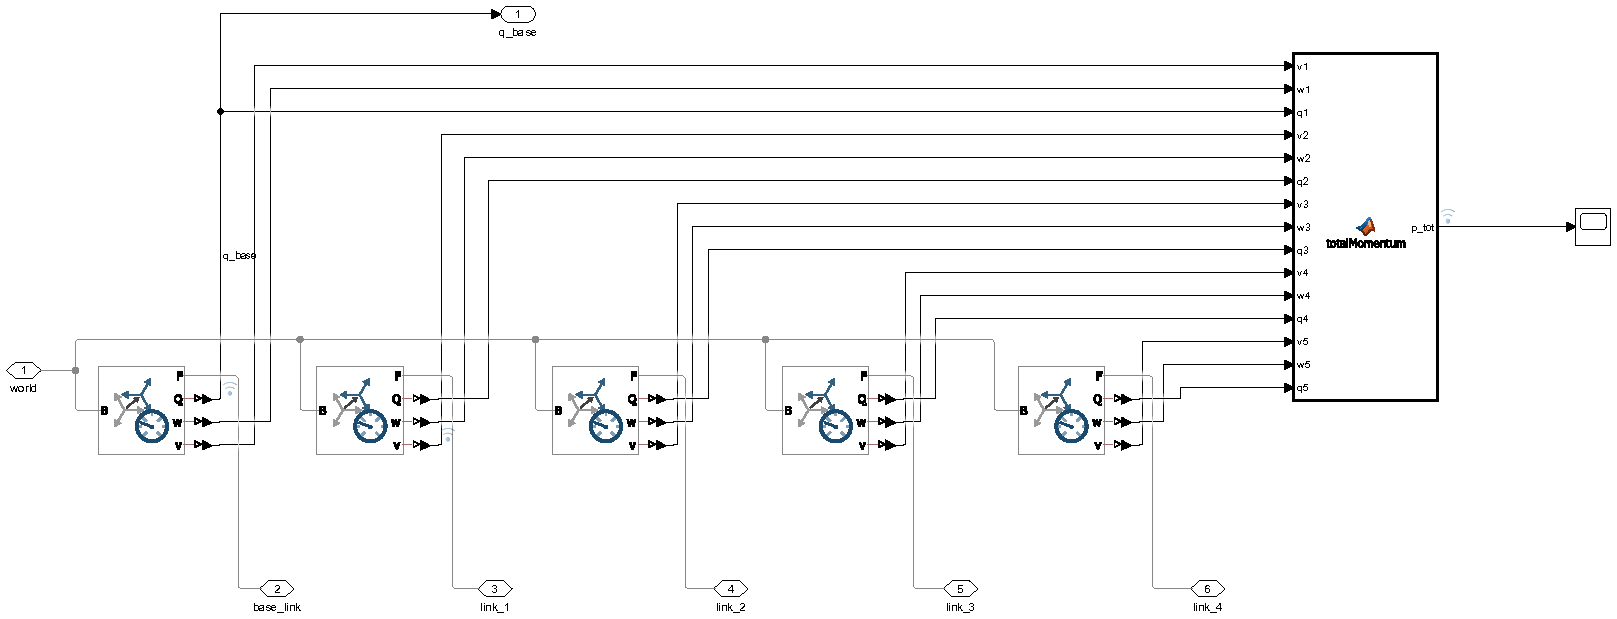
\includegraphics[width=1\linewidth]{Figures/impuls_monitor.pdf}
    \caption{Momentum monitor subsystem (momentum observer) of the Simulink model \texttt{SpaceRobot.slx}. The
    velocities and orientations of the base and of all manipulator links are measured and combined in a MATLAB
    function to compute the total linear momentum of the free-floating space robot. The monitor is used to check
    momentum conservation in the simulation.}
    \label{fig:impuls_monitor}
\end{figure*}
\begin{figure}[!b]
  \centering
  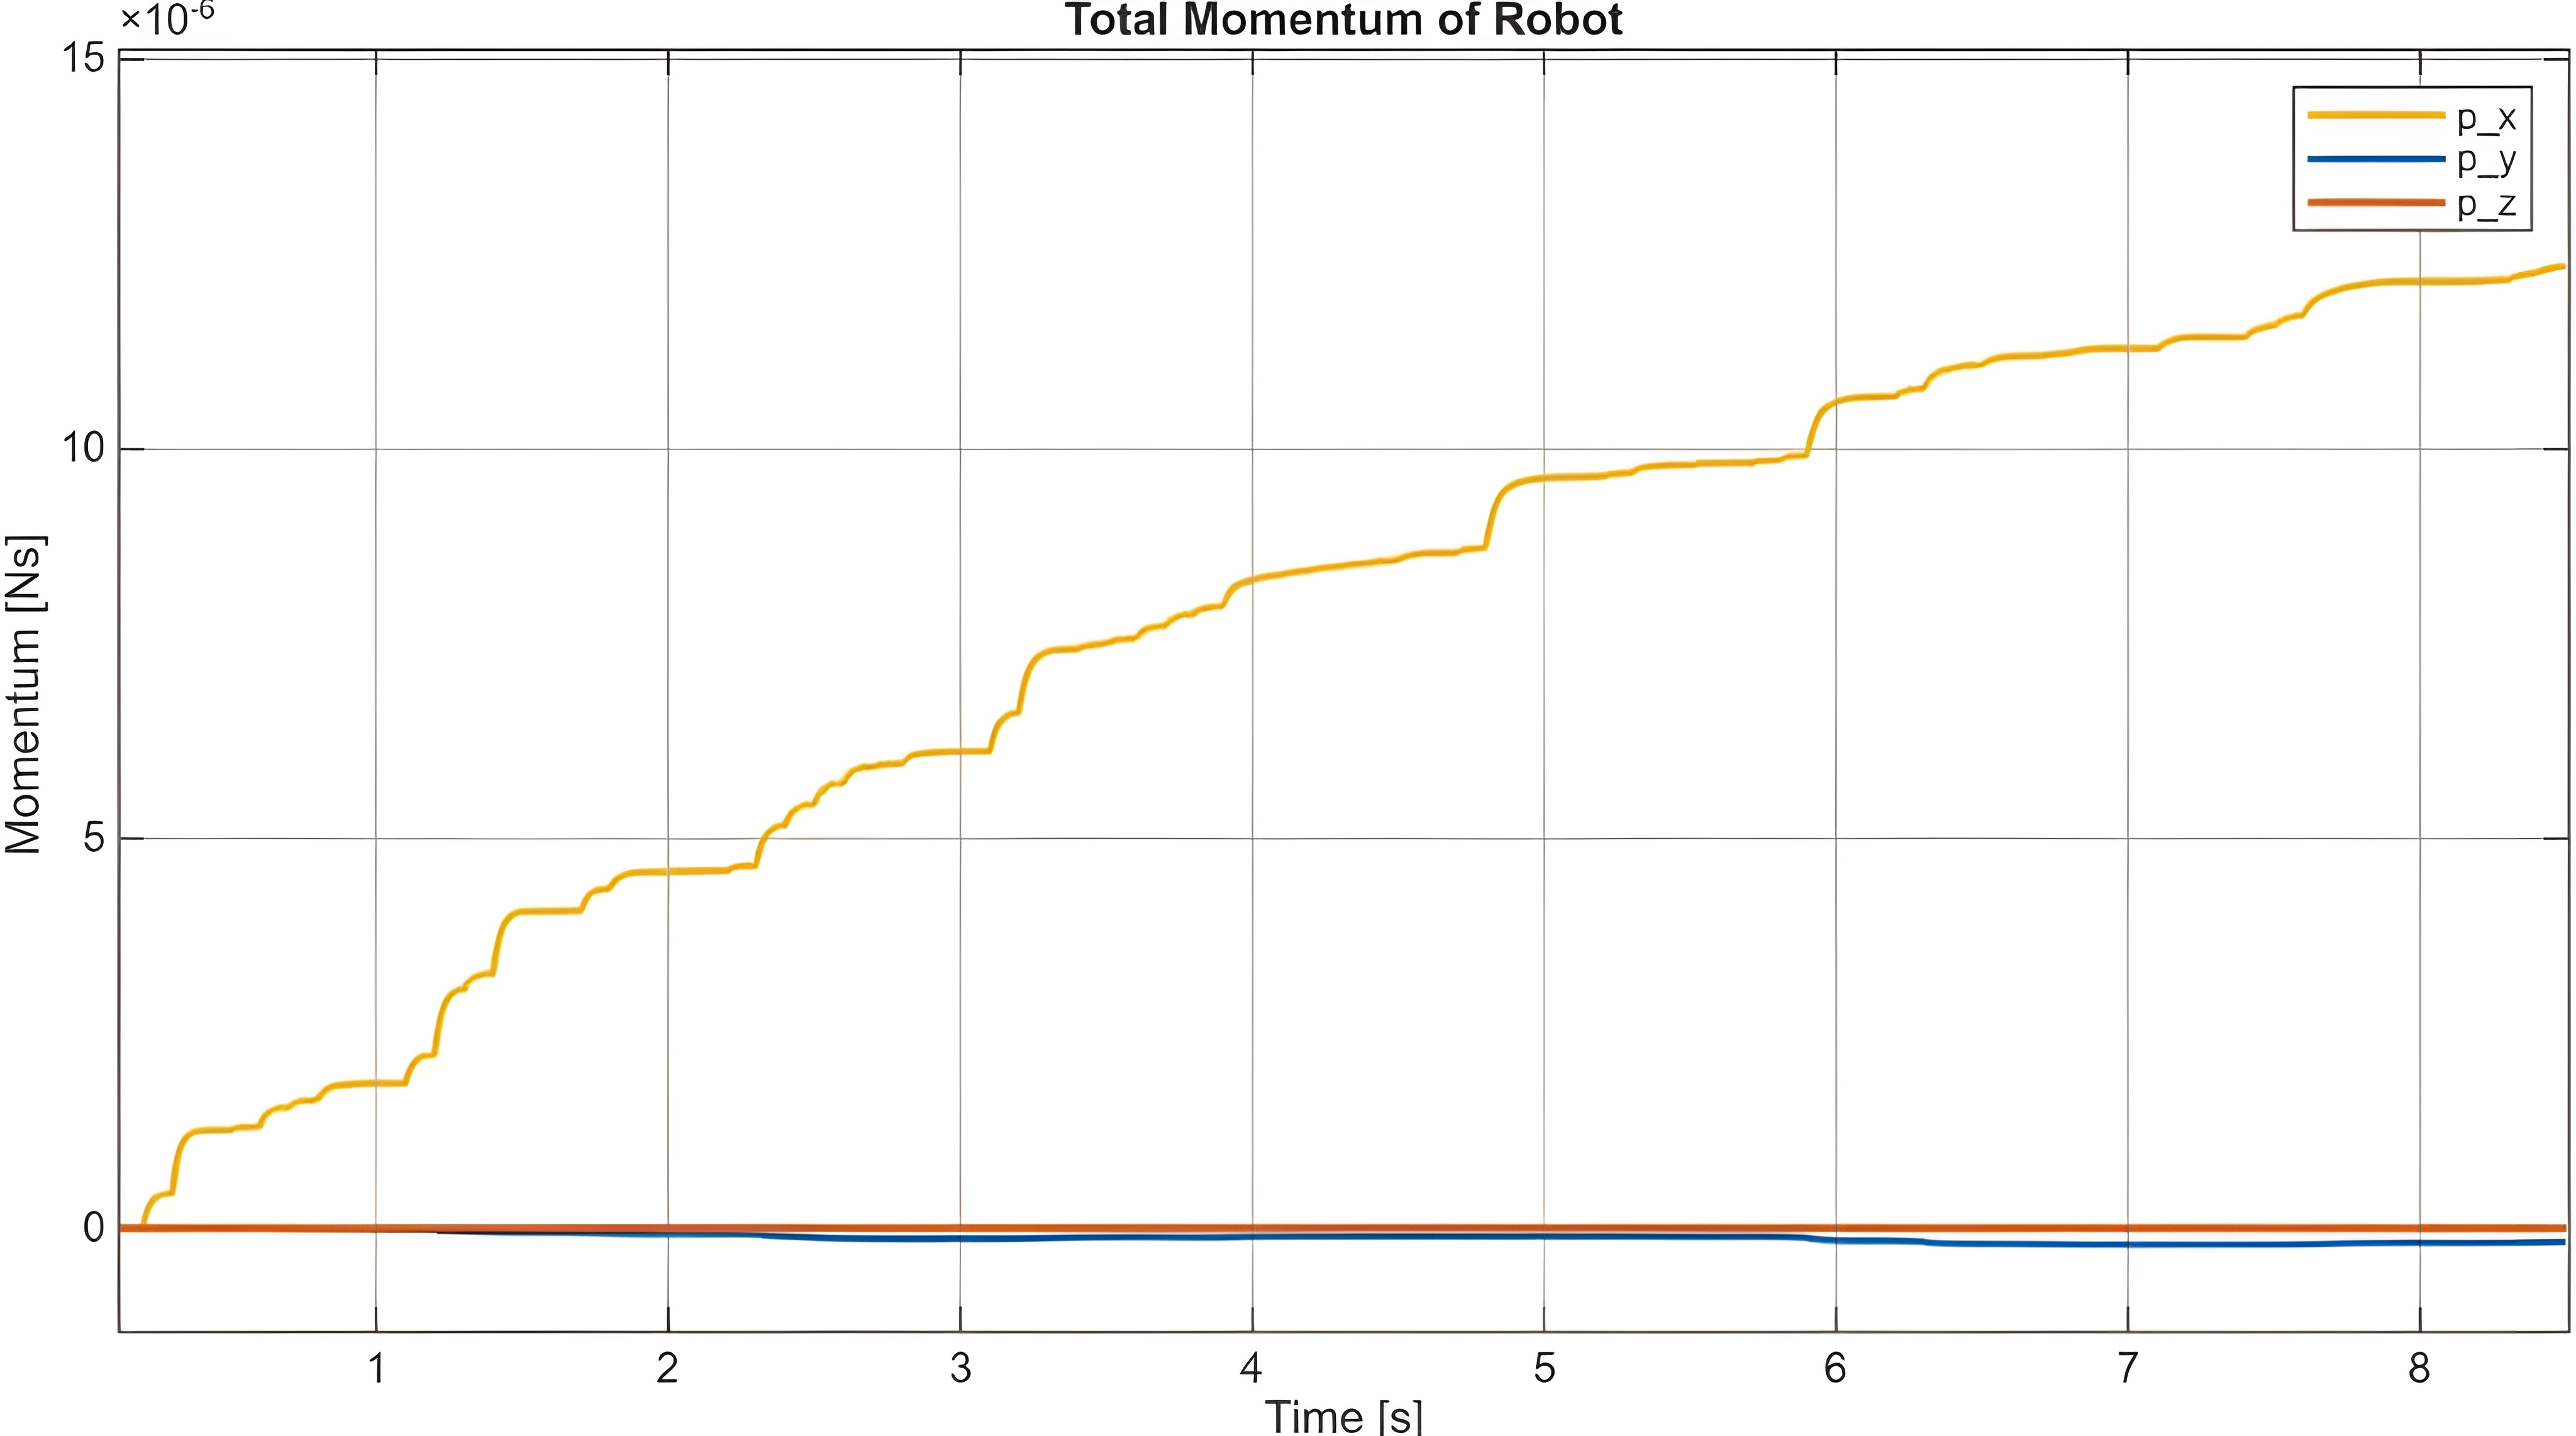
\includegraphics[width=0.95\linewidth]{Figures/impulserhaltung_scope.png}
  \caption{Total linear momentum of the robot during an episode.}
  \label{fig:impulserhaltung_scope}
\end{figure}
\textbf{Momentum Conservation Monitor.} In a free-floating system without external forces, both the total
linear and the total angular momentum of the robot (base and arm) are conserved. With zero initial
momentum, the total linear momentum remains close to zero throughout the simulation \cite{b6}. A momentum
observer computes the total linear momentum $p_{\mathrm{tot}}$ and checks for its conservation (see
\cref{fig:impuls_monitor}). Virtual sensors attached to the base and to each link provide the body
velocities, from which $p_{\mathrm{tot}} = \sum_{i} m_{i} v_{i}$ is computed. In an ideal
simulation, $p_{\mathrm{tot}}$ remains close to zero throughout an episode. Small numerical
deviations may arise from time-integration errors. A persistent, systematic drift of $p_{\mathrm{tot}}$
would indicate an unintended external force or a modeling error, such as an unmodeled constraint.
\cref{fig:impulserhaltung_scope} shows $p_{\mathrm{tot}}$ for an evaluation episode of the
optimized PPO agent from the nominal initial state. An offset of $2.7 \times 10^{-7}\,\mathrm{N\,s}$
appears in the first agent step, after which $p_{\mathrm{tot}}$ stays constant. For TRPO and the
optimized PPO agent, $|p_{\mathrm{tot}}|$ remained below $10^{-6}\,\mathrm{N\,s}$ in all 620 evaluation
episodes. The other agents reached up to $4.3 \times 10^{-4}\,\mathrm{N\,s}$. These larger deviations
may be explained by the integration error of the fixed-step solver for rapidly changing torque commands.
The values indicate that the simulation conserves momentum within the numerical tolerance. The
momentum observer is a diagnostic tool. It is evaluated offline and does not influence the training.

\begin{figure*}[!t]
    \centering    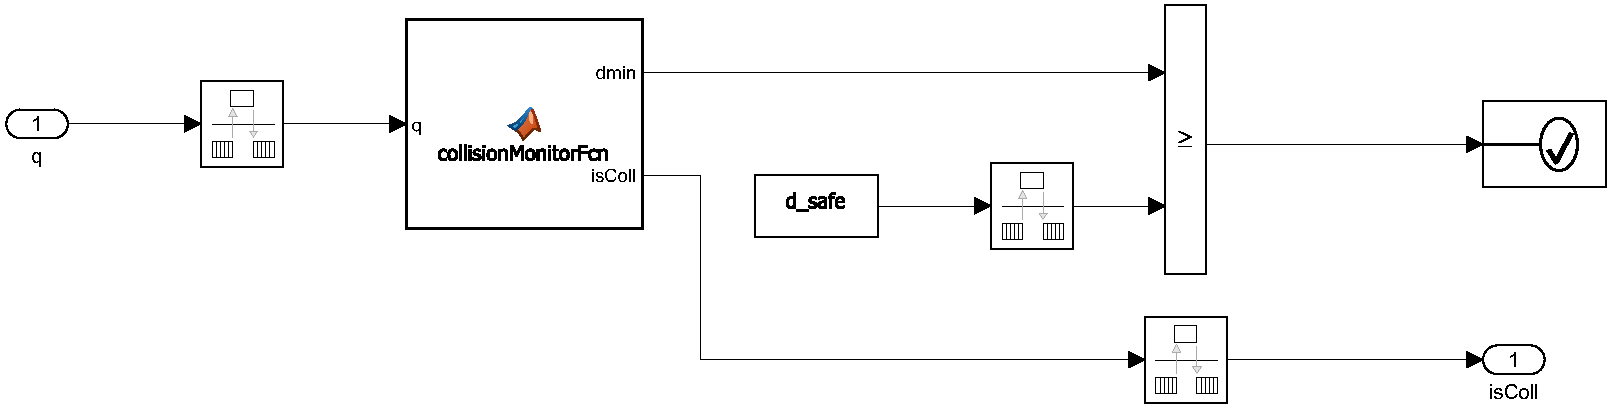
\includegraphics[width=0.75\linewidth]{Figures/spacerobot_slx_colissionmonitor.pdf}
    \caption{Collision monitor subsystem of the Simulink model \texttt{SpaceRobot.slx}. The joint angles $q$
    are used to compute the minimum distance between non-adjacent robot bodies. A distance below the safety
    threshold $d_{\mathrm{safe}}$ triggers the assertion block, which raises a warning. A detected contact sets
    the collision flag, which terminates the episode.}
    \label{fig:spacerobot_slx_colissionmonitor}
\end{figure*}

\begin{figure*}[!t]
    \centering
    \begin{subfigure}[b]{0.48\textwidth}
        \centering
        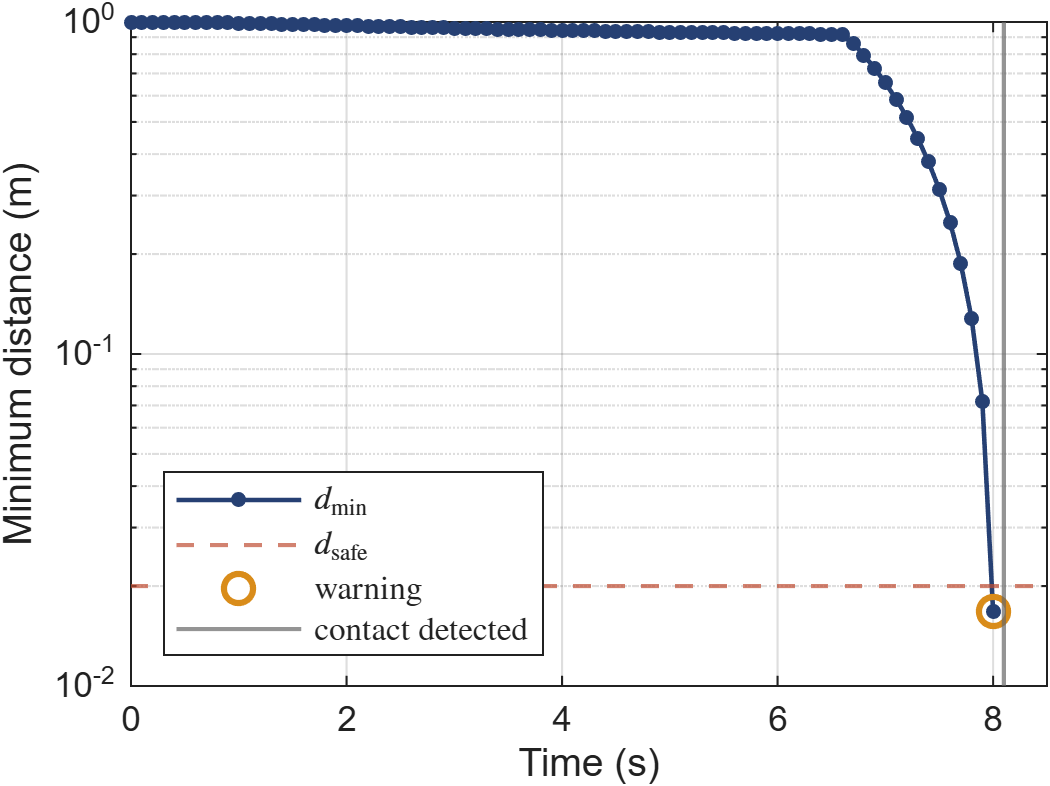
\includegraphics[width=\linewidth]{Figures/collision_test_dmin.png}
        \caption{Minimum distance between non-adjacent bodies}
        \label{fig:collision_dmin}
    \end{subfigure}
    \hfill
    \begin{subfigure}[b]{0.48\textwidth}
        \centering
        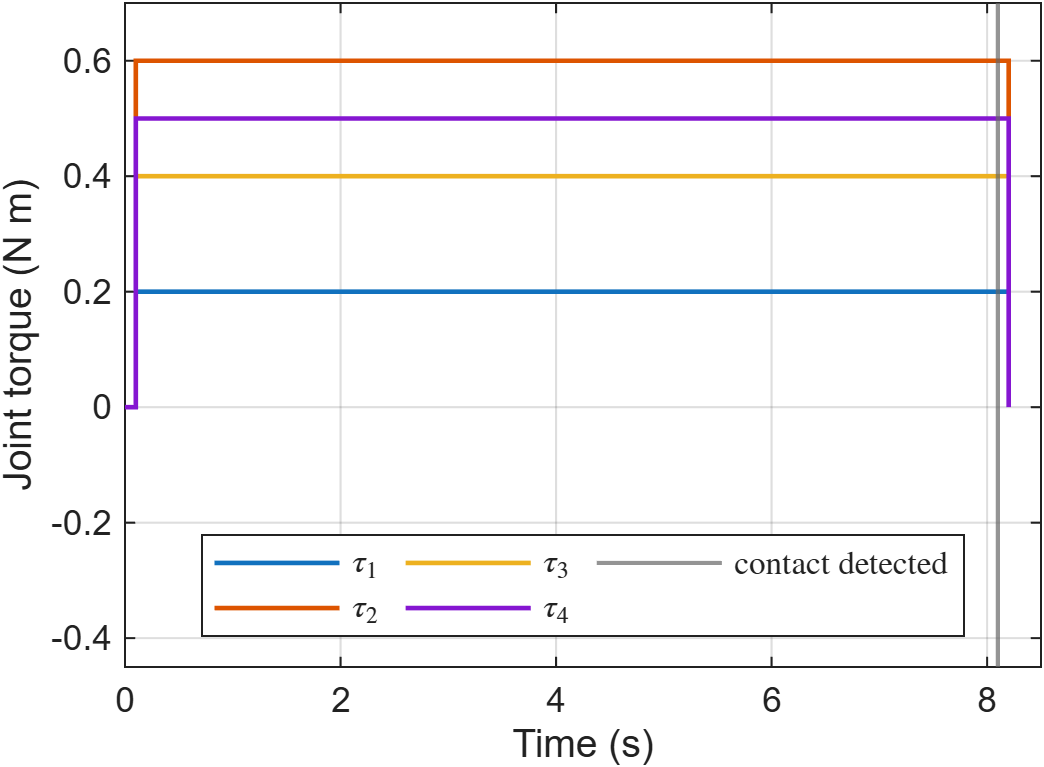
\includegraphics[width=\linewidth]{Figures/collision_test_tau.png}
        \caption{Commanded joint torques}
        \label{fig:collision_tau}
    \end{subfigure}
    \caption{Test of the collision monitor with constant joint torques that fold the arm toward the base. The
    warning is raised when $d_{\min}$ falls below $d_{\mathrm{safe}}$. After the detected contact, the torques
    are set to zero and the episode ends at $t = 8.2\,\mathrm{s}$.}
    \label{fig:collision_combined}
\end{figure*}
\textbf{Collision Monitor.} At every agent step, a collision monitor computes the minimum distance
$d_{\min}$ between non-adjacent robot bodies (see \cref{fig:spacerobot_slx_colissionmonitor}). The
monitor is a MATLAB Function block that applies the \texttt{checkCollision} function of the Robotics
System Toolbox \cite{b31} to the collision geometry of the URDF model. If $d_{\min}$ falls below the
safety threshold $d_{\mathrm{safe}} = 2\,\mathrm{cm}$, a warning is raised and logged. If a contact
between two bodies is detected, all commanded joint torques are overridden to zero and the episode is
terminated with the penalty in \eqref{eq:rfail}.

The monitor was tested in two cases without a trained agent. In the first case, constant joint torques
of 0.2, 0.6, 0.4, and 0.5\,N\,m folded the arm from the nominal pose toward the base
(\cref{fig:collision_combined}). The distance $d_{\min}$ fell below $d_{\mathrm{safe}}$ at
$t = 8.0\,\mathrm{s}$, and the warning was raised. The contact was detected at $t = 8.1\,\mathrm{s}$.
At the next agent step, the torques were set to zero and the episode ended. In the second case, an
episode started in a colliding configuration and was terminated after the first agent step. With larger
torques, $d_{\min}$ can drop from above $d_{\mathrm{safe}}$ to a contact within one agent step. The
warning therefore does not always precede the contact. During training, collisions occurred mainly in
early exploratory episodes. The monitor detected them and terminated the episode. In the evaluation of
the 70 trained agents, 108 of 2170 episodes ended with a detected contact. These episodes belong to six
runs of DDPG, TD3, PG, and the default PPO agent. No contact occurred in the evaluation episodes of TRPO,
SAC, and the optimized PPO agent.

\textbf{Joint Limit Enforcement.} Each revolute joint of the arm is subject to mechanical limits.
Violating these limits could damage a real robot and often indicates an unstable controller. The joint
limits are enforced at two levels. First, the Simscape model includes mechanical joint limits with
penalty forces, i.e., a stiff barrier that opposes further motion beyond the limit. Second,
a joint-limit monitor in the reward block compares every joint angle with its admissible range at each
agent step. A violation terminates the episode with the penalty in \eqref{eq:rfail}, which
prevents further motion into the limit. In the evaluation of the 70 trained agents,
joint-limit violations terminated 791 of the 2170 episodes. They were the most frequent reason for a
terminated episode. TRPO and the optimized PPO agent reached no joint limit in any evaluation episode.
Because a violation ends the episode, the joint limit violation rate $K_6$ is zero for every run without
a terminated episode. The violations are therefore reported as abort rates in \cref{tab:robustness_seeds}.

\textbf{Formal Check of the Torque Bound.} In addition to the runtime monitors, the torque bound of the
actuation path was checked formally with Simulink Design Verifier (SLDV) in property-proving mode
\cite{b5}. \cref{fig:verify_tau} shows the verification model \texttt{verify\_tau.slx}. It contains a
saturation block with the same limits $\pm\tau_{\max}$ as the actuation path of \texttt{SpaceRobot.slx}.
The commanded torque vector $\tau$ enters this block as an unconstrained input. A proof objective requires
$|\tau_i| \leq \tau_{\max}$ for each saturated component. SLDV proved this objective valid and found no
counterexample (\cref{fig:verify_tau_result}). Because the input is unconstrained, the bound holds for any
output of the trained policy, including outputs in states that were not visited during simulation. The
policy network and the plant are not part of the verification model, and the closed loop was not
analyzed with SLDV. The property follows from the construction of the saturation block. The check
documents it formally for the actuation path used in all experiments but makes no statement about the
behavior of the closed loop. The external disturbance of the stress test in \cref{sec:robustness_eval} is
added after the saturation and is therefore not covered.

\begin{figure}[!b]
	\centering
	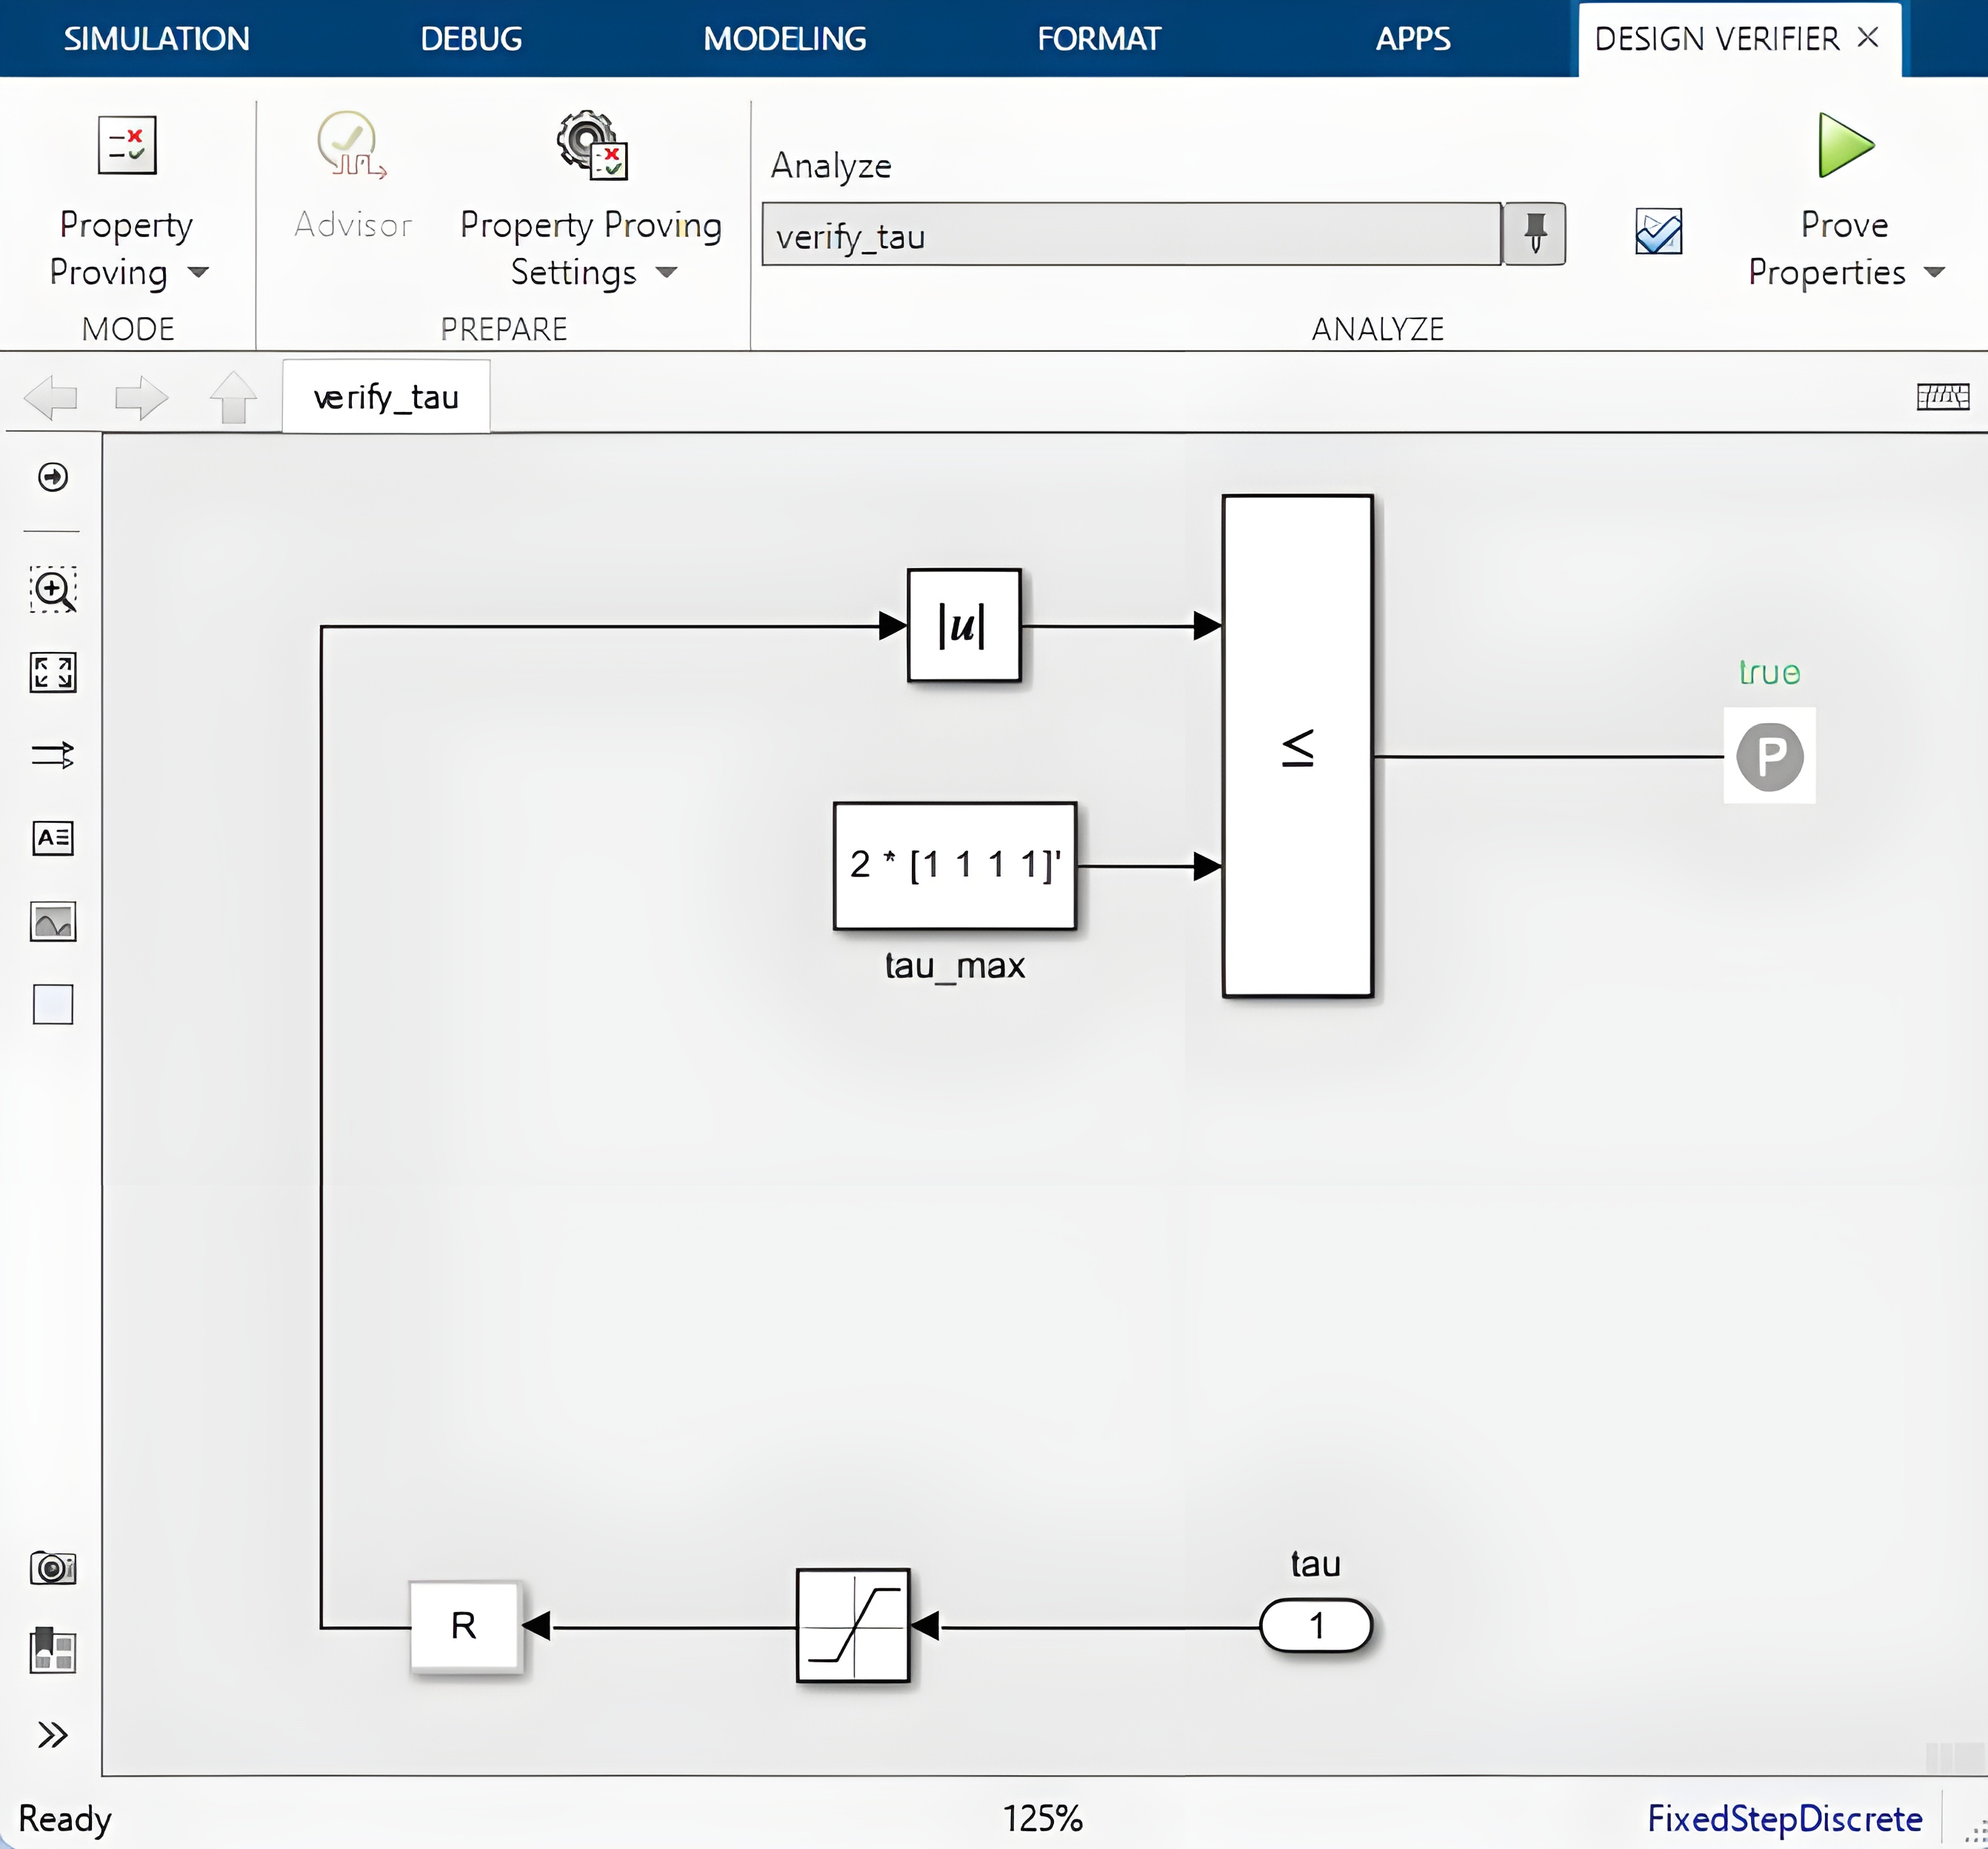
\includegraphics[width=\linewidth]{Figures/verify_tau_slx.png}
	\caption{Verification model for Simulink Design Verifier (\texttt{verify\_tau.slx}). The torque command $\tau$
  is an unconstrained input and passes through a saturation block with the limits $\pm\tau_{\max}$. A relational
  operator compares the absolute saturated torques with $\tau_{\max} = 2\,\mathrm{N\,m}$, and a proof objective
  (P) requires this comparison to be true.}
	\label{fig:verify_tau}
\end{figure}

\textbf{Scope of the Safety Components.} The mechanisms above cover a defined set of properties, namely
collision events, joint-limit events, bounded torques, and physical consistency through the momentum
check. Only the torque bound is checked formally. The collision monitor and the joint-limit monitor are
implemented in MATLAB Function blocks that compare distances and joint angles with thresholds at runtime.
They detect violations and terminate the episode but do not prove their absence. Other properties, such
as task completion within a time bound or formal stability margins, are not verified. Neither
closed-loop stability, task completion, nor collision avoidance over all possible trajectories of the
full nonlinear Simscape model is formally verified. A complete formal specification of the mission, for
example temporal-logic specifications such as ``the robot shall accomplish $X$ without $Y$ happening'',
would be considerably more complex and is beyond the scope of this work.

This work targets the safety properties that are considered most relevant for the task. Within this
scope, the runtime monitors terminated episodes that would have violated a monitored property and
penalized the corresponding actions. For TRPO and the optimized PPO agent, no violations of the monitored
constraints were observed in any evaluation episode. The other agents violated a monitored constraint in
part of their runs, and the monitors terminated these episodes. This is empirical evidence for the tested
initial states and reference trajectories, not a guarantee over all reachable states.

\textbf{Computational Overhead and Scalability.} The momentum observer and the joint-limit monitor
consist of simple algebraic operations over the link states and scale as
$\mathcal{O}(n_{\mathrm{links}})$ per time step. The pairwise distance check of the collision monitor
scales as $\mathcal{O}(n_{\mathrm{links}}^2)$. For the 4-DOF arm considered here, this overhead is small
compared with the physics simulation itself. End-to-end training times, including the full safety stack,
are reported as metric $T_2$ in \cref{tab:kpi_comp}. They range from about 7 minutes (PG) to 35 minutes
(SAC) for 1000 episodes on a standard workstation (AMD Ryzen 7 7700, 32\,GB RAM), with six training runs
executed in parallel. For onboard deployment, only the learned policy network needs to execute in the
control loop. The default and the optimized PPO agents use a compact policy network with two hidden
layers of 128 units and about $2.1 \times 10^{4}$ parameters. This is well below the memory footprint of
typical perception networks deployed on space-qualified hardware. At the 10\,Hz control rate used here, a
single forward pass through this network requires about $2 \times 10^{4}$ multiply-accumulate operations
per step. This load appears compatible with the throughput of modern space-qualified embedded processors,
for example ARM Cortex-A or LEON-class CPUs with a hardware floating-point unit. The safety monitors can
be retained as lightweight parallel watchdog processes or reduced to the most safety-critical checks
(torque saturation and joint-limit monitor) with little additional computation. This modular structure
may simplify the transfer to resource-constrained onboard systems.

In summary, the runtime safety monitors integrated into the learning process terminated unsafe simulated states
during the exploratory phase of training and shaped the agent's behavior by penalizing unsafe actions. The agent
therefore learns under runtime monitoring of the selected constraints. This combination of monitored runtime
constraints and penalty-driven learning is one approach to training deep RL policies in safety-critical domains
such as space robotics, in which unconstrained trial-and-error exploration is not admissible. The next section
analyzes the performance of the six RL agents under these conditions.

\begin{figure}[!b]
	\centering
	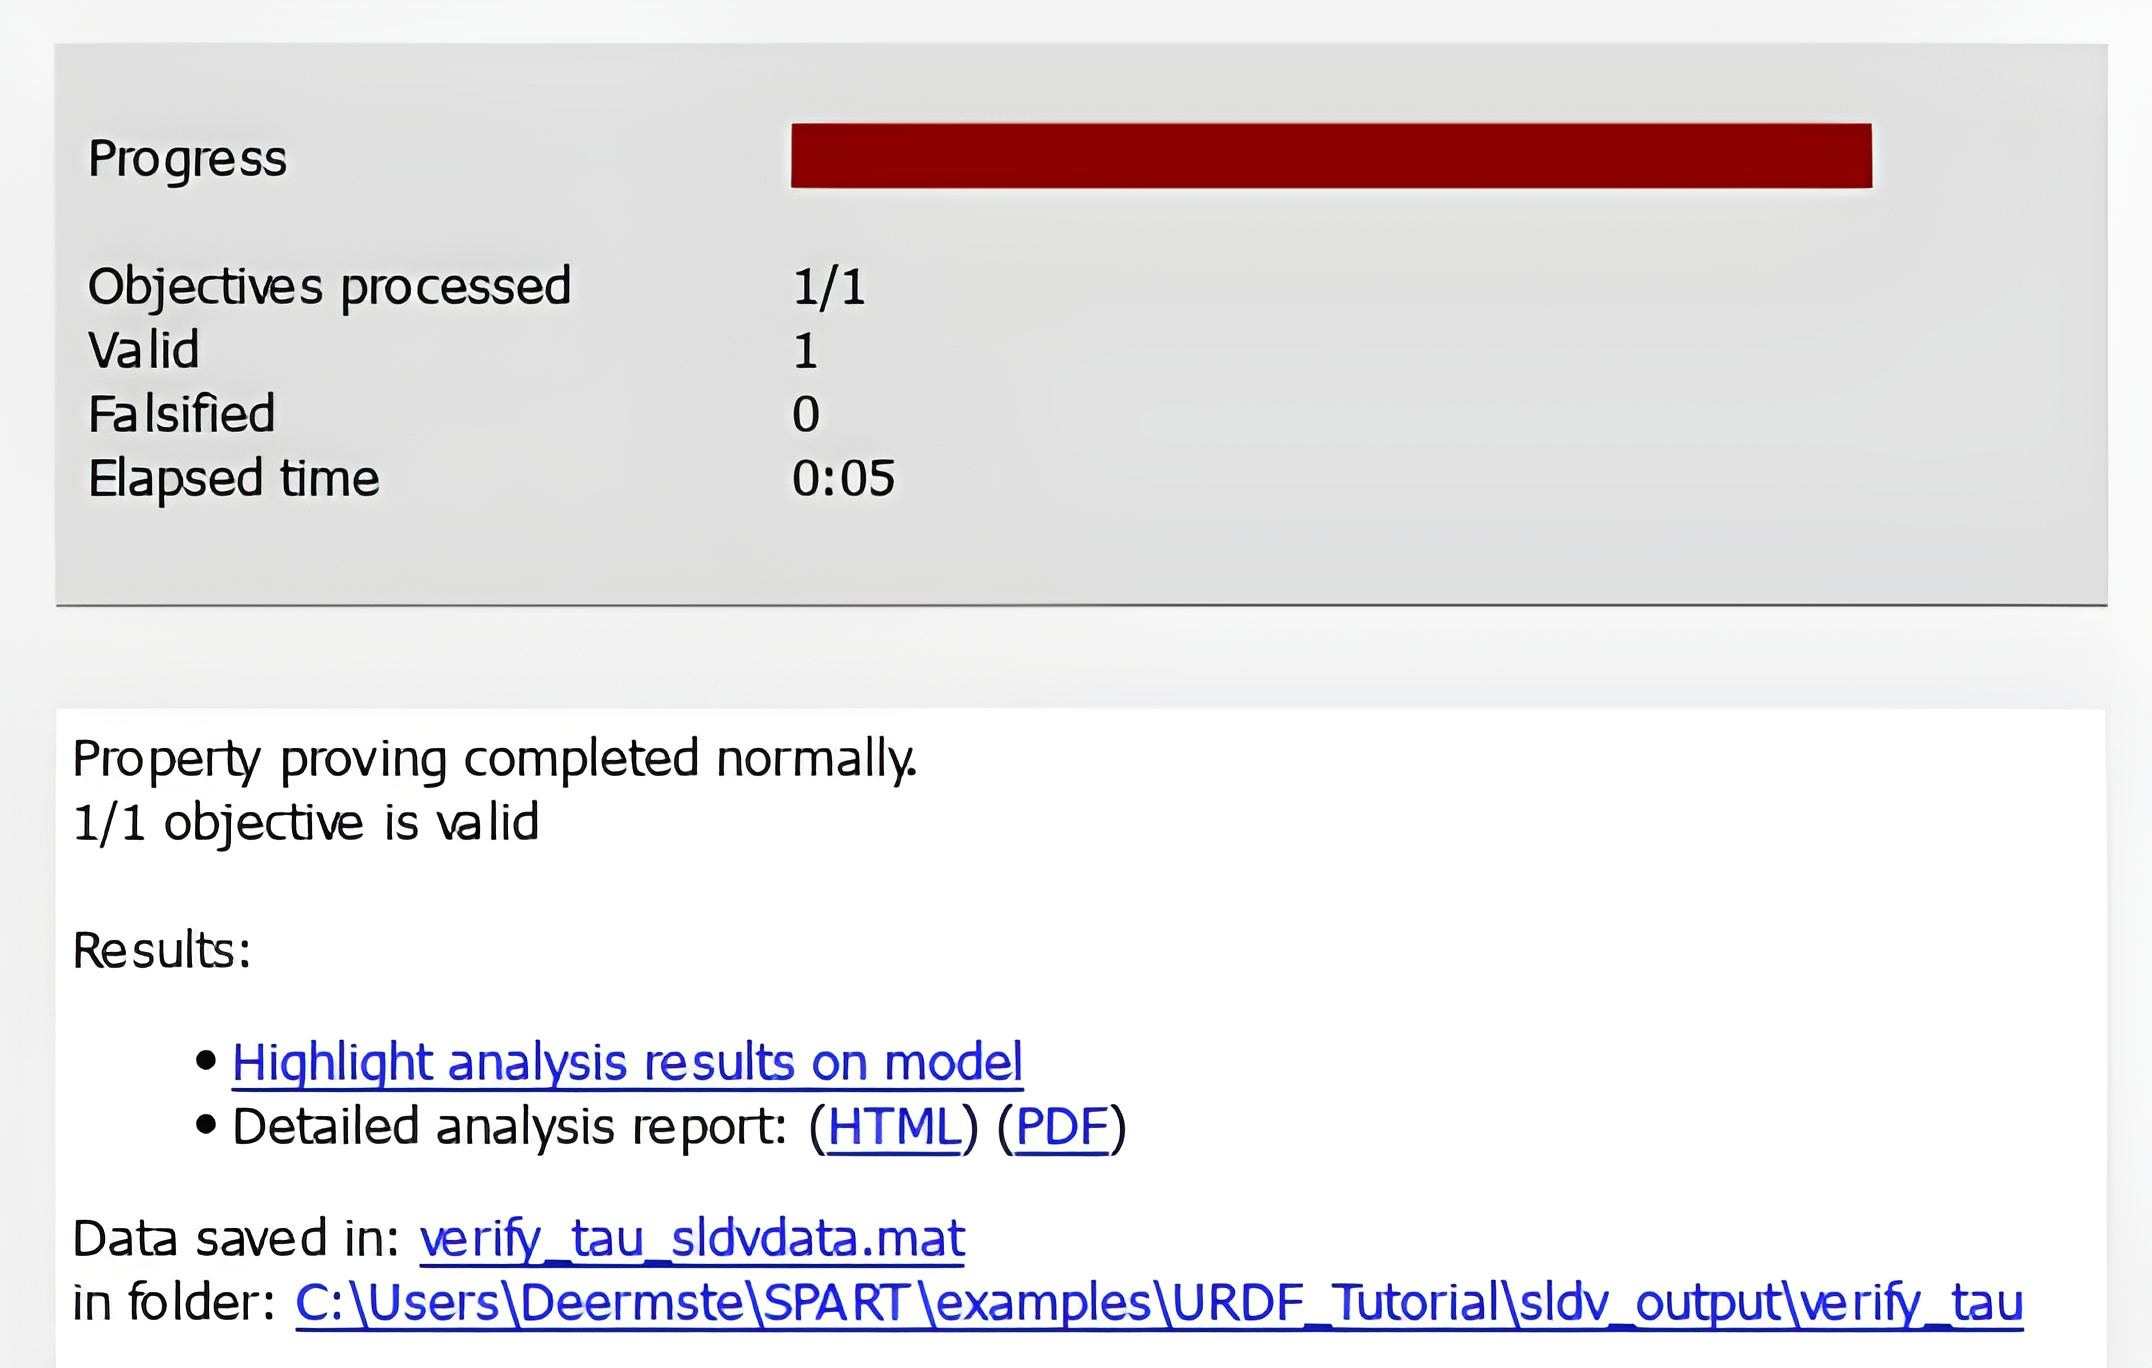
\includegraphics[width=\linewidth]{Figures/verify_tau_reslult.png}
	\caption{Result of Simulink Design Verifier for the torque-bound property. The proof objective of
  \cref{fig:verify_tau} is valid for any value of the input $\tau$, and no counterexample was found. The result
  covers only the saturation of the actuation path, not the policy network, the plant, or other properties.}
	\label{fig:verify_tau_result}
\end{figure}

\section{Comparison of Continuous RL Agents} \label{comparison}
This section compares six continuous-action RL algorithms from three families on the same task
and environment. The following algorithms are considered:

\begin{itemize}
  \item \textit{Policy Gradient (PG).} The REINFORCE algorithm (Monte Carlo policy gradient) with a learned
  state-value function as baseline \cite{b7,b21}. It is included as the simplest policy-gradient method,
  without a trust region or clipping of the policy updates.
  \item \textit{Proximal Policy Optimization (PPO).} A policy-gradient method that uses a clipped
probability-ratio surrogate to bound policy updates \cite{b15}.
  \item \textit{Trust Region Policy Optimization (TRPO).} A policy-gradient method that enforces a trust-region
constraint based on the Kullback--Leibler divergence at each update. The constrained optimization step incurs
a higher per-update computational cost than PPO \cite{b14}.
  \item \textit{Deep Deterministic Policy Gradient (DDPG).} An off-policy actor-critic algorithm with a
deterministic policy and target networks. DDPG jointly learns a $Q$-function and a policy and
is sensitive to hyperparameter choices \cite{b16}.
  \item \textit{Twin Delayed DDPG (TD3).} A variant of DDPG that uses two critic networks
  to reduce overestimation bias and delays policy updates relative to value updates \cite{b17}.
  \item \textit{Soft Actor-Critic (SAC).} An off-policy actor-critic algorithm with a stochastic policy and an
  entropy term in the objective. This entropy regularization promotes exploration but increases the per-step
  computational cost relative to deterministic methods \cite{b18}.
\end{itemize}

The six algorithms cover the on-policy/off-policy and deterministic/stochastic axes, as well as a range
of update rules. Given the strong base--manipulator coupling and the safety constraints, methods with
constrained or clipped policy updates (PPO, TRPO) are expected to provide more stable training
than algorithms without such constraints (PG, DDPG). The off-policy actor-critic methods (DDPG, TD3, SAC)
may achieve comparable performance but are typically more sensitive to hyperparameter selection.

\begin{table}[!t]
\centering
\caption{Classification of the evaluated reinforcement learning algorithms.}
\label{tab:on_off_policy}
\begin{tabular}{ll}
\toprule
\textbf{Algorithm} & \textbf{Policy Type} \\
\midrule
Policy Gradient (PG) & On-policy \\
Proximal Policy Optimization (PPO) & On-policy  \\
Trust Region Policy Optimization (TRPO) & On-policy  \\
Deep Deterministic Policy Gradient (DDPG) & Off-policy  \\
Twin Delayed DDPG (TD3) & Off-policy  \\
Soft Actor-Critic (SAC) & Off-policy  \\
\bottomrule
\end{tabular}
\end{table}
On-policy methods (PG, PPO, TRPO) update the policy only from data generated by the
current policy, which typically leads to stable but less sample-efficient learning. Off-policy methods (DDPG,
TD3, SAC) reuse experience stored in a replay buffer, which improves sample efficiency at
the cost of higher sensitivity to hyperparameters~\cite{b2,b7}.

\textbf{Training Setup.} All experiments were performed on a workstation with an AMD Ryzen 7 7700
processor and 32\,GB of RAM, using MATLAB R2026a with the Reinforcement Learning Toolbox and Simscape
Multibody. All six agents use the default hyperparameters and the default networks of the Reinforcement
Learning Toolbox with two hidden layers of 128 ReLU units. Only the sample time is set to
$\Delta t$. \cref{tab:hyperparameters} lists the resulting values. The reward function, the network size,
and the training budget are the same for all agents, and no agent is tuned individually. Observed
differences therefore reflect the algorithms together with their default hyperparameters. PPO was further
tuned in a subsequent step. In the main comparison, PPO uses its default configuration. Each
configuration was trained with ten seeds for 1000 episodes, and the policy after the last episode was
evaluated.

\begin{table*}[!t]
\centering
\caption{Hyperparameters of the benchmarked agents. The six default agents use the default values of the
Reinforcement Learning Toolbox (R2026a). All agents act every $\Delta t = 0.1\,\mathrm{s}$ and use
networks with two hidden layers of 128 ReLU units. In contrast to the default PPO agent, the policy mean
of the optimized PPO agent has no tanh output layer. $\alpha_a$ and $\alpha_c$ denote the actor and
critic learning rates.}
\label{tab:hyperparameters}
\begin{tabular}{lcccccl}
\toprule
\textbf{Agent} & $\alpha_a$ & $\alpha_c$ & $\gamma$ & \textbf{Experience} & \textbf{Mini-batch} & \textbf{Further settings} \\
\midrule
PG & $10^{-2}$ & $10^{-2}$ & 0.99 & 1 episode & -- & entropy weight 0, critic as baseline \\
PPO (default) & $10^{-2}$ & $10^{-2}$ & 0.99 & horizon 512 & 128 & 3 epochs, clip 0.2, entropy 0.01, GAE 0.95 \\
TRPO & -- & $10^{-2}$ & 0.99 & horizon 512 & 128 & KL limit 0.01, entropy 0.01, GAE 0.95 \\
DDPG & $10^{-2}$ & $10^{-2}$ & 0.99 & buffer $10^4$ & 64 & target smoothing 0.001, OU noise $\sigma = 0.3$ \\
TD3 & $10^{-2}$ & $10^{-2}$ & 0.99 & buffer $10^4$ & 64 & target smoothing 0.005, noise $\sigma = 0.32$, policy delay 2 \\
SAC & $10^{-2}$ & $10^{-2}$ & 0.99 & buffer $10^4$ & 64 & target smoothing 0.001 \\
\midrule
PPO (optimized) & $10^{-3}$ & $5\!\times\!10^{-4}$ & 0.995 & horizon 1024 & 256 & 10 epochs, clip 0.2, entropy 0.001, GAE 0.95, gradient threshold 1 \\
\bottomrule
\end{tabular}
\end{table*}


\textbf{Evaluation Protocol.} The agents were evaluated with the protocol of \cref{RL}. Each of the 60
default runs was evaluated on the same 31 initial states. A run counts as successful when none of its
evaluation episodes was terminated by a monitor. \cref{tab:robustness_seeds} reports the number of
successful runs and the abort rate over all runs. \cref{tab:kpi_comp} reports the KPIs over the
successful runs only.

\begin{table}[!t]
\centering
\caption{Success of the default agents over ten training runs each. A run is successful when none of its
31 evaluation episodes is terminated by a monitor. The abort rate is the share of terminated episodes among
the 310 evaluation episodes of an agent. The column ``Aborts by contact'' gives the share of these
terminated episodes that ended with a detected contact. The remaining terminations were caused by
joint-limit violations. The last column gives the $p$-value of Fisher's exact test on the number of
successful runs against TRPO, Holm-corrected over the five compared agents.}
\label{tab:robustness_seeds}
\renewcommand{\arraystretch}{1.2}
\begin{tabular}{lcccc}
\toprule
\textbf{Agent} & \textbf{Successful} & \textbf{Abort} & \textbf{Aborts by} & $\boldsymbol{p}$ \\
 & \textbf{runs} & \textbf{rate} & \textbf{contact} & \textbf{vs.\ TRPO} \\
\midrule
TRPO & 10/10 & 0.0\% & -- & -- \\
SAC & 6/10 & 40.0\% & 0.0\% & 0.087 \\
TD3 & 5/10 & 48.4\% & 24.7\% & 0.065 \\
DDPG & 4/10 & 51.6\% & 22.5\% & 0.033 \\
PPO & 3/10 & 70.0\% & 14.3\% & 0.012 \\
PG & 2/10 & 80.0\% & 1.6\% & 0.0036 \\
\bottomrule
\end{tabular}
\end{table}

\textbf{Success Across Seeds.} The number of successful runs ranged from two to ten out of ten
(\cref{tab:robustness_seeds}). TRPO completed all ten runs without a terminated evaluation episode.
SAC, TD3, and DDPG succeeded in four to six runs, the default PPO agent in three, and PG in two. In
27 of the 30 failed runs, all 31 evaluation episodes were terminated. A failed run therefore reflects a
systematic property of the learned policy. Most terminations were caused by joint-limit violations.
Contacts between robot bodies occurred only in runs of TD3, DDPG, PPO, and PG. Compared with TRPO, the
number of successful runs was significantly lower for PG, PPO, and DDPG (Fisher's exact test,
Holm-corrected $p \le 0.033$). The differences to TD3 and SAC were not significant with ten runs per
agent.

\begin{table*}[!t]
\centering
\caption{Performance of the successful runs of the default agents on the circular path. The first row gives
the number of successful runs out of ten. All other values are the mean and the standard deviation over the
successful runs of an agent. The collision rate $K_5$ and the joint limit violation rate $K_6$ are zero for
every successful run and are omitted.}
\label{tab:kpi_comp}
\renewcommand{\arraystretch}{1.2}
\setlength{\tabcolsep}{2.4pt}
\footnotesize
\begin{tabular}{lcccccc}
\toprule
\textbf{Metric (KPI)} & \textbf{TRPO} & \textbf{SAC} & \textbf{TD3} & \textbf{DDPG} & \textbf{PPO} &
  \textbf{PG} \\
\midrule
Successful runs & 10/10 & 6/10 & 5/10 & 4/10 & 3/10 & 2/10 \\
Mean Episodic Return ($K_1$) & $-0.44 \pm 0.55$ & $-7.42 \pm 3.22$ & $-3.52 \pm 1.28$ &
  $-12.24 \pm 9.38$ & $-0.72 \pm 0.12$ & $-0.53 \pm 0.07$ \\
Mean Squared EE Position Error ($K_2$) & $0.0145 \pm 0.0196$ & $0.2168 \pm 0.1098$ &
  $0.0886 \pm 0.0560$ & $0.1599 \pm 0.0919$ & $0.0134 \pm 0.0081$ & $0.0177 \pm 0.0036$ \\
Maximum EE Position Error ($K_3$) & $0.229 \pm 0.095$ & $0.975 \pm 0.225$ & $0.609 \pm 0.248$ &
  $1.001 \pm 0.504$ & $0.215 \pm 0.040$ & $0.262 \pm 0.004$ \\
Mean Base Orientation Error ($K_4$) & $0.026 \pm 0.009$ & $0.144 \pm 0.092$ & $0.098 \pm 0.080$ &
  $0.353 \pm 0.171$ & $0.050 \pm 0.014$ & $0.030 \pm 0.011$ \\
Control Smoothness ($K_7$, Jerk) & $0.0098 \pm 0.0017$ & $0.197 \pm 0.222$ & $0.515 \pm 0.213$ &
  $0.549 \pm 0.193$ & $0.383 \pm 0.068$ & $0.0056 \pm 0.0008$ \\
Mean Base Angular Velocity ($K_8$) & $0.017 \pm 0.008$ & $0.045 \pm 0.022$ & $0.047 \pm 0.012$ &
  $0.097 \pm 0.054$ & $0.031 \pm 0.007$ & $0.017 \pm 0.005$ \\
Energy Consumption ($K_9$) & $2.00 \pm 0.78$ & $8.65 \pm 7.20$ & $19.3 \pm 12.5$ & $16.3 \pm 6.5$ &
  $12.4 \pm 9.7$ & $1.49 \pm 0.50$ \\
Reward Std.\ (Late Training, $T_1$) & $0.26 \pm 0.18$ & $13.9 \pm 5.2$ & $16.9 \pm 7.5$ &
  $20.0 \pm 4.3$ & $1.23 \pm 0.58$ & $0.25 \pm 0.08$ \\
Training Time ($T_2$, min) & $11.3 \pm 0.7$ & $35.2 \pm 0.4$ & $29.1 \pm 1.4$ & $24.3 \pm 0.2$ &
  $8.4 \pm 0.7$ & $6.9 \pm 1.3$ \\
\bottomrule
\end{tabular}
\end{table*}

\begin{figure*}[!t]
	\centering
	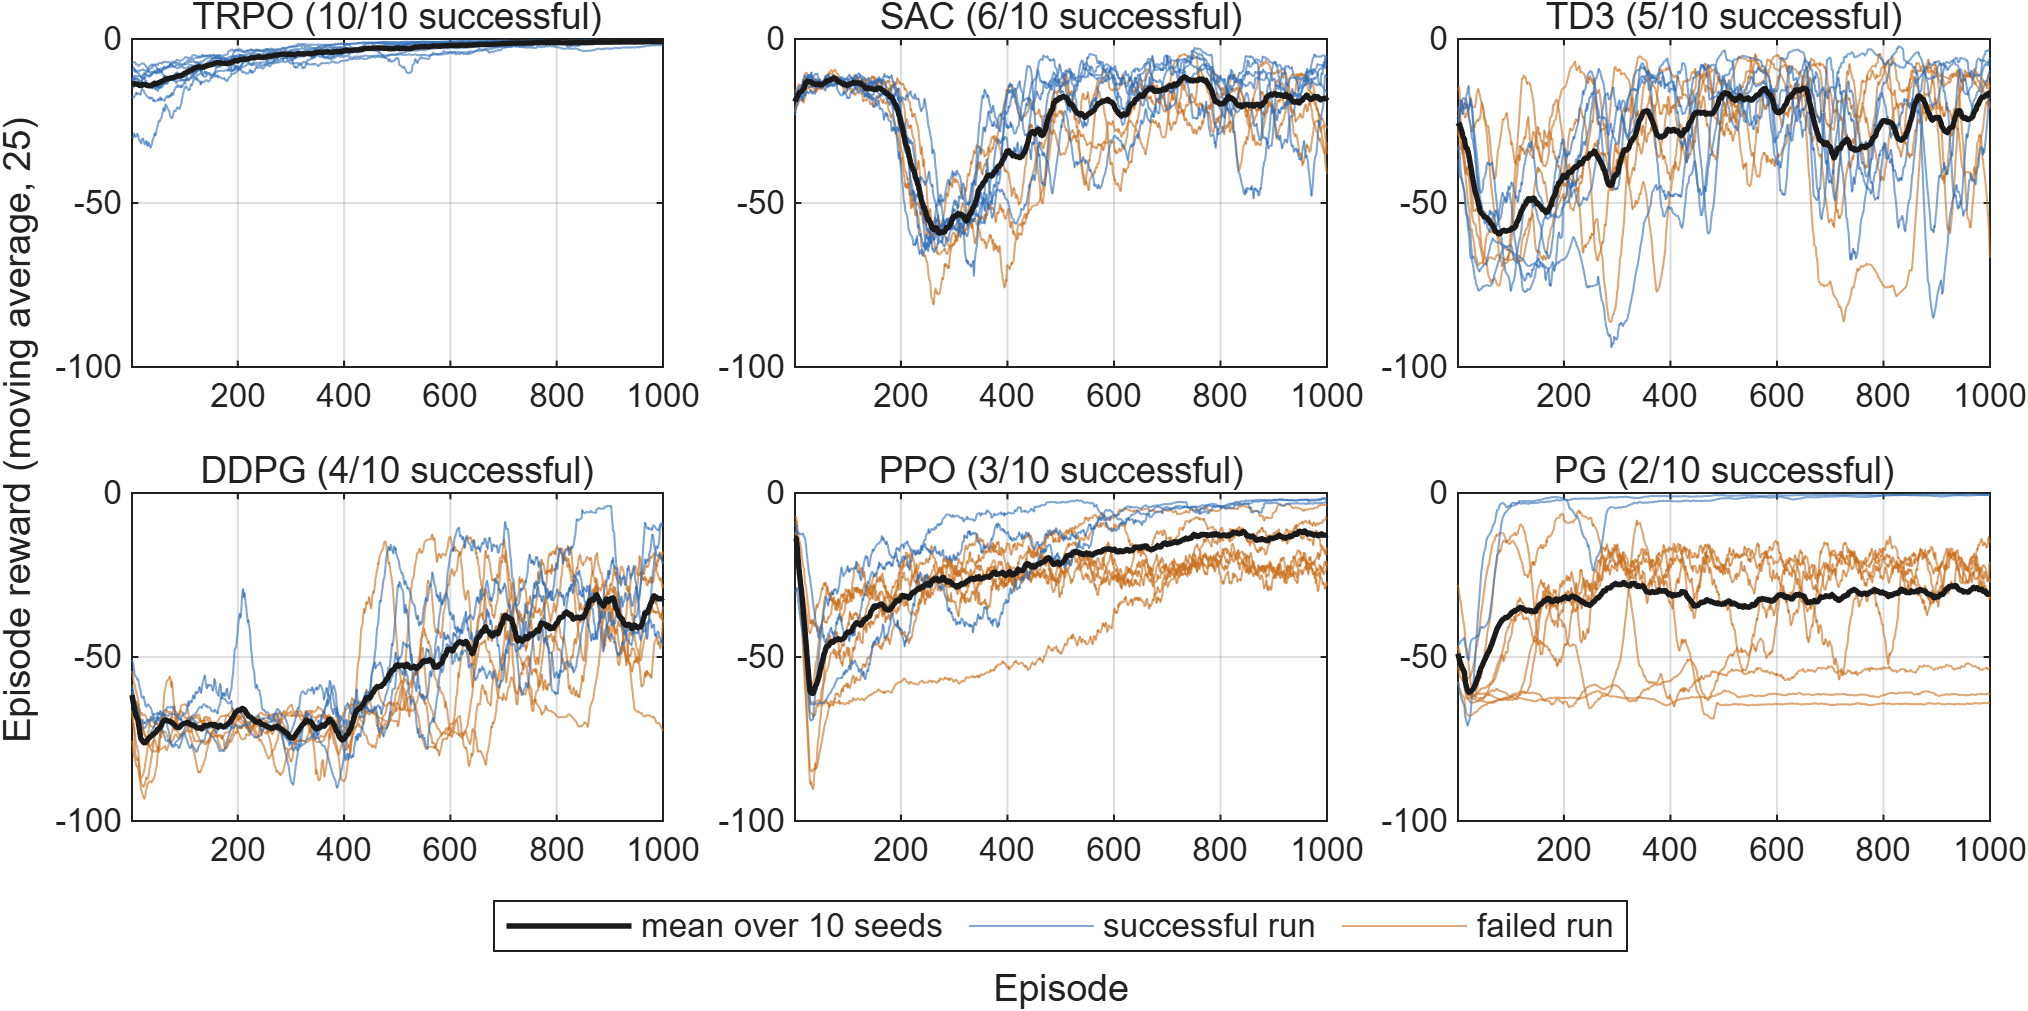
\includegraphics[width=0.9\linewidth]{Figures/trainingsverlauf_defaults.png}
	\caption{Episode rewards during training of the six default agents over ten seeds each. Each thin line
  shows one seed as a moving average over 25 episodes. Blue lines are successful runs, orange lines are
  failed runs, and the black line is the mean over the ten seeds. All panels use the same axis.}
	\label{fig:training_defaults}
\end{figure*}

\textbf{Performance of the Successful Runs.} \cref{tab:kpi_comp} summarizes the KPIs and the training
metrics of the successful runs. TRPO, PPO, and PG reached mean squared tracking errors between 0.013 and
0.018 in their successful runs. TD3, DDPG, and SAC remained between 0.089 and 0.217, although their
successful runs completed every evaluation episode. Their base orientation errors were also larger ($K_4$
between 0.098 and 0.353, compared with 0.026 for TRPO). The standard deviation of TRPO results mainly
from three of the ten runs with $K_2$ between 0.021 and 0.066 (\cref{fig:boxplot_k2}). The median of
TRPO is 0.0061.

TRPO required 11.3\,min per training run, the default PPO agent 8.4\,min, and PG 6.9\,min. The off-policy
agents required 24.3 to 35.2\,min. The standard deviation of the late-training reward was small for TRPO,
PPO, and PG ($T_1 \le 1.23$) and large for TD3, DDPG, and SAC ($T_1$ between 13.9 and 20.0). This
suggests that the off-policy agents had not settled after 1000 episodes. The learning curves in
\cref{fig:training_defaults} show the same pattern. The returns of TRPO rose toward zero in all ten runs
with a small spread between the seeds. The returns of TD3, DDPG, and SAC still fluctuated at the end of
training, in both successful and failed runs. For PG and the default PPO agent, the failed runs ended
at lower returns than the successful runs.

The control smoothness $K_7$ and the energy consumption $K_9$ separate the agents in a similar way. TRPO
and PG produced smooth torque commands ($K_7 \le 0.010$) with a low energy consumption ($K_9 \le 2.0$).
The default PPO agent tracked the path with a similar error but with a larger jerk ($K_7 = 0.383$) and
energy consumption ($K_9 = 12.4$). The off-policy agents combined larger tracking errors with $K_7$
between 0.20 and 0.55 and $K_9$ between 8.6 and 19.3.

\begin{table*}[!t]
\centering
\caption{Seed-level comparison of the successful runs of the default agents with those of TRPO. Each cell
gives the median difference $\Delta\tilde{x}$ (agent minus TRPO) with the Holm-corrected significance of a
two-sided Mann--Whitney $U$ test as superscript (${}^{***}p<0.001$, ${}^{**}p<0.01$, ${}^{*}p<0.05$,
${}^{\mathrm{n.s.}}p\geq0.05$). For $K_1$, a negative difference means a lower return than TRPO. For the
other KPIs, a positive difference means a larger error, jerk, angular velocity, or energy than TRPO. The
Holm correction covers the three tested agents for each KPI. PPO and PG are not tested because they have
fewer than four successful runs.}
\label{tab:significance}
\renewcommand{\arraystretch}{1.3}
\setlength{\tabcolsep}{5pt}
\footnotesize
\begin{tabular}{lc *{7}{r}}
\toprule
\textbf{Agent} & $\boldsymbol{n}$ & $\boldsymbol{K_1}$ & $\boldsymbol{K_2}$ & $\boldsymbol{K_3}$ &
  $\boldsymbol{K_4}$ & $\boldsymbol{K_7}$ & $\boldsymbol{K_8}$ & $\boldsymbol{K_9}$ \\
\midrule
SAC  & 6 & $-8.08^{***}$ & $+0.180^{***}$ & $+0.779^{***}$ & $+0.134^{*}$ & $+0.125^{\mathrm{n.s.}}$ &
  $+0.027^{*}$ & $+7.06^{\mathrm{n.s.}}$ \\
TD3  & 5 & $-3.07^{**}$ & $+0.085^{**}$ & $+0.387^{**}$ & $+0.046^{**}$ & $+0.532^{**}$ &
  $+0.027^{**}$ & $+18.3^{**}$ \\
DDPG & 4 & $-7.81^{**}$ & $+0.128^{**}$ & $+0.770^{**}$ & $+0.299^{**}$ & $+0.562^{**}$ &
  $+0.062^{**}$ & $+13.1^{**}$ \\
\bottomrule
\end{tabular}
\end{table*}

\textbf{Statistical Tests.} \cref{tab:significance} compares the successful runs of each default agent
with those of TRPO on the seed level. PPO and PG are not tested because they have fewer than four
successful runs. SAC, TD3, and DDPG had a significantly lower return $K_1$ and significantly larger
tracking errors $K_2$ and $K_3$ than TRPO (Holm-corrected $p \le 0.005$). Their base orientation error
$K_4$ was also significantly larger ($p = 0.031$ for SAC and $p \le 0.006$ for TD3 and DDPG).
For SAC, the differences in $K_7$ and $K_9$ were not significant.

\cref{fig:boxplots} shows the distribution of four KPIs over the successful runs, and
\cref{fig:ci_plots} shows the corresponding 95\% bootstrap confidence intervals of the mean. Both figures
include the optimized PPO agent of \cref{sec:ppo_opt} for reference.

\begin{figure*}[!t]
  \centering
  \begin{subfigure}{0.48\textwidth}
    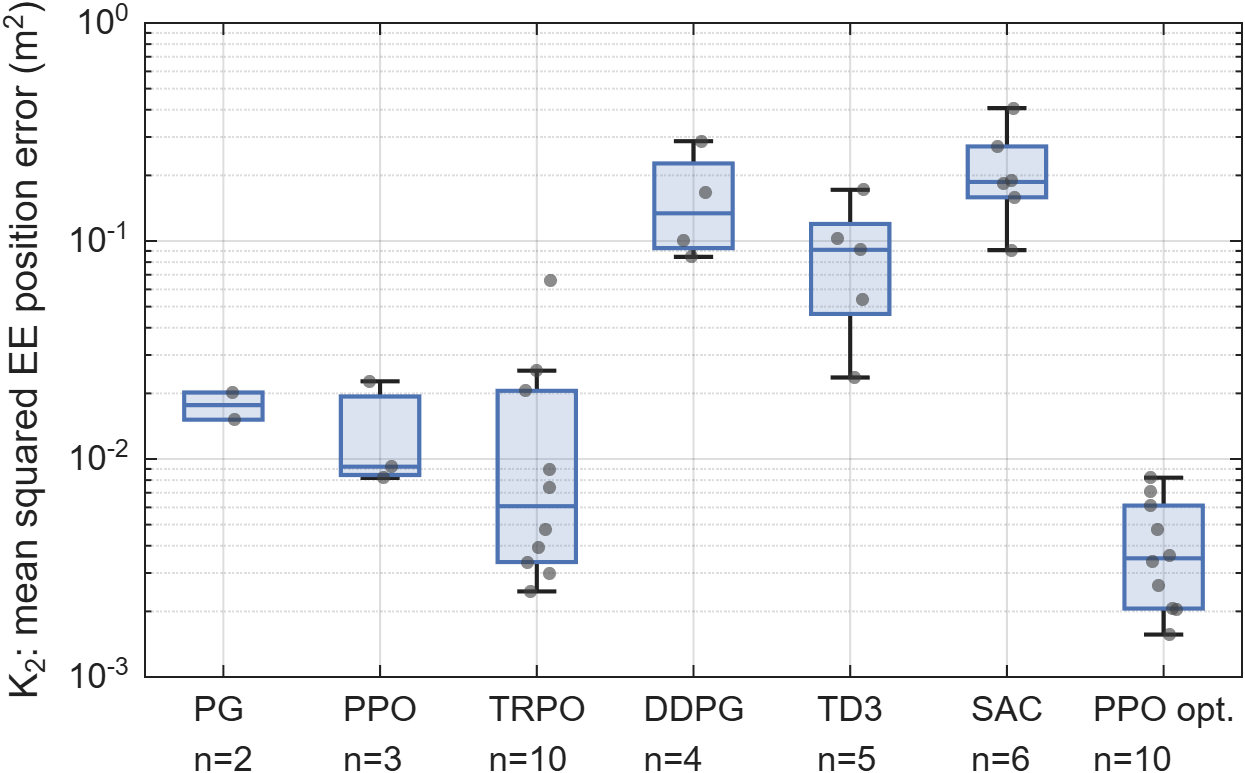
\includegraphics[width=\linewidth]{Figures/boxplot_K2.png}
    \caption{$K_2$: Mean Squared EE Position Error}
    \label{fig:boxplot_k2}
  \end{subfigure}
  \hfill
  \begin{subfigure}{0.48\textwidth}
    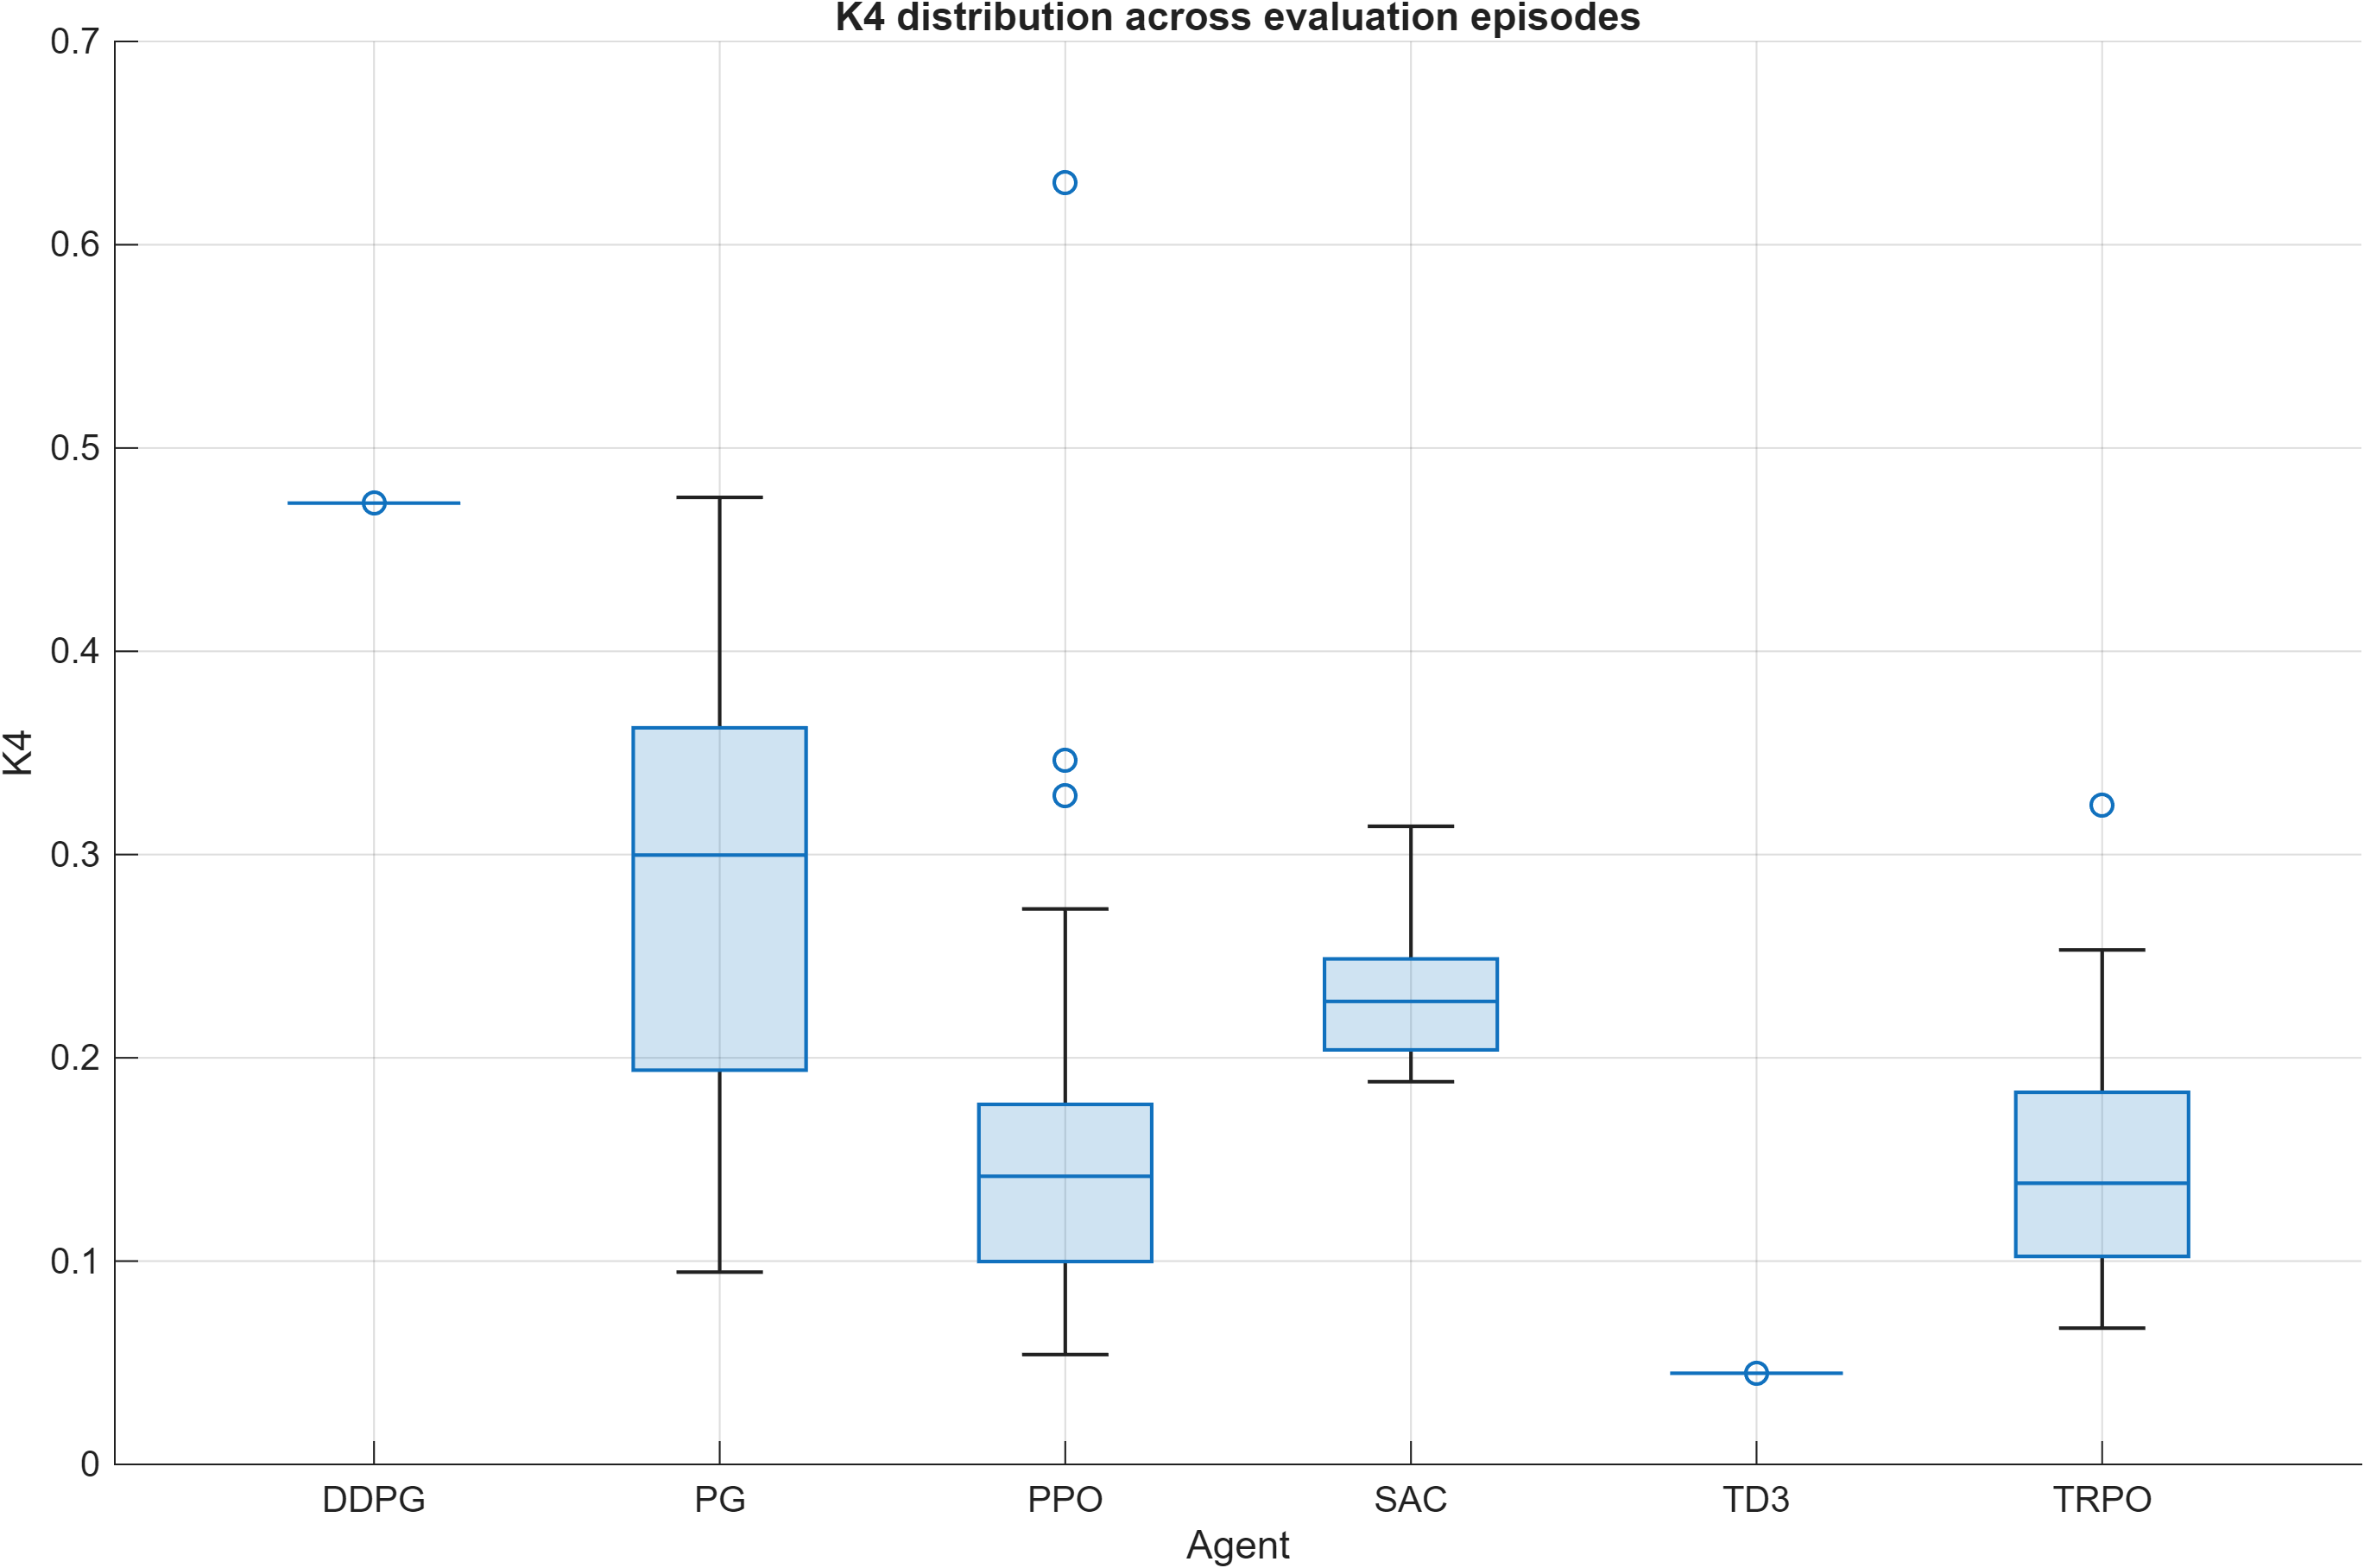
\includegraphics[width=\linewidth]{Figures/boxplot_K4.png}
    \caption{$K_4$: Mean Base Orientation Error}
    \label{fig:boxplot_k4}
  \end{subfigure}
  \\[6pt]
  \begin{subfigure}{0.48\textwidth}
    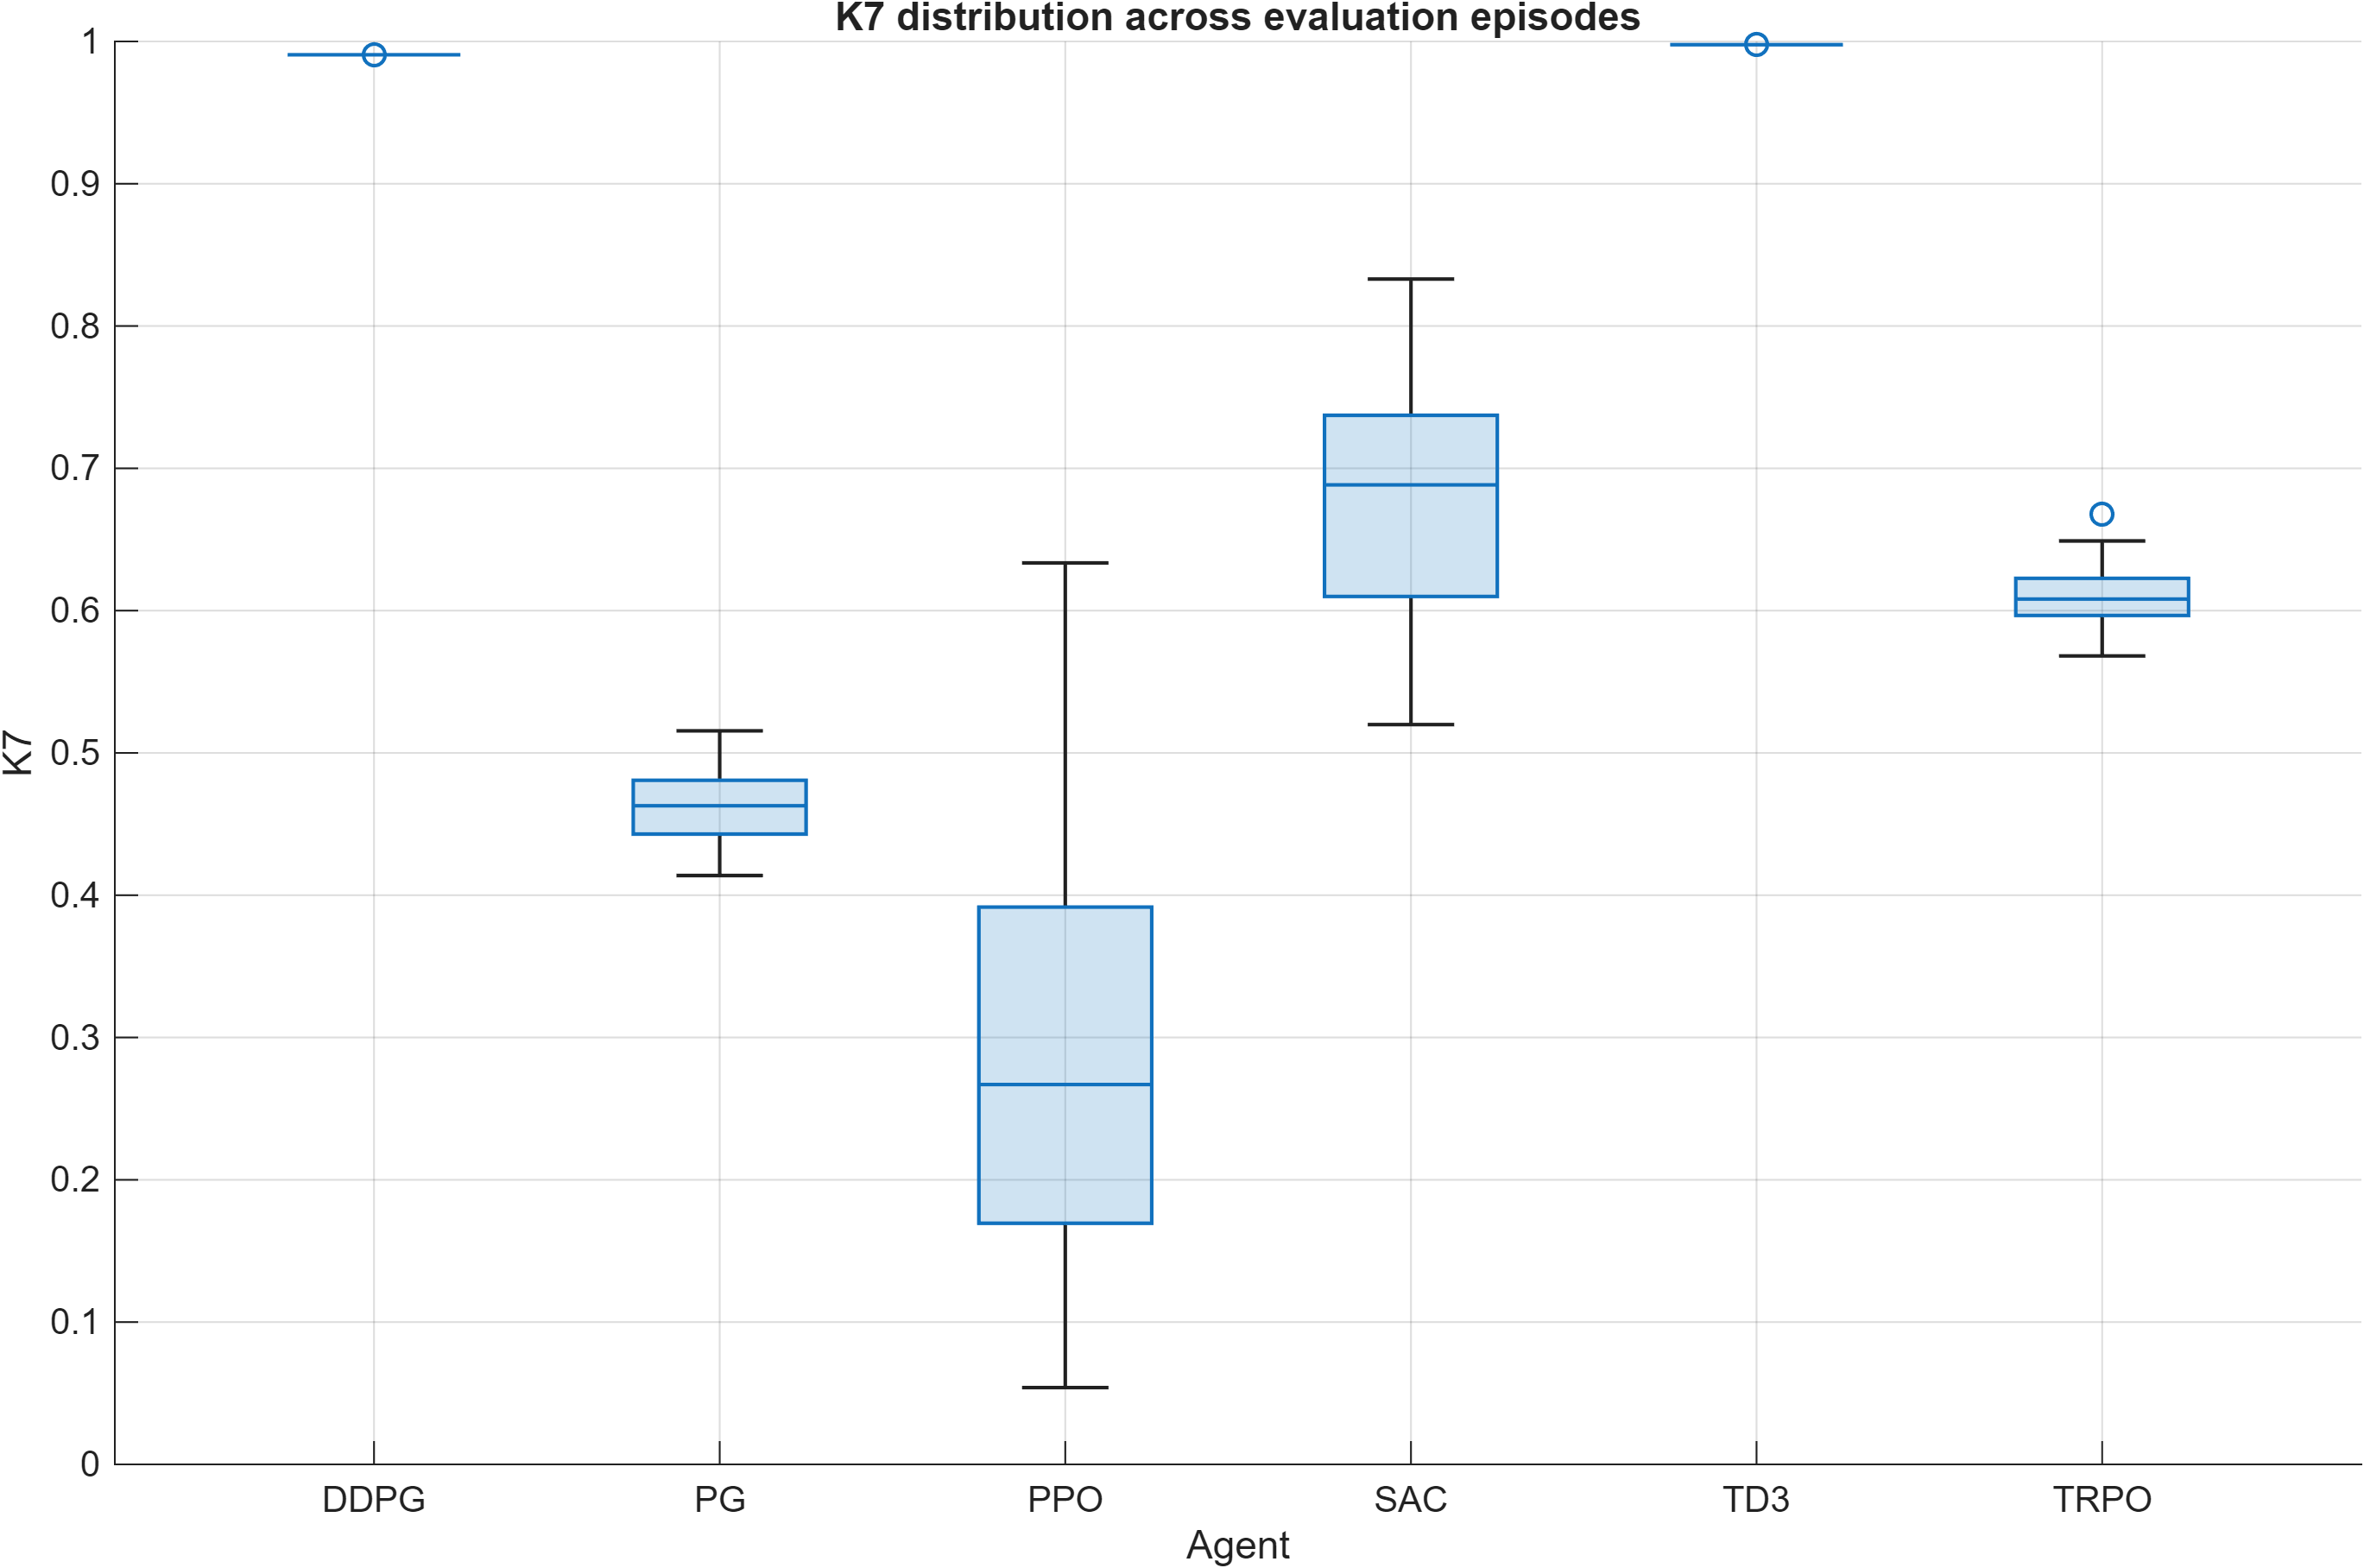
\includegraphics[width=\linewidth]{Figures/boxplot_K7.png}
    \caption{$K_7$: Control Smoothness (Jerk)}
    \label{fig:boxplot_k7}
  \end{subfigure}
  \hfill
  \begin{subfigure}{0.48\textwidth}
    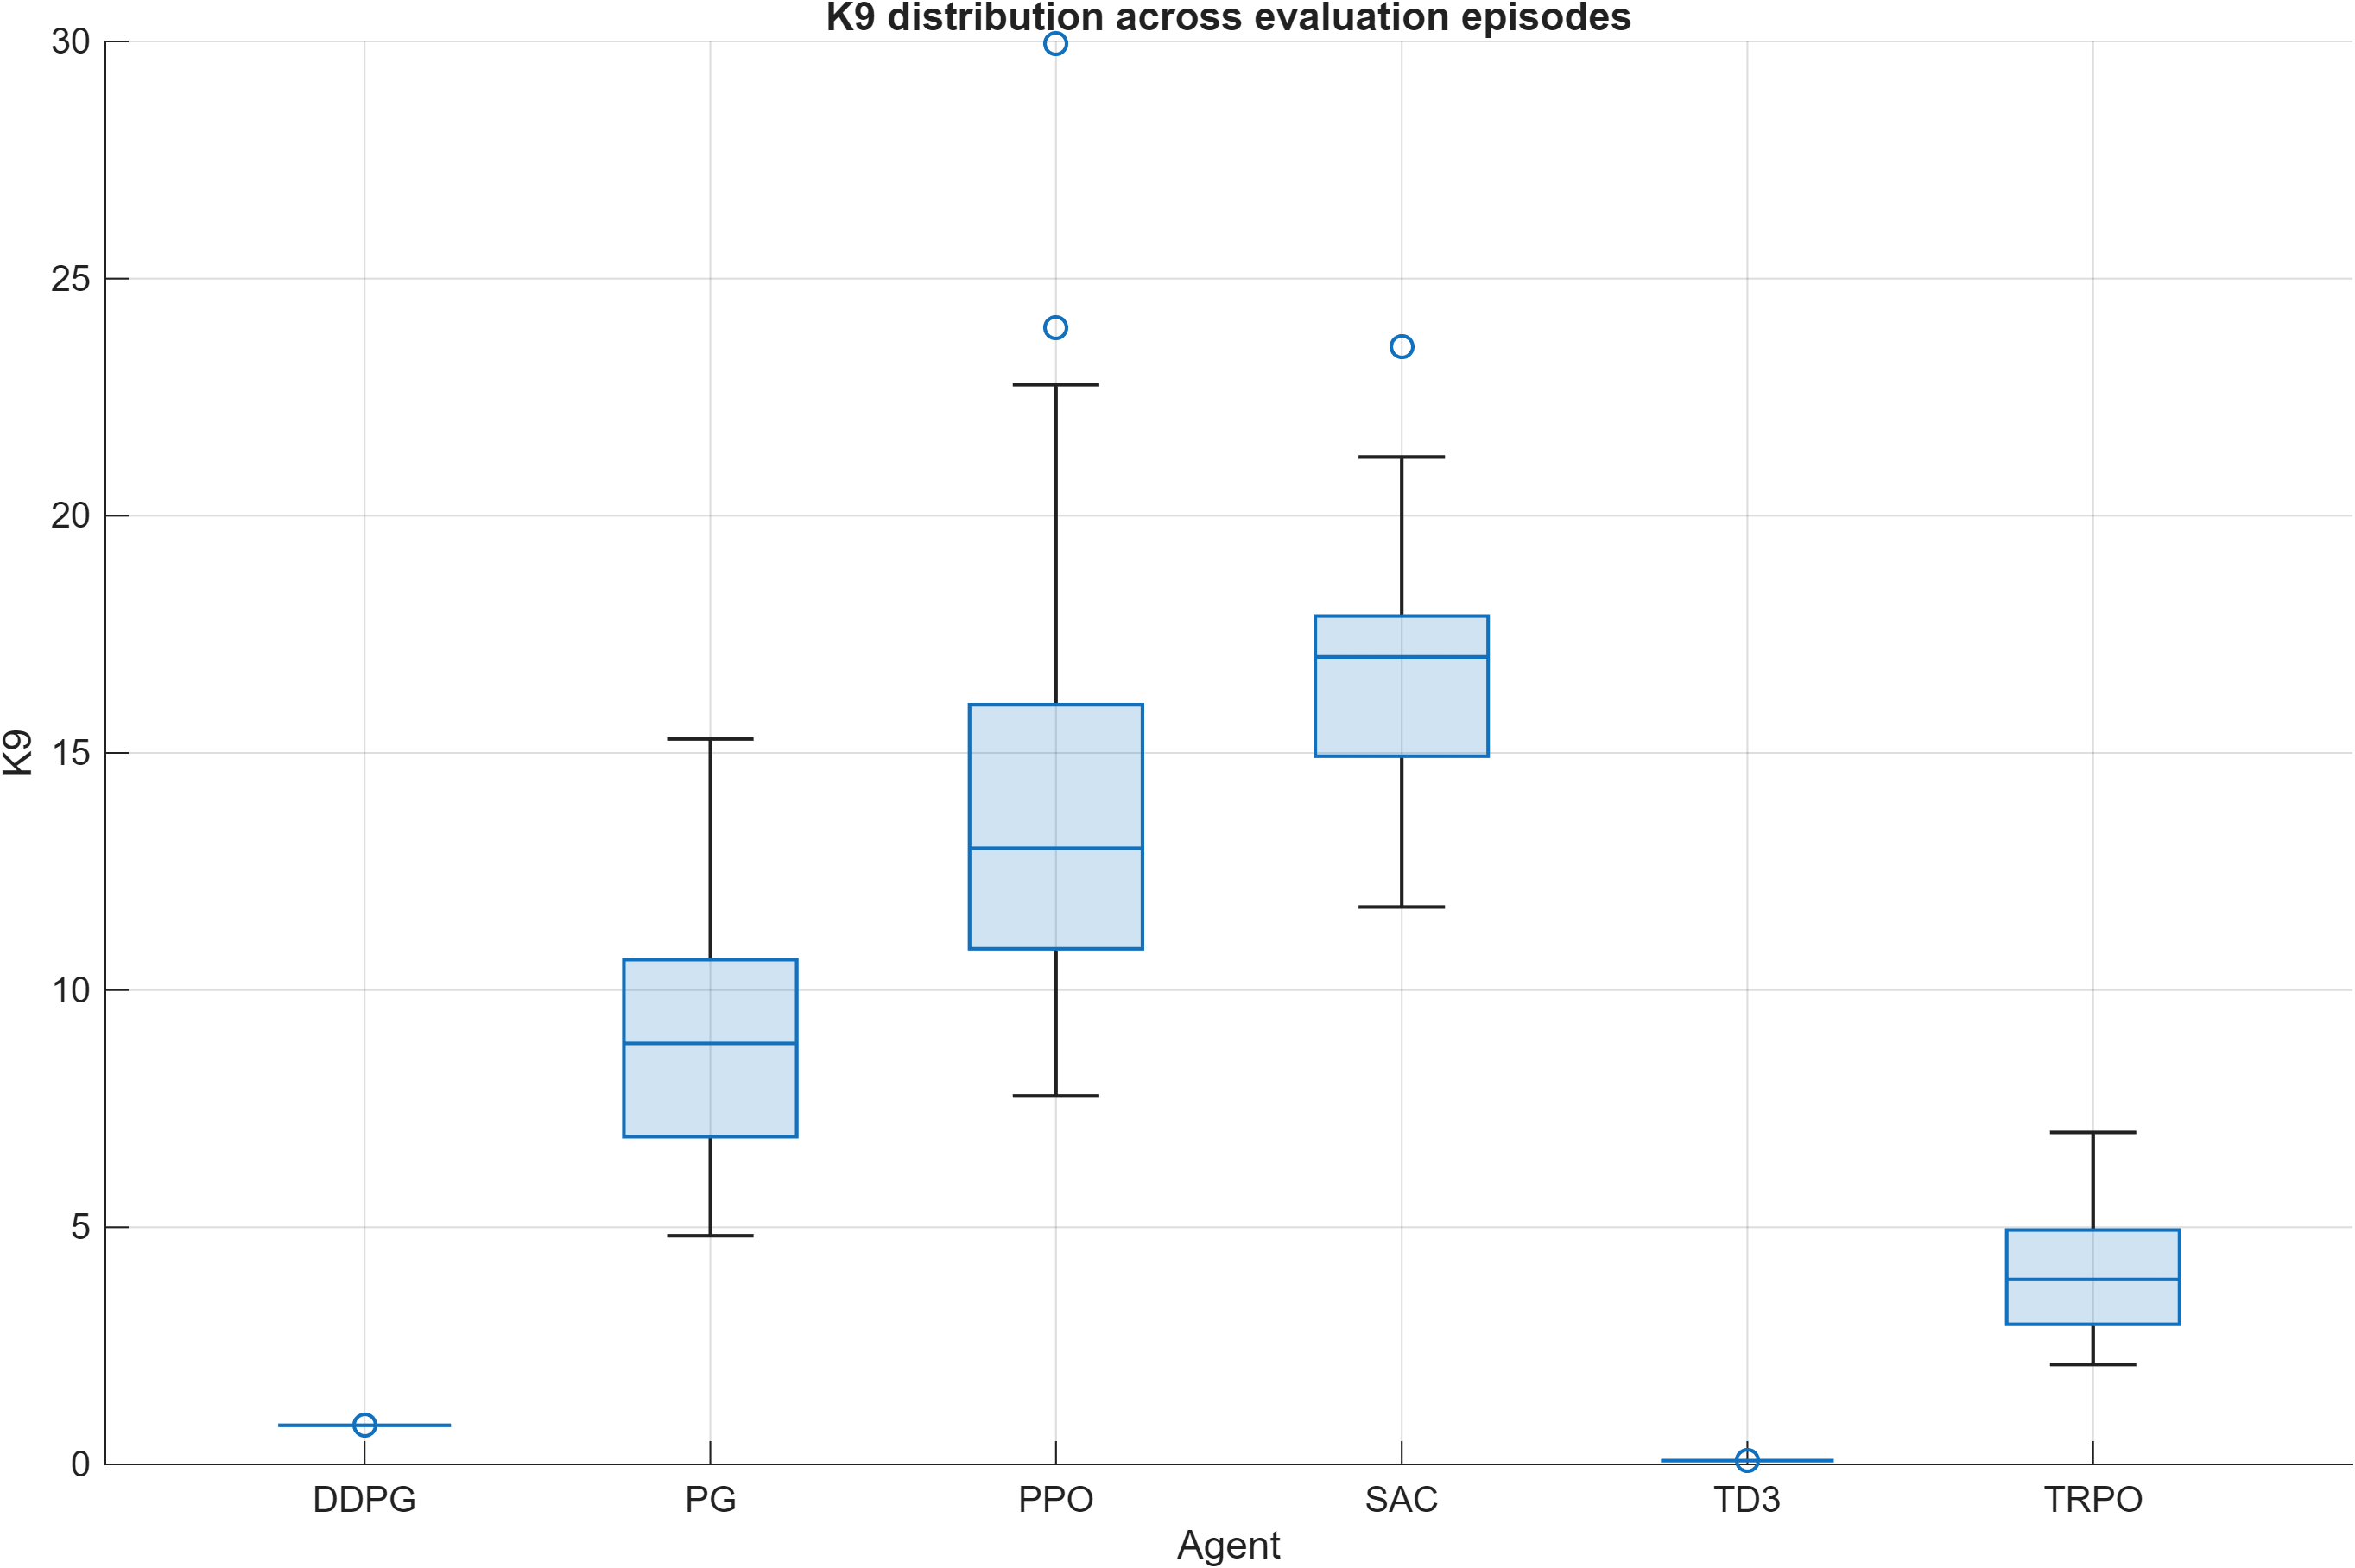
\includegraphics[width=\linewidth]{Figures/boxplot_K9.png}
    \caption{$K_9$: Energy Consumption}
    \label{fig:boxplot_k9}
  \end{subfigure}
  \caption{Distribution of selected KPIs over the successful runs of each agent. Each point is one run,
    averaged over the 30 random initial states, and the number of successful runs is given below each
    agent. Each box spans the interquartile range, and the center line marks the median. Axes are
    logarithmic where the values span more than a factor of 50. The optimized PPO agent of
    \cref{sec:ppo_opt} is included for reference.}
  \label{fig:boxplots}
\end{figure*}

\begin{figure*}[!t]
  \centering
  \begin{subfigure}{0.48\textwidth}
    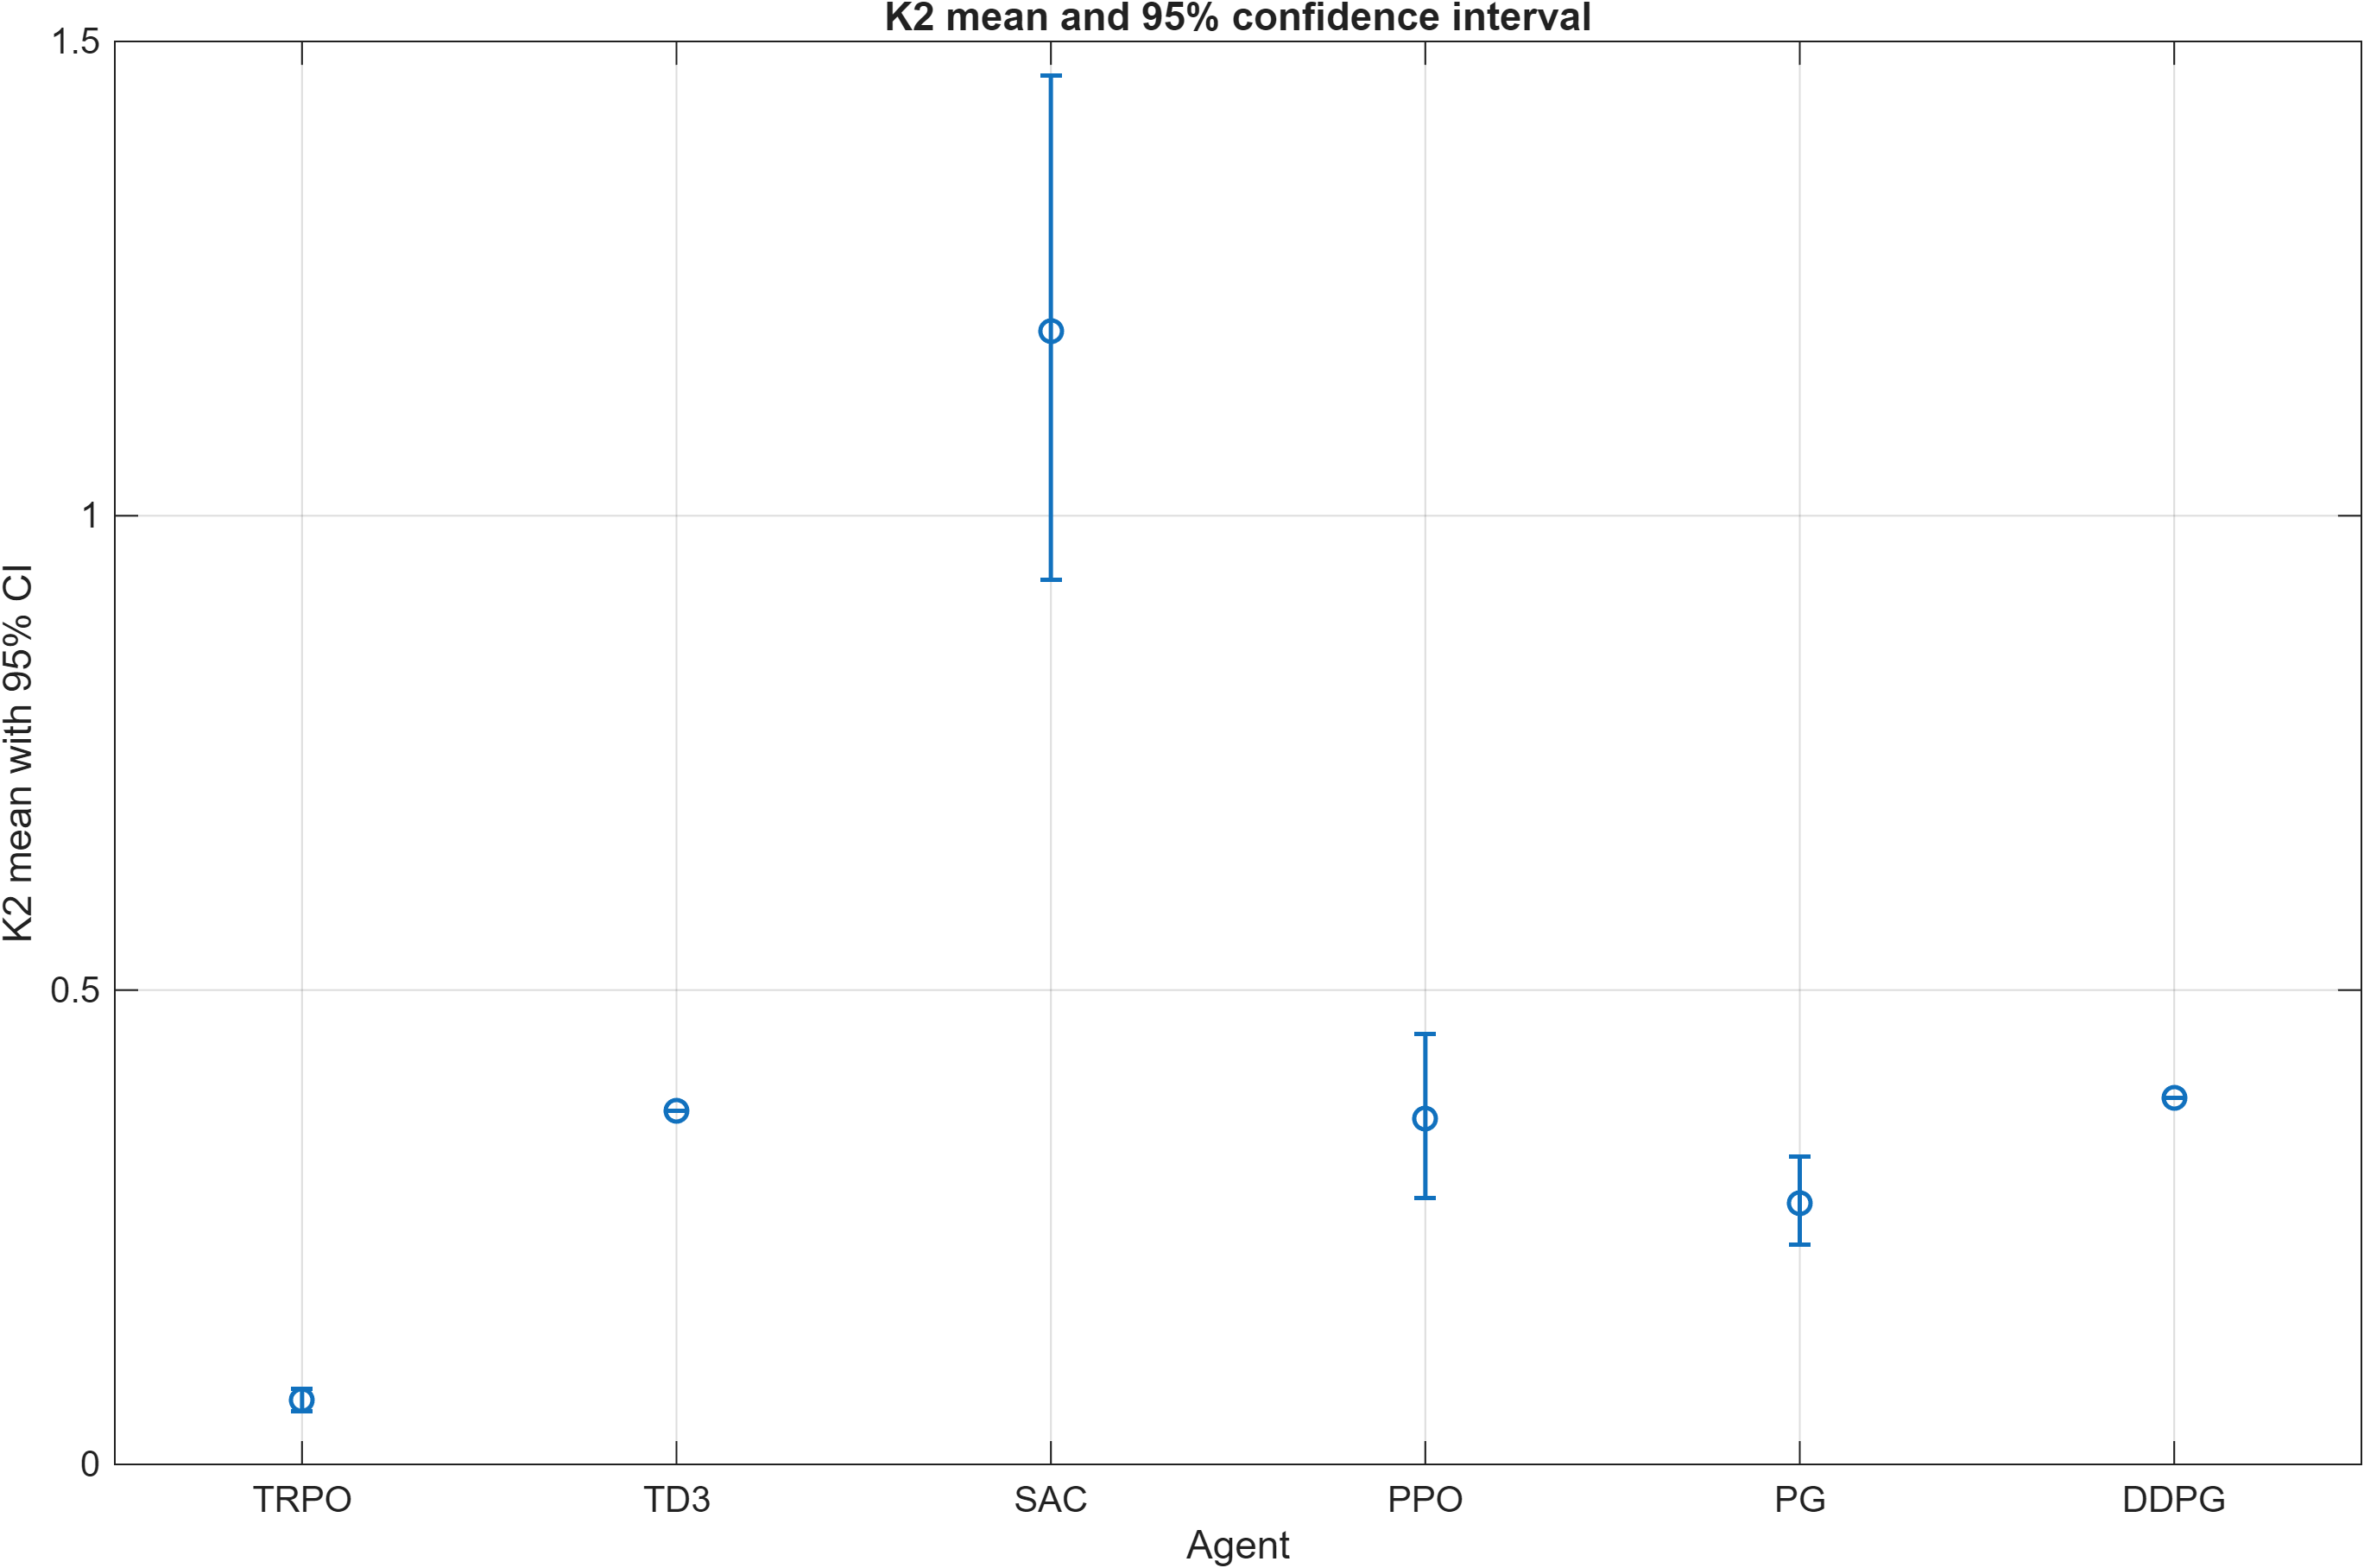
\includegraphics[width=\linewidth]{Figures/ci_K2.png}
    \caption{$K_2$: Mean Squared EE Position Error}
    \label{fig:ci_k2}
  \end{subfigure}
  \hfill
  \begin{subfigure}{0.48\textwidth}
    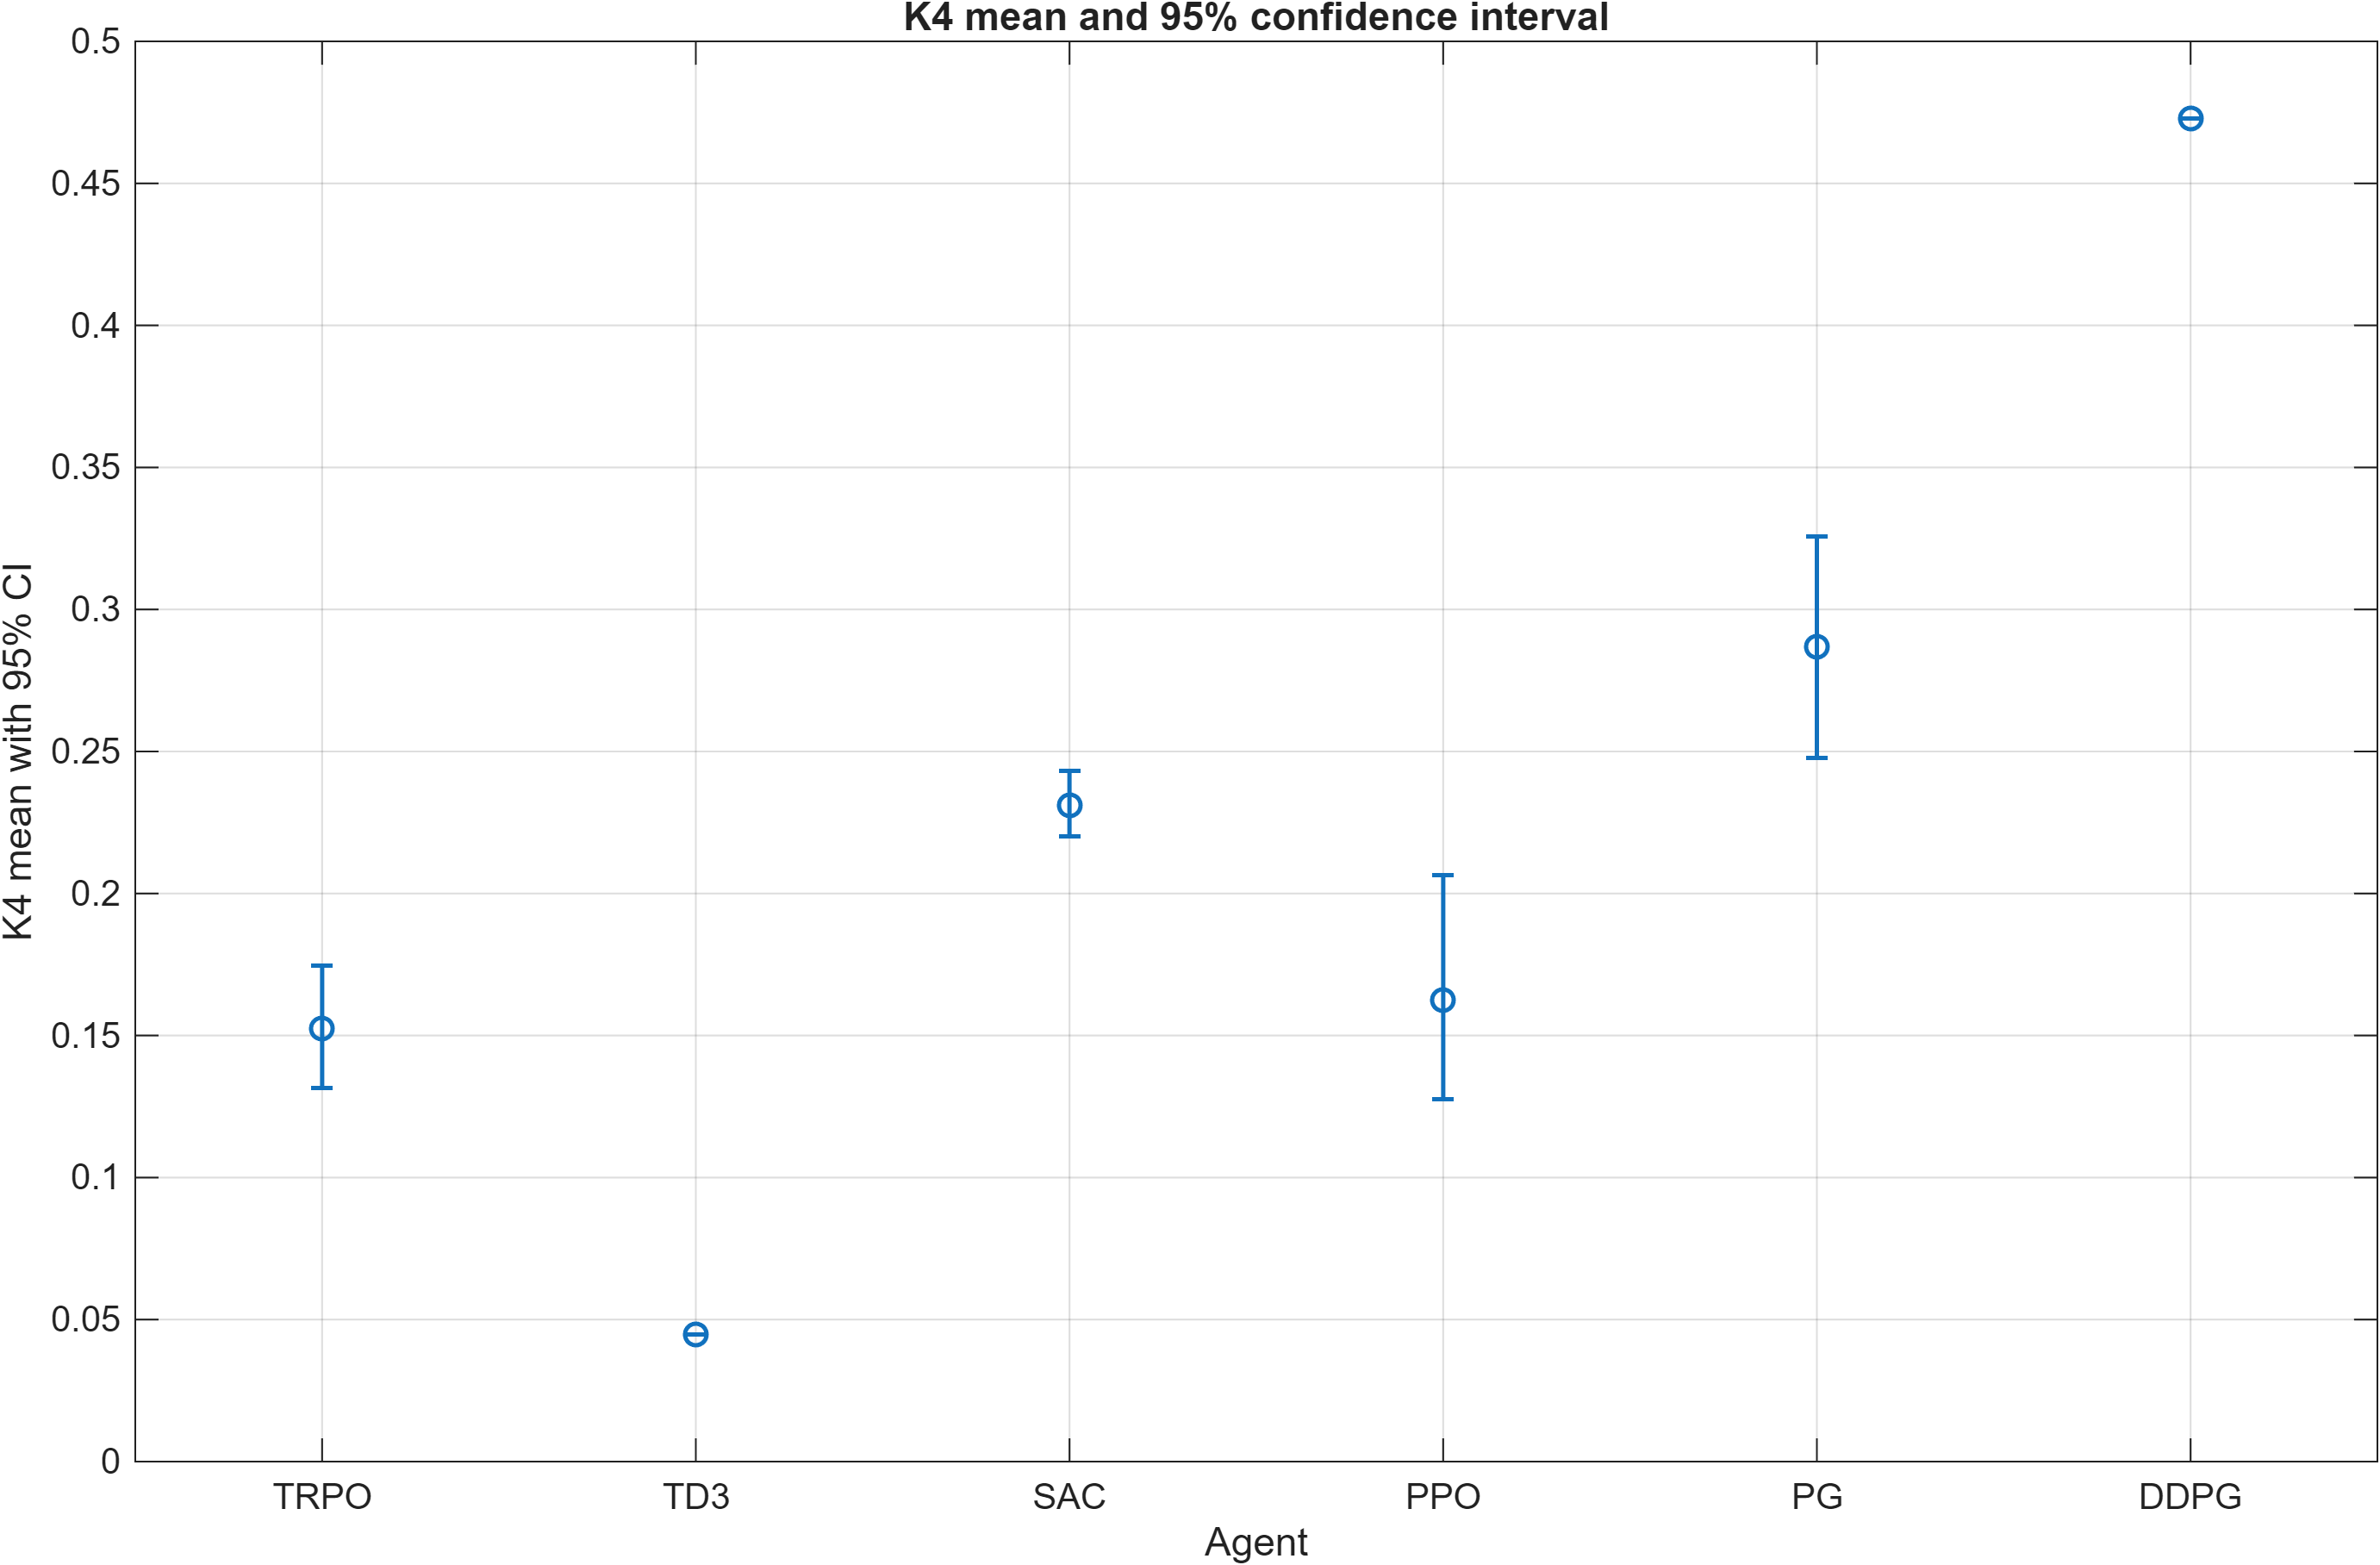
\includegraphics[width=\linewidth]{Figures/ci_K4.png}
    \caption{$K_4$: Mean Base Orientation Error}
    \label{fig:ci_k4}
  \end{subfigure}
  \\[6pt]
  \begin{subfigure}{0.48\textwidth}
    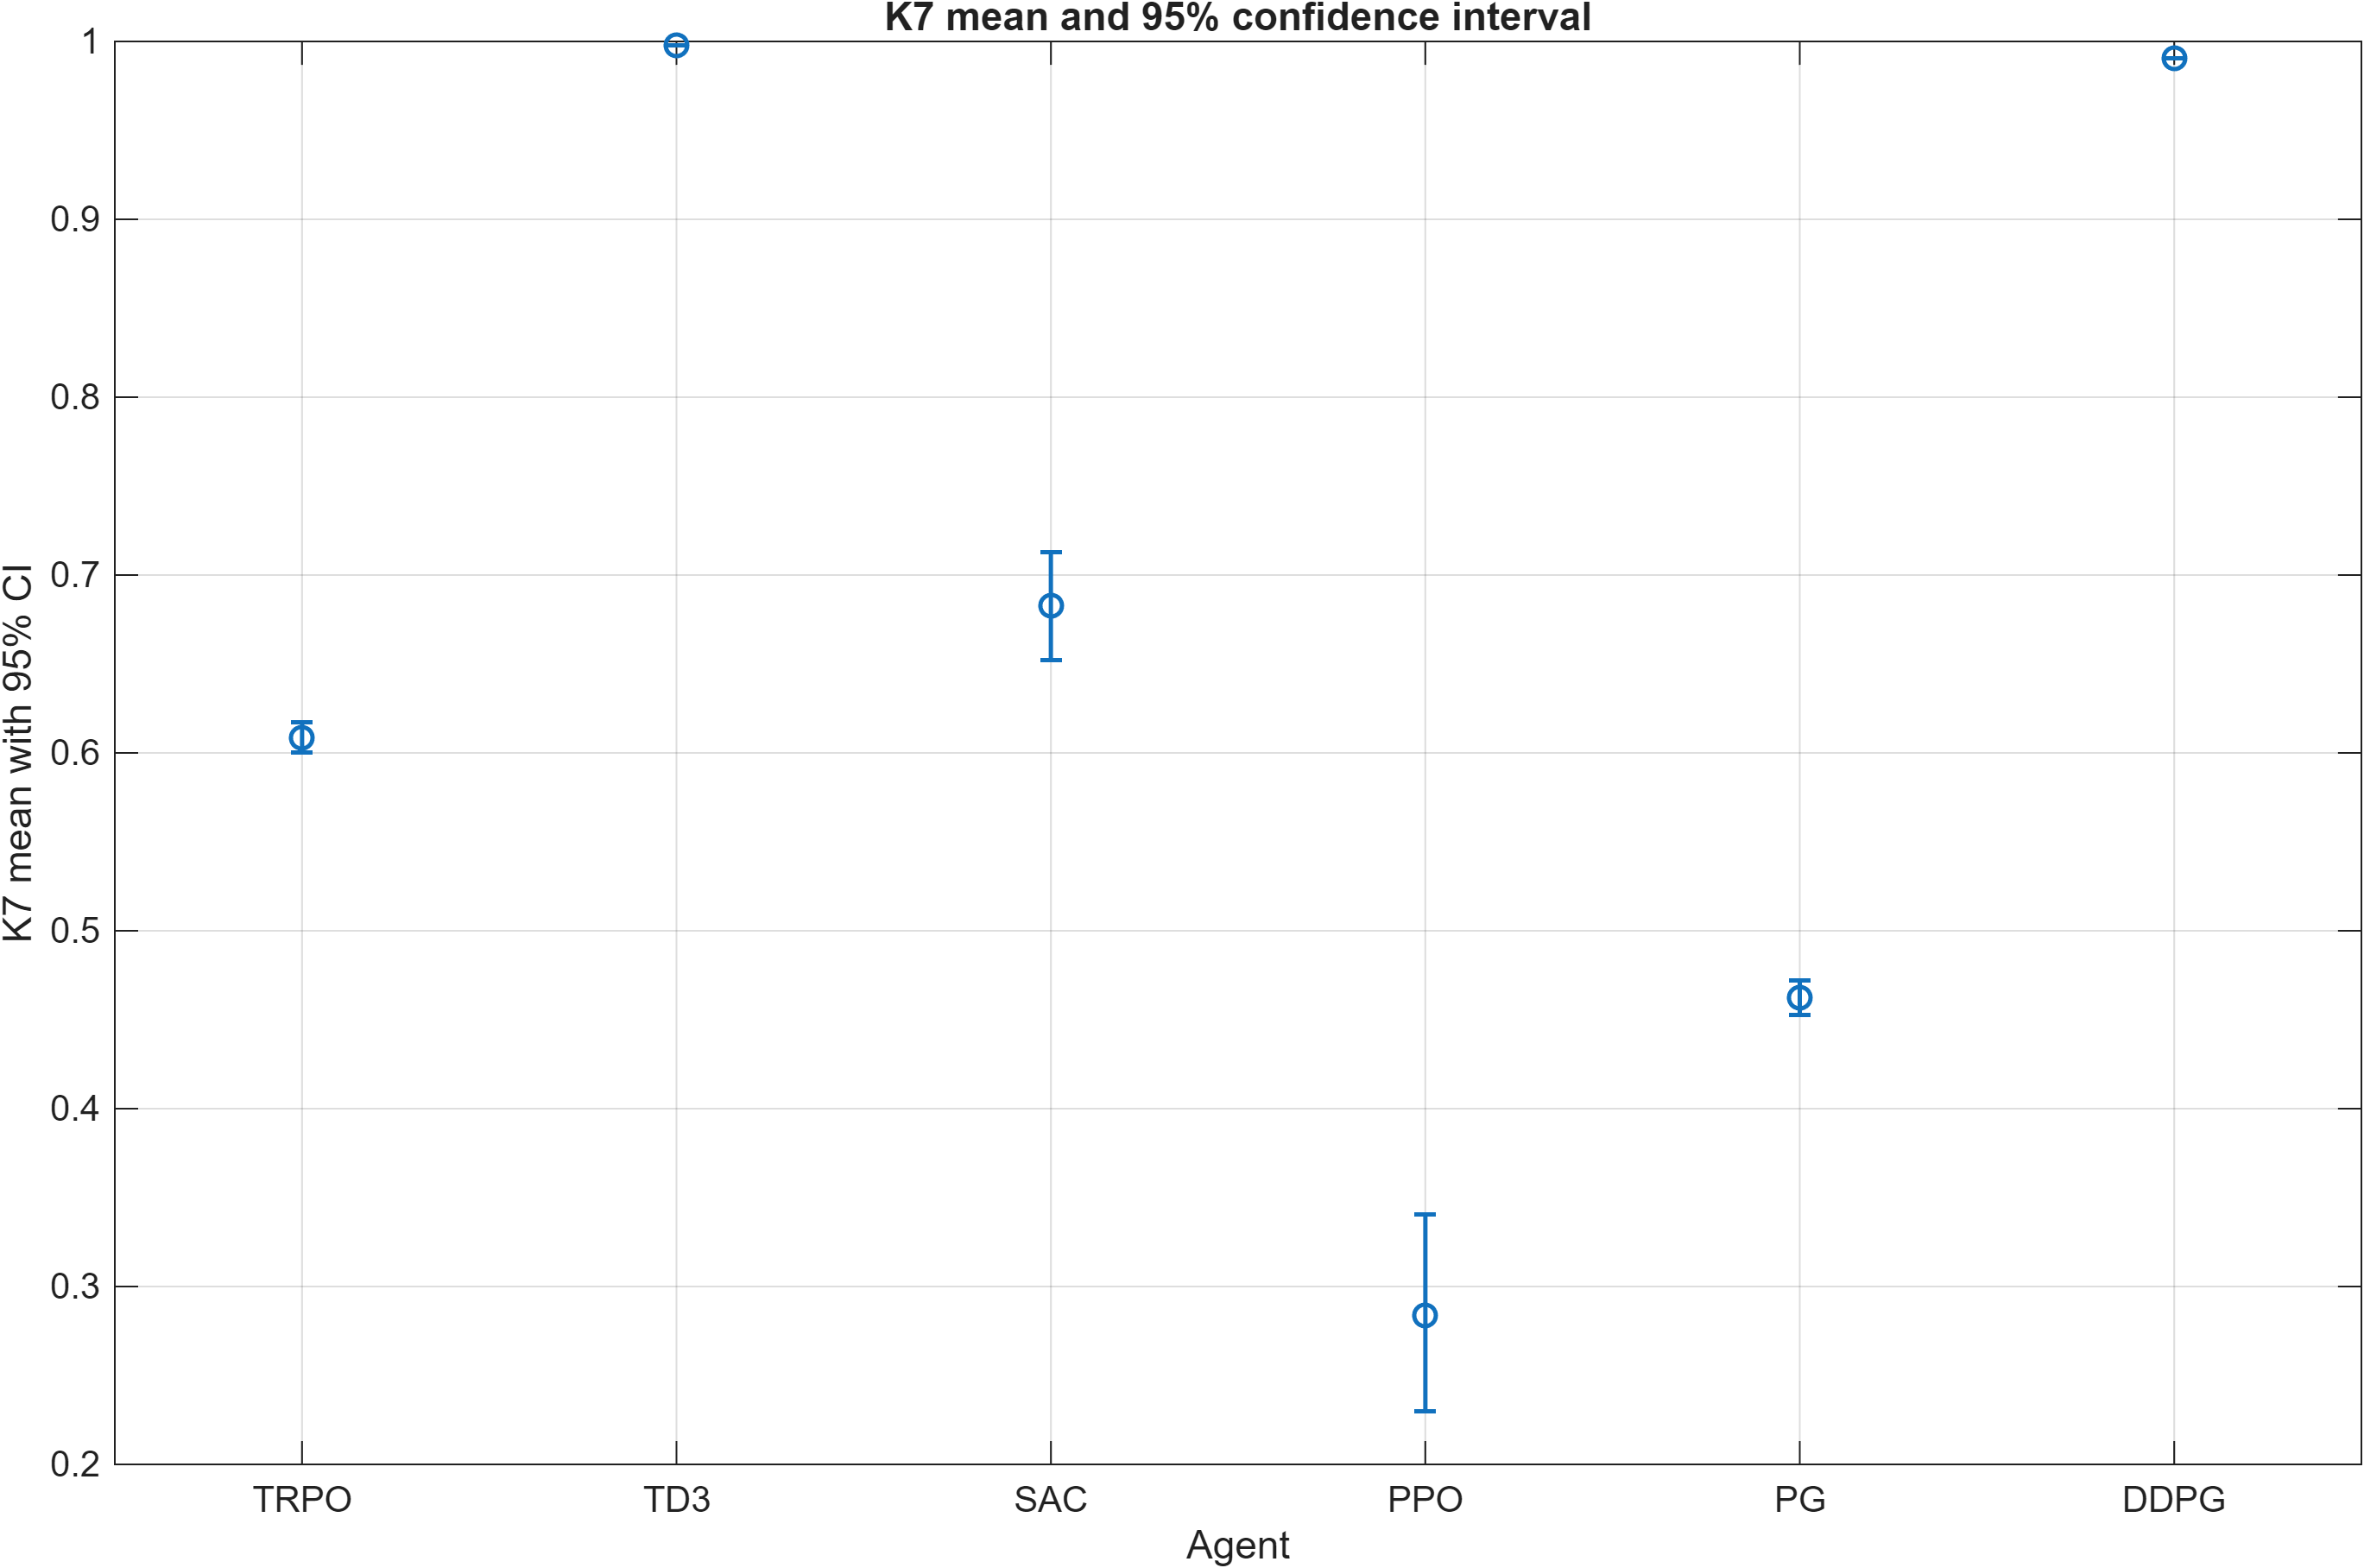
\includegraphics[width=\linewidth]{Figures/ci_K7.png}
    \caption{$K_7$: Control Smoothness (Jerk)}
    \label{fig:ci_k7}
  \end{subfigure}
  \hfill
  \begin{subfigure}{0.48\textwidth}
    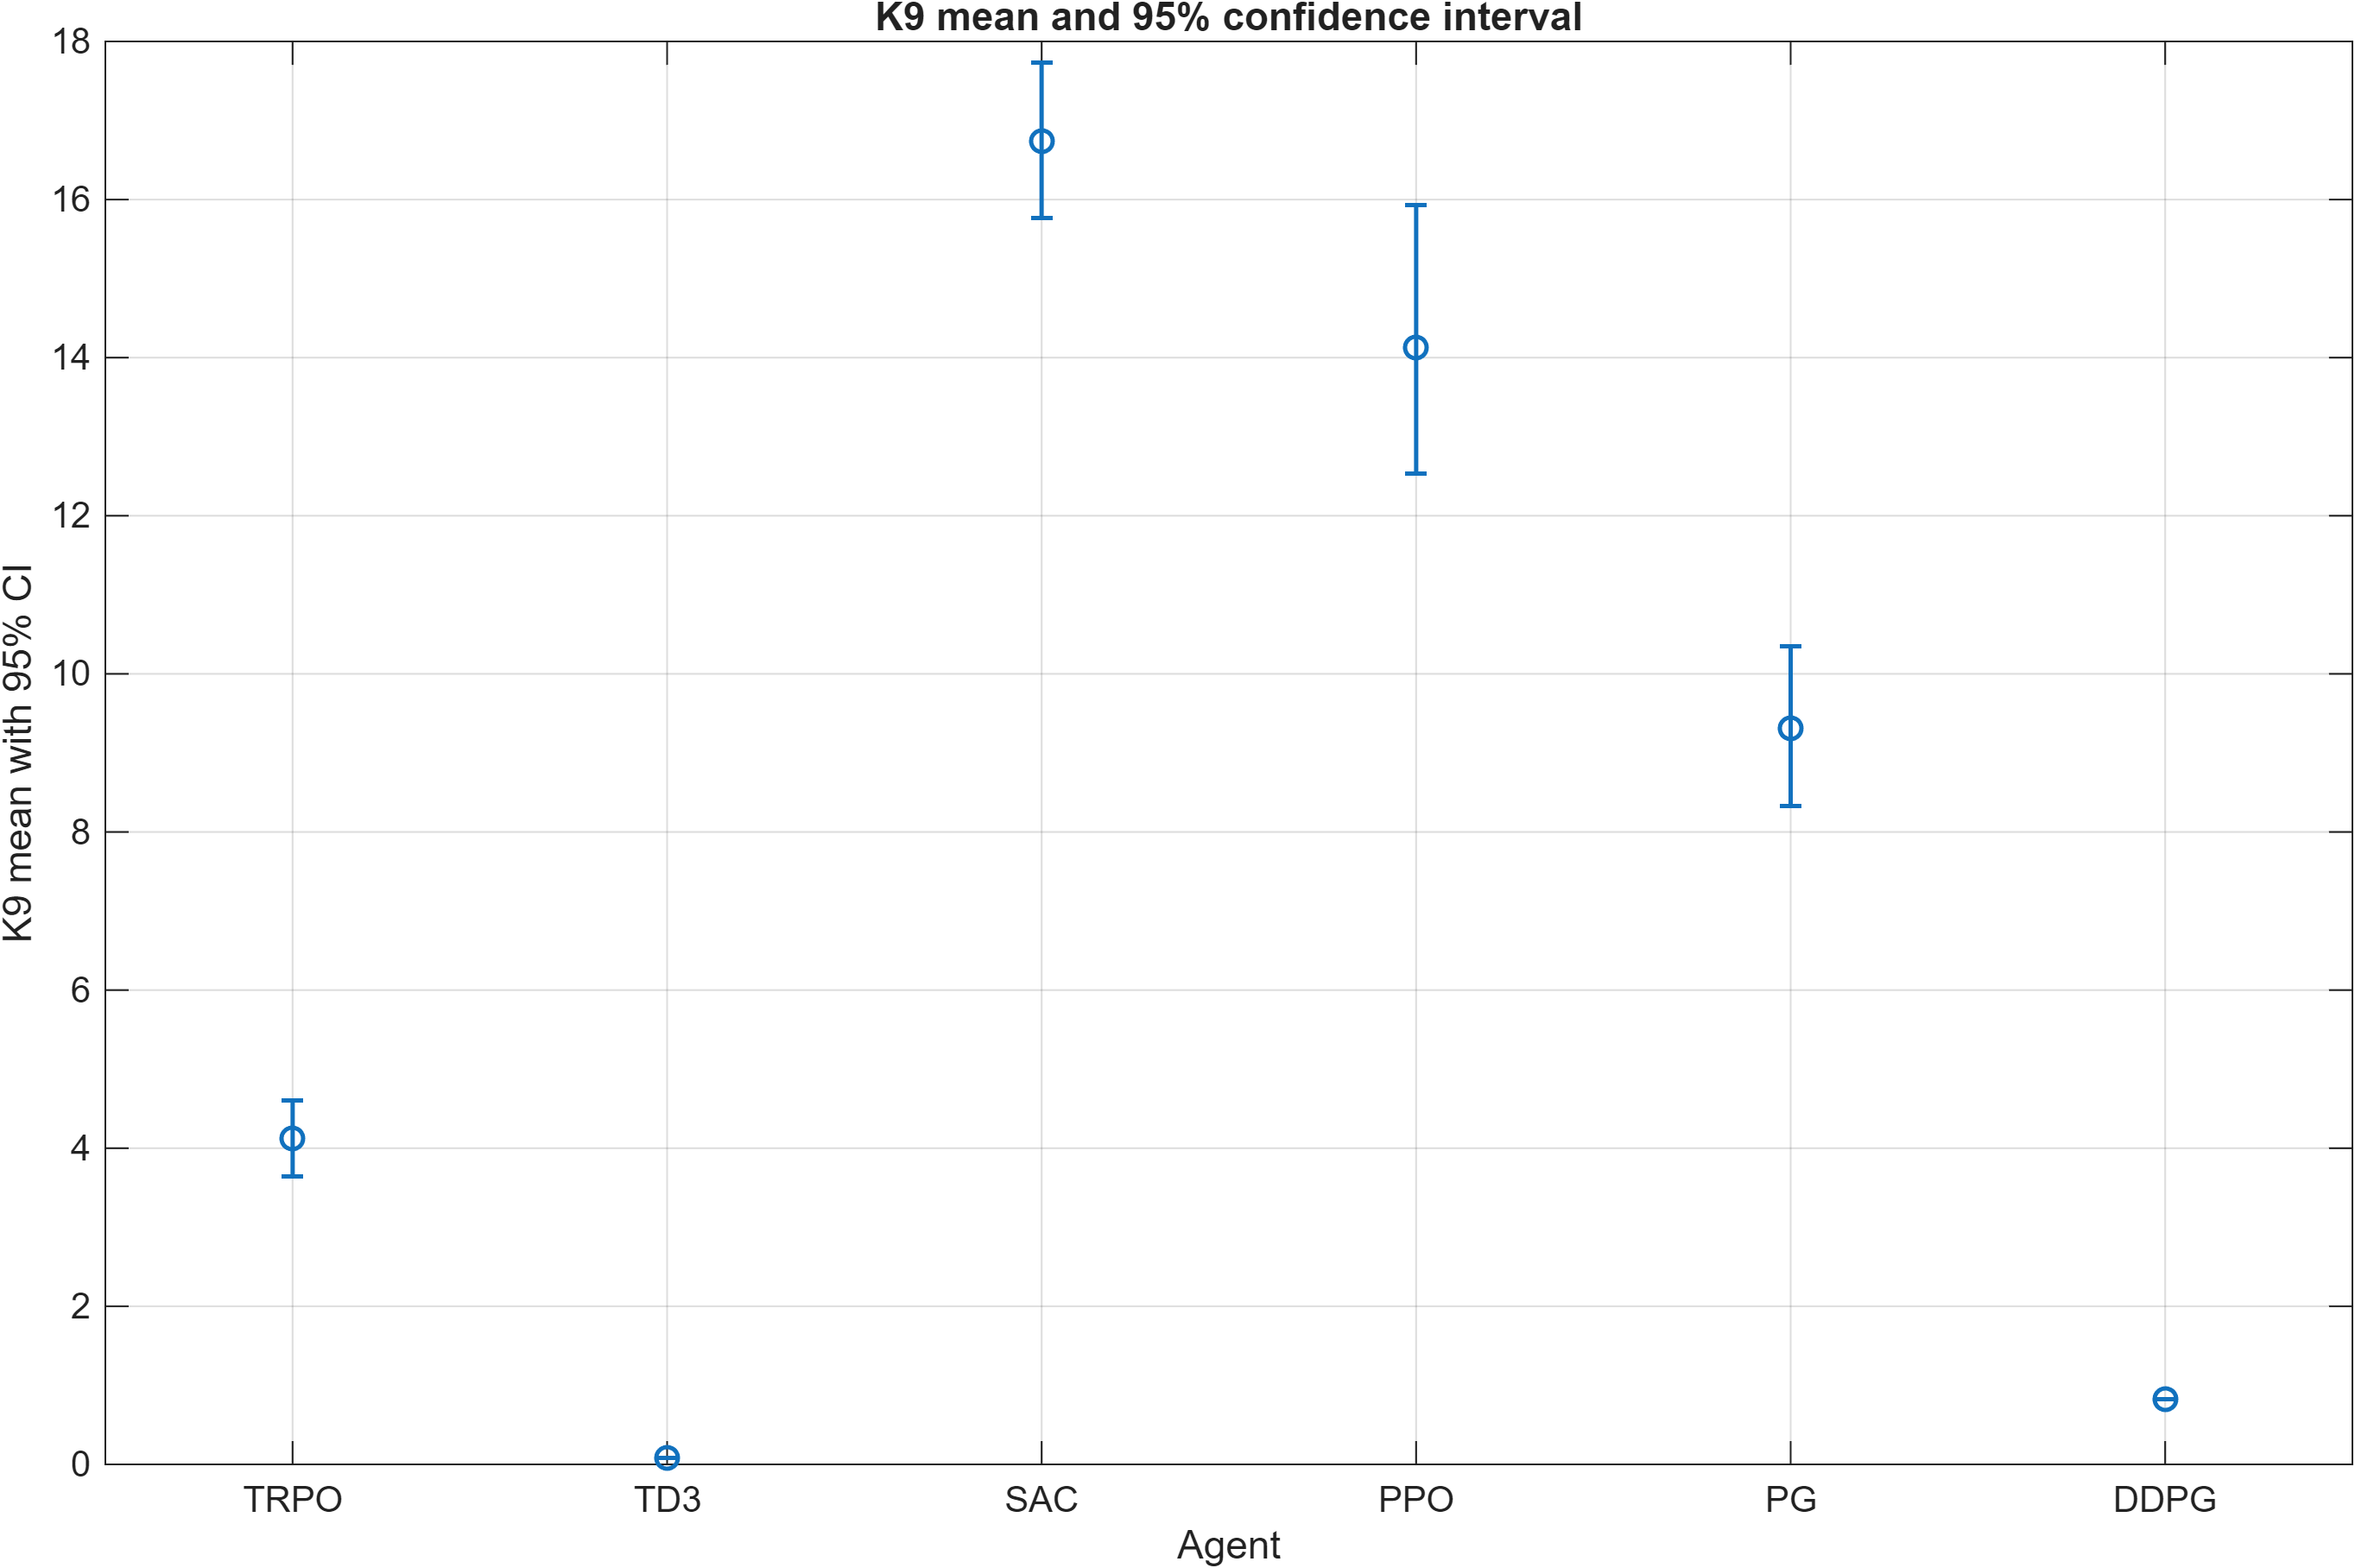
\includegraphics[width=\linewidth]{Figures/ci_K9.png}
    \caption{$K_9$: Energy Consumption}
    \label{fig:ci_k9}
  \end{subfigure}
  \caption{Mean and 95\% bootstrap confidence interval of selected KPIs over the successful runs of each
    agent (2000 resamples). The number of successful runs is given below each agent. The intervals of
    agents with few successful runs are wide or undefined. The optimized PPO agent of \cref{sec:ppo_opt}
    is included for reference.}
  \label{fig:ci_plots}
\end{figure*}

\textbf{Summary of the Comparison.} With the toolbox default hyperparameters, the comparison can be
summarized as follows:
\begin{itemize}
  \item TRPO was the only default agent that completed all ten runs without a terminated evaluation
  episode. It also reached a low tracking error, although three of its runs were weaker than the others.
  \item The default PPO agent and PG succeeded in only three and two of ten runs. Their successful runs
  tracked the path with an error similar to that of TRPO.
  \item SAC, TD3, and DDPG succeeded in four to six runs. Even in their successful runs, they showed
  significantly larger tracking errors than TRPO and required two to three times longer training.
\end{itemize}
These results suggest that the trust-region constraint of TRPO stabilizes training under the strong
base--manipulator coupling. The clipped updates of PPO did not provide the same stability with the
default learning rate of $10^{-2}$. This learning rate is high for PPO and the off-policy methods and
likely contributes to their seed dependence. PPO is selected for tuning in \cref{sec:ppo_opt} because
its successful runs were competitive with TRPO and it trained faster than TRPO. The tuning therefore
targets the seed dependence.

\section{Optimization of the PPO Agent}\label{sec:ppo_opt} The default PPO agent succeeded
in only three of ten runs in \cref{comparison}, but its successful runs tracked the path with an
error similar to that of TRPO. This section examines whether a tuned configuration removes this seed
dependence. The PPO agent used so far corresponds to the default configuration of MATLAB's Reinforcement
Learning Toolbox \cite{b4}. The tuning concerns the hyperparameters and the output layer of the policy
mean, while the hidden layers of the networks are kept.



\begin{figure*}[!t]
	\centering
	\begin{subfigure}{0.48\textwidth}
		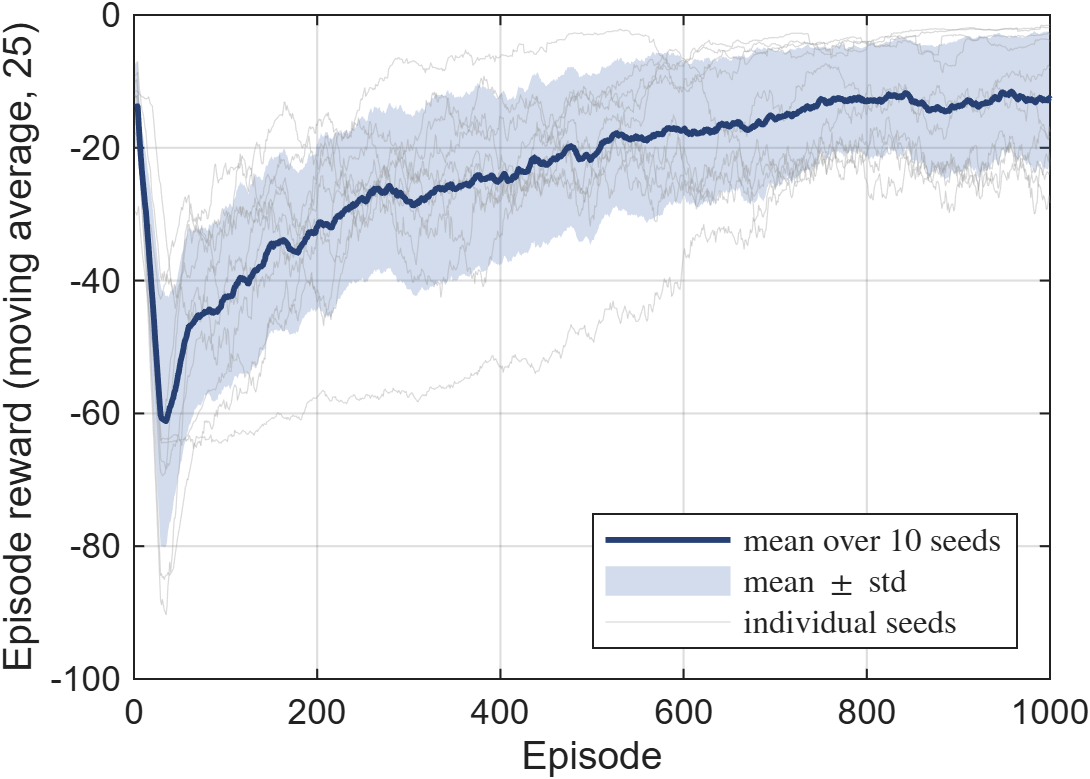
\includegraphics[width=\linewidth,height=0.25\textheight]{Figures/trainingsverlauf_ppo_default.png}
		\caption{PPO (default)}
		\label{fig:training_ppo_default}
	\end{subfigure}
	\hfill
	\begin{subfigure}{0.48\textwidth}
		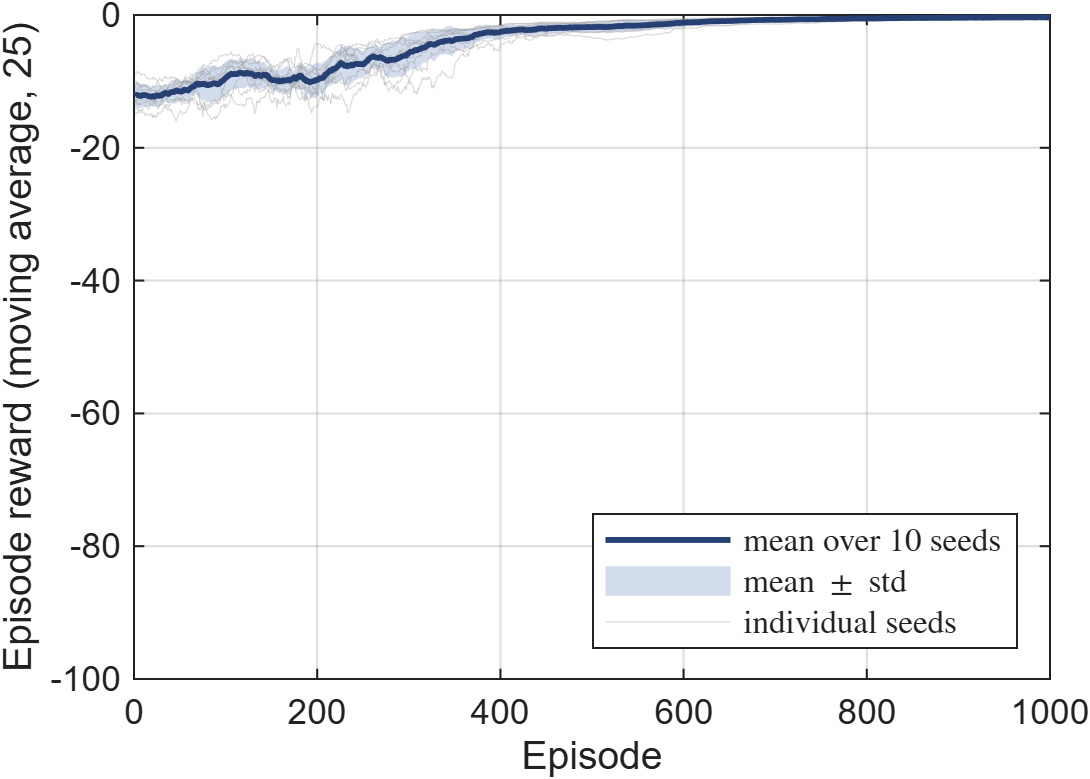
\includegraphics[width=\linewidth, height=0.25\textheight]{Figures/trainingsverlauf_ppo_optimized.png}
		\caption{PPO (optimized)}
		\label{fig:training_ppo_opt}
	\end{subfigure}
	\caption{Episode rewards during training of the default and the optimized PPO agents over ten seeds. The
  thin lines show the moving average over 25 episodes of each seed, the thick line the mean over the seeds,
  and the band one standard deviation. Both panels use the same axis. (a) Default hyperparameters.
  (b) Optimized configuration.}
	\label{fig:training_ppo_compare}
\end{figure*}
\textbf{Network Architecture.} The optimized agent keeps the hidden layers of the default PPO agent. The
policy and the value network both use two hidden layers of 128 units with ReLU activations. In contrast
to the default agent, the mean output of the Gaussian policy is not bounded by a tanh layer.
The commanded torques are limited by the saturation block instead. The networks are defined explicitly
rather than through the toolbox default constructor.

\textbf{Hyperparameter Tuning.} The configuration was determined in a preliminary
coordinate-wise grid search and is kept fixed for all experiments reported here. The search
used a single training run per candidate. It was carried out on an earlier version of the simulation
model, before the reward weights, the termination rule, and the evaluation protocol of this work were
fixed. The selected values are therefore used as a fixed configuration and are not claimed to be optimal
for the final setup. Each hyperparameter was swept over a discrete set of candidate values while all
others were held at their current best values. The configuration with the highest mean episodic reward
over the final 50 of the $N_{\mathrm{train}}=1000$ training episodes was selected. In total, 16 training
runs of 1000 episodes each were conducted during this tuning phase. The swept parameters, their candidate
values, and the selected values are as follows:
\begin{itemize}
  \item \textit{Actor learning rate.} Candidates $\{1\!\times\!10^{-3},\;5\!\times\!10^{-4}\}$,
  selected $1\!\times\!10^{-3}$. Both candidates are an order of magnitude below the toolbox
  default of $10^{-2}$, which reduces the size of the policy updates.
  \item \textit{Critic learning rate.} Candidates $\{1\!\times\!10^{-3},\;5\!\times\!10^{-4}\}$,
  selected $5\!\times\!10^{-4}$, which gave the highest mean episodic reward in the search.
  \item \textit{Entropy loss weight.} Candidates $\{1\!\times\!10^{-2},\;1\!\times\!10^{-3}\}$, selected
  $1\!\times\!10^{-3}$. A small entropy bonus is intended to prevent a premature convergence to a
  suboptimal deterministic policy while avoiding undirected exploration.
  \item \textit{Experience horizon.} Candidates $\{512,\;1024,\;2048\}$, selected $1024$. A moderate rollout horizon
  is a compromise between the trajectory information per update and the memory requirements and update latency.
  \item \textit{Mini-batch size.} Candidates $\{128,\;256\}$, selected $256$. Larger mini-batches are expected to give
  more stable gradient estimates and thus a lower training variance.
  \item  \textit{Fixed settings.} The discount factor was set to $\gamma = 0.995$,
  the number of epochs per update to 10, and the gradient threshold of both optimizers to 1. The
  clip factor of 0.2 and the GAE factor of 0.95 remain at their default values.
\end{itemize}

In the tuning runs, the selected configuration gave the highest mean episodic reward. Compared with the
default configuration, the optimized agent uses learning rates that are ten to twenty times smaller,
larger rollouts and mini-batches, more epochs per update, and gradient clipping. Together, these settings
limit the size of each policy update. In addition, its policy mean has no tanh output layer. The
comparison with the default PPO agent therefore reflects both changes, and their individual effects
were not separated.

\subsection{Circular Trajectory}

\textbf{Training Outcome.} \cref{fig:training_ppo_compare} shows the training curves of both
configurations over ten seeds. The moving-average return of the default PPO agent dropped to about $-61$
within the first 35 episodes and then rose slowly to $-12.7$ after 1000 episodes, with a large spread
between the seeds. The optimized configuration started at about $-12$, exceeded $-1$ after 625 episodes,
and reached $-0.36$ with a small spread between the seeds. For comparison, TRPO reached $-0.81$ after 1000
episodes.

\textbf{Success and Performance.} \cref{tab:ppo_optimization_kpi} compares the optimized PPO agent with the
default PPO agent and with TRPO. The optimized configuration completed all ten runs without a terminated
evaluation episode, compared with three runs for the default configuration (Fisher's exact test,
$p = 0.003$). Over the successful runs, it reached a mean squared tracking error of $K_2 = 0.0041$,
compared with 0.0134 for the default PPO agent and 0.0145 for TRPO. The base orientation error $K_4$ was
0.021, compared with 0.050 and 0.026. The optimized agent also produced smoother torque commands than the
default PPO agent ($K_7$, $0.383 \to 0.0097$) with a lower energy consumption ($K_9$, $12.4 \to 2.16$).
Its control smoothness and energy consumption were similar to those of TRPO.

\textbf{Comparison With TRPO.} On the seed level, only the difference in the base orientation error
$K_4$ had an uncorrected $p$-value below 0.05 (Mann--Whitney, $p = 0.045$). The differences in the
return $K_1$, the tracking error $K_2$, and the base angular velocity $K_8$ had $p$-values between 0.076
and 0.089. After a Holm correction over the seven tested KPIs, none of the differences was significant.
The optimized agent trained in 9.2\,min per run, compared with 11.3\,min for TRPO.

\begin{figure*}[t]
    \centering
    \begin{subfigure}{0.48\textwidth}
        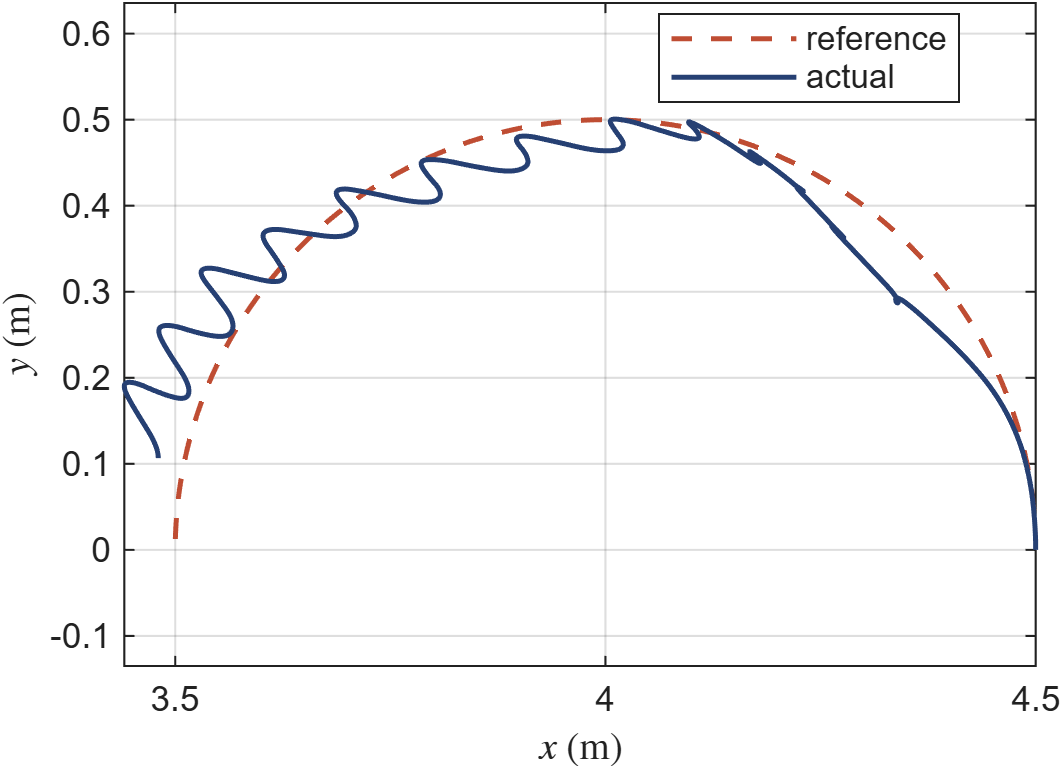
\includegraphics[width=\linewidth]{Figures/soll_vs_ist_kreisbahn.png}
        \caption{PPO (default)}
        \label{fig:traj_default}
    \end{subfigure}
    \hfill
    \begin{subfigure}{0.48\textwidth}
        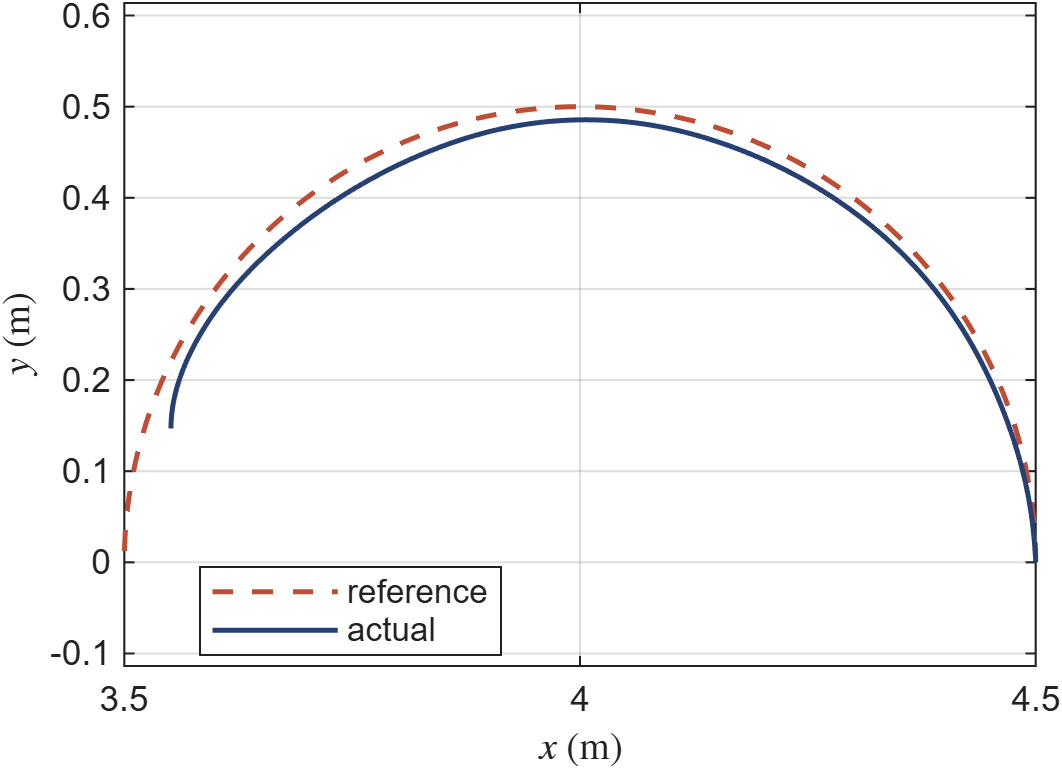
\includegraphics[width=\linewidth]{Figures/soll_vs_ist_kreisbahn_opt.png}
        \caption{PPO (optimized)}
        \label{fig:traj_opt}
    \end{subfigure}
    \caption{Reference and actual end-effector path in the $XY$ plane for one evaluation episode from the
    nominal initial state. Each panel shows the successful run with the median $K_2$ of its configuration,
    seed 2 for the default and seed 0 for the optimized PPO agent.}
    \label{fig:trajektorie_xy_compare}
\end{figure*}

\begin{figure*}[t]
    \centering
    \begin{subfigure}{0.48\textwidth}
        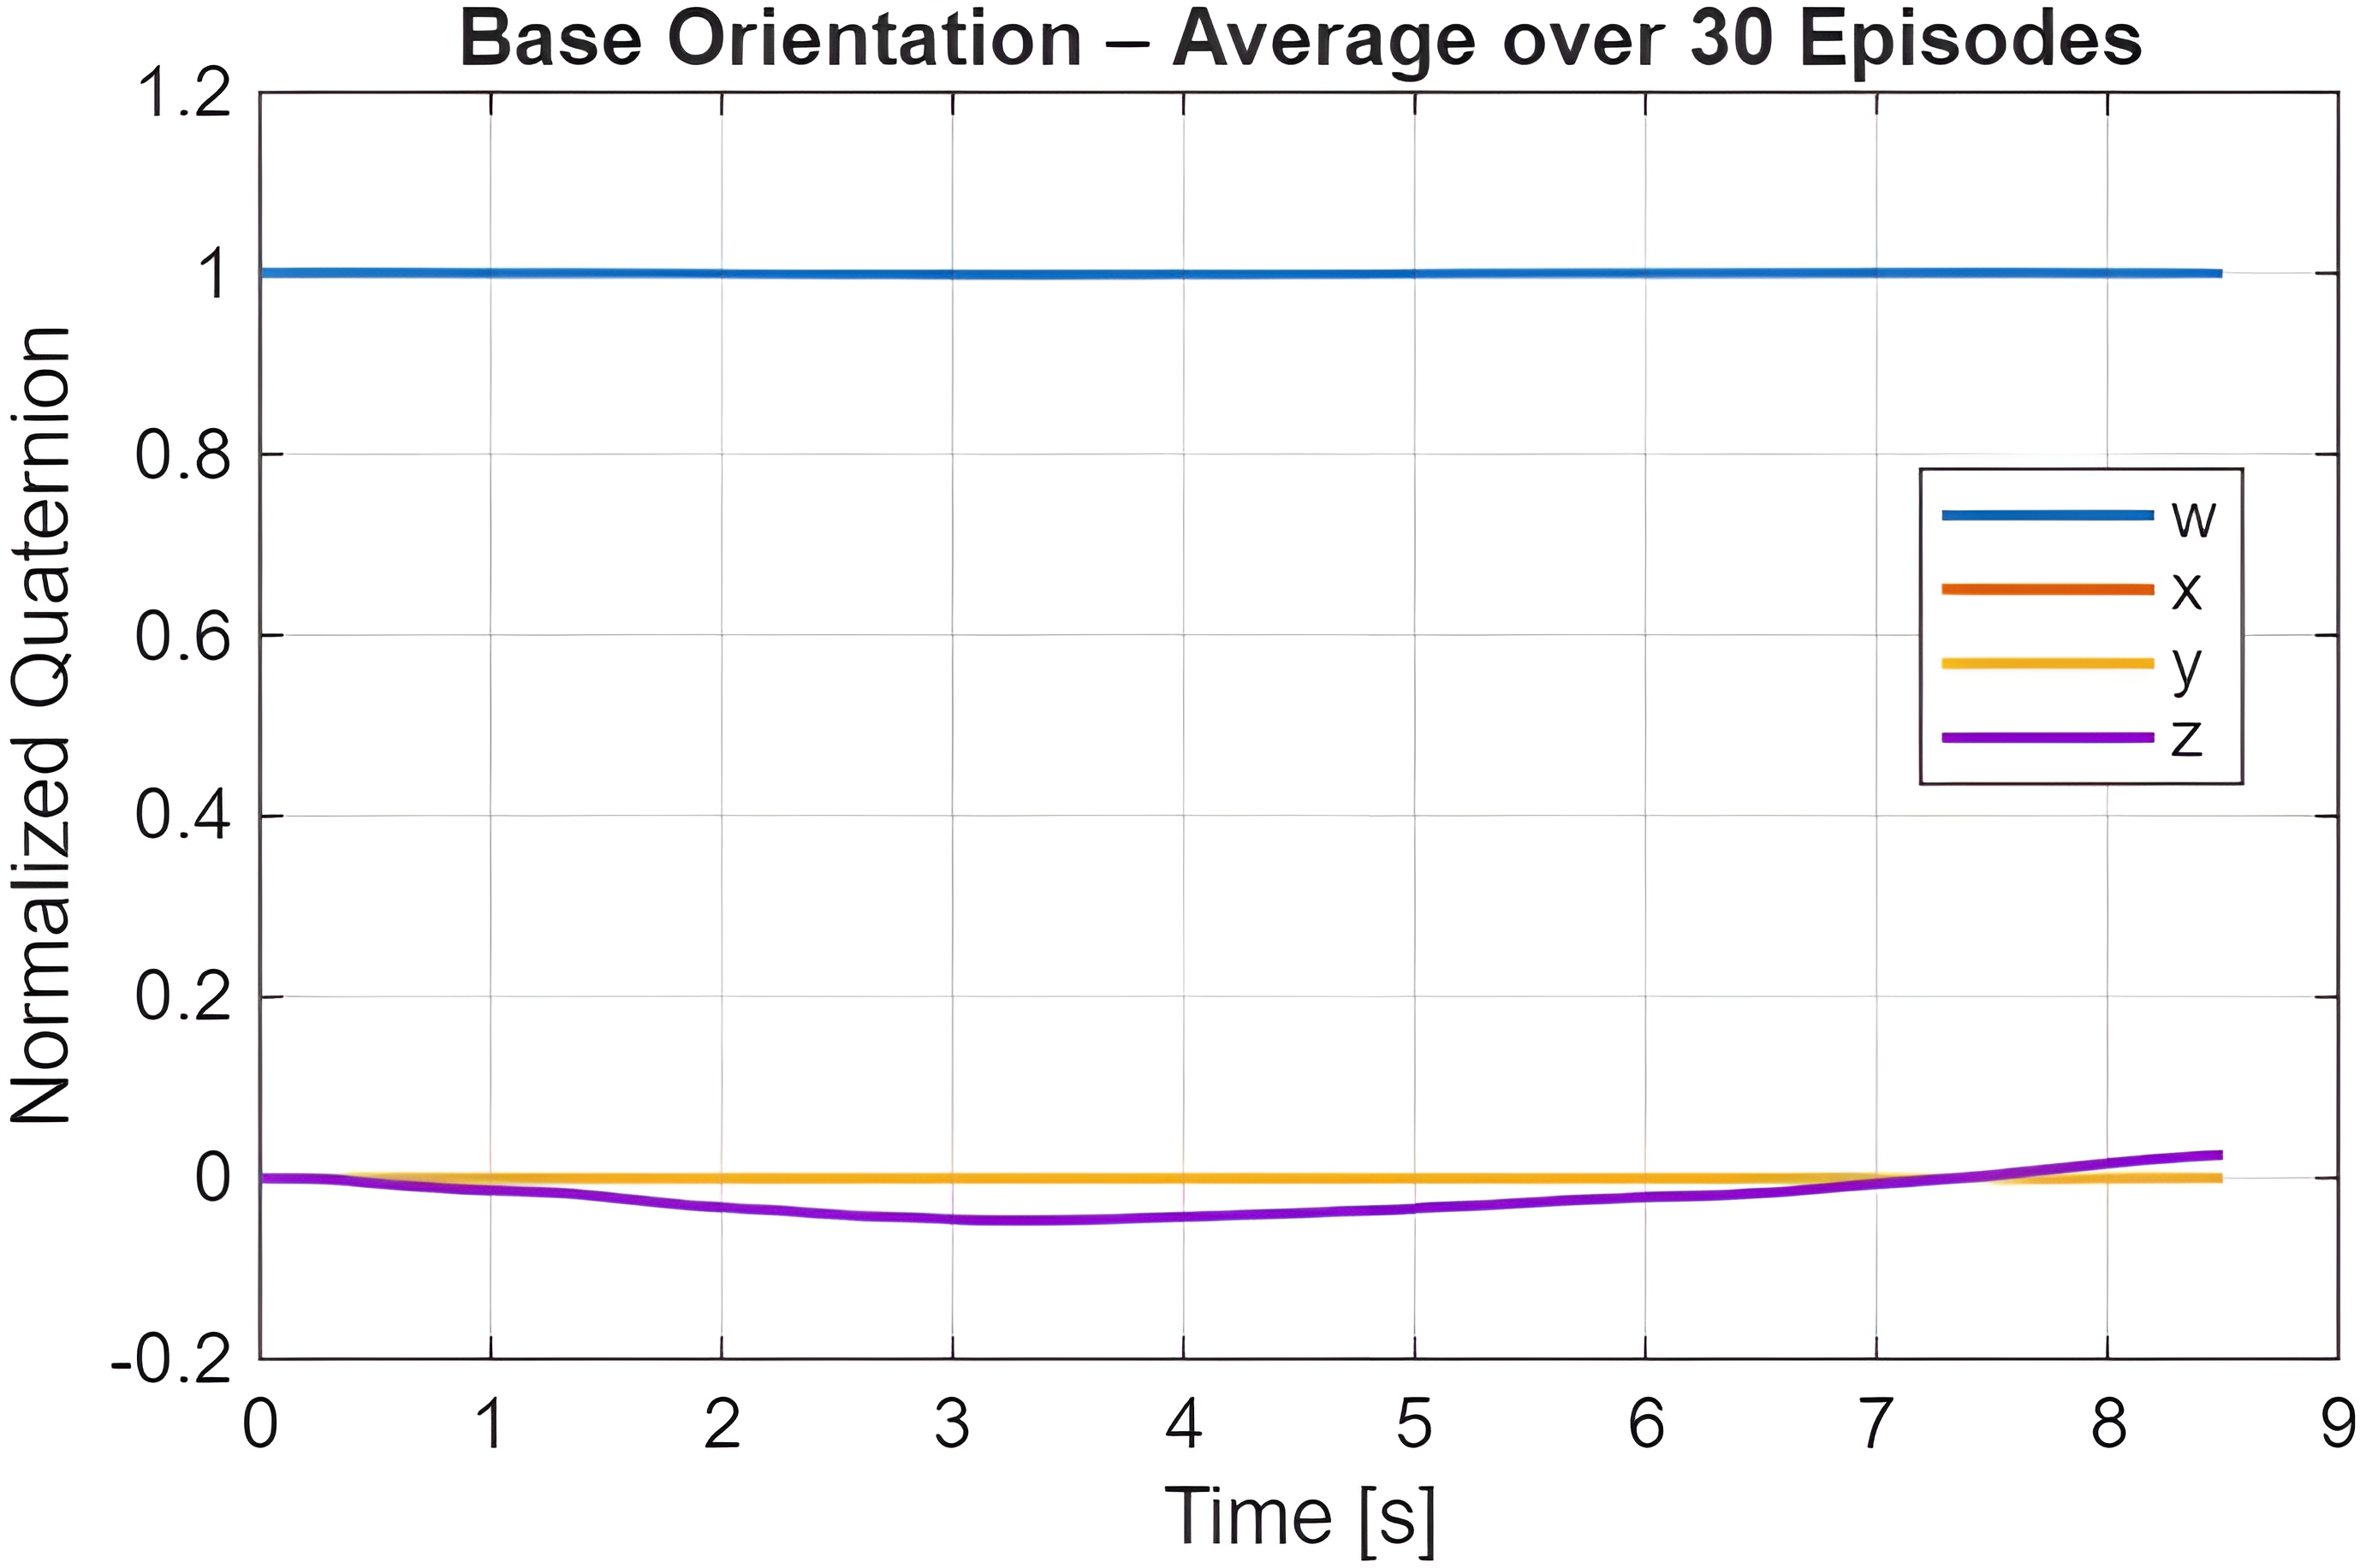
\includegraphics[width=\linewidth]{Figures/basis_orientaion_ppo.png}
        \caption{PPO (default)}
        \label{fig:basis_default}
    \end{subfigure}
    \hfill
    \begin{subfigure}{0.48\textwidth}
        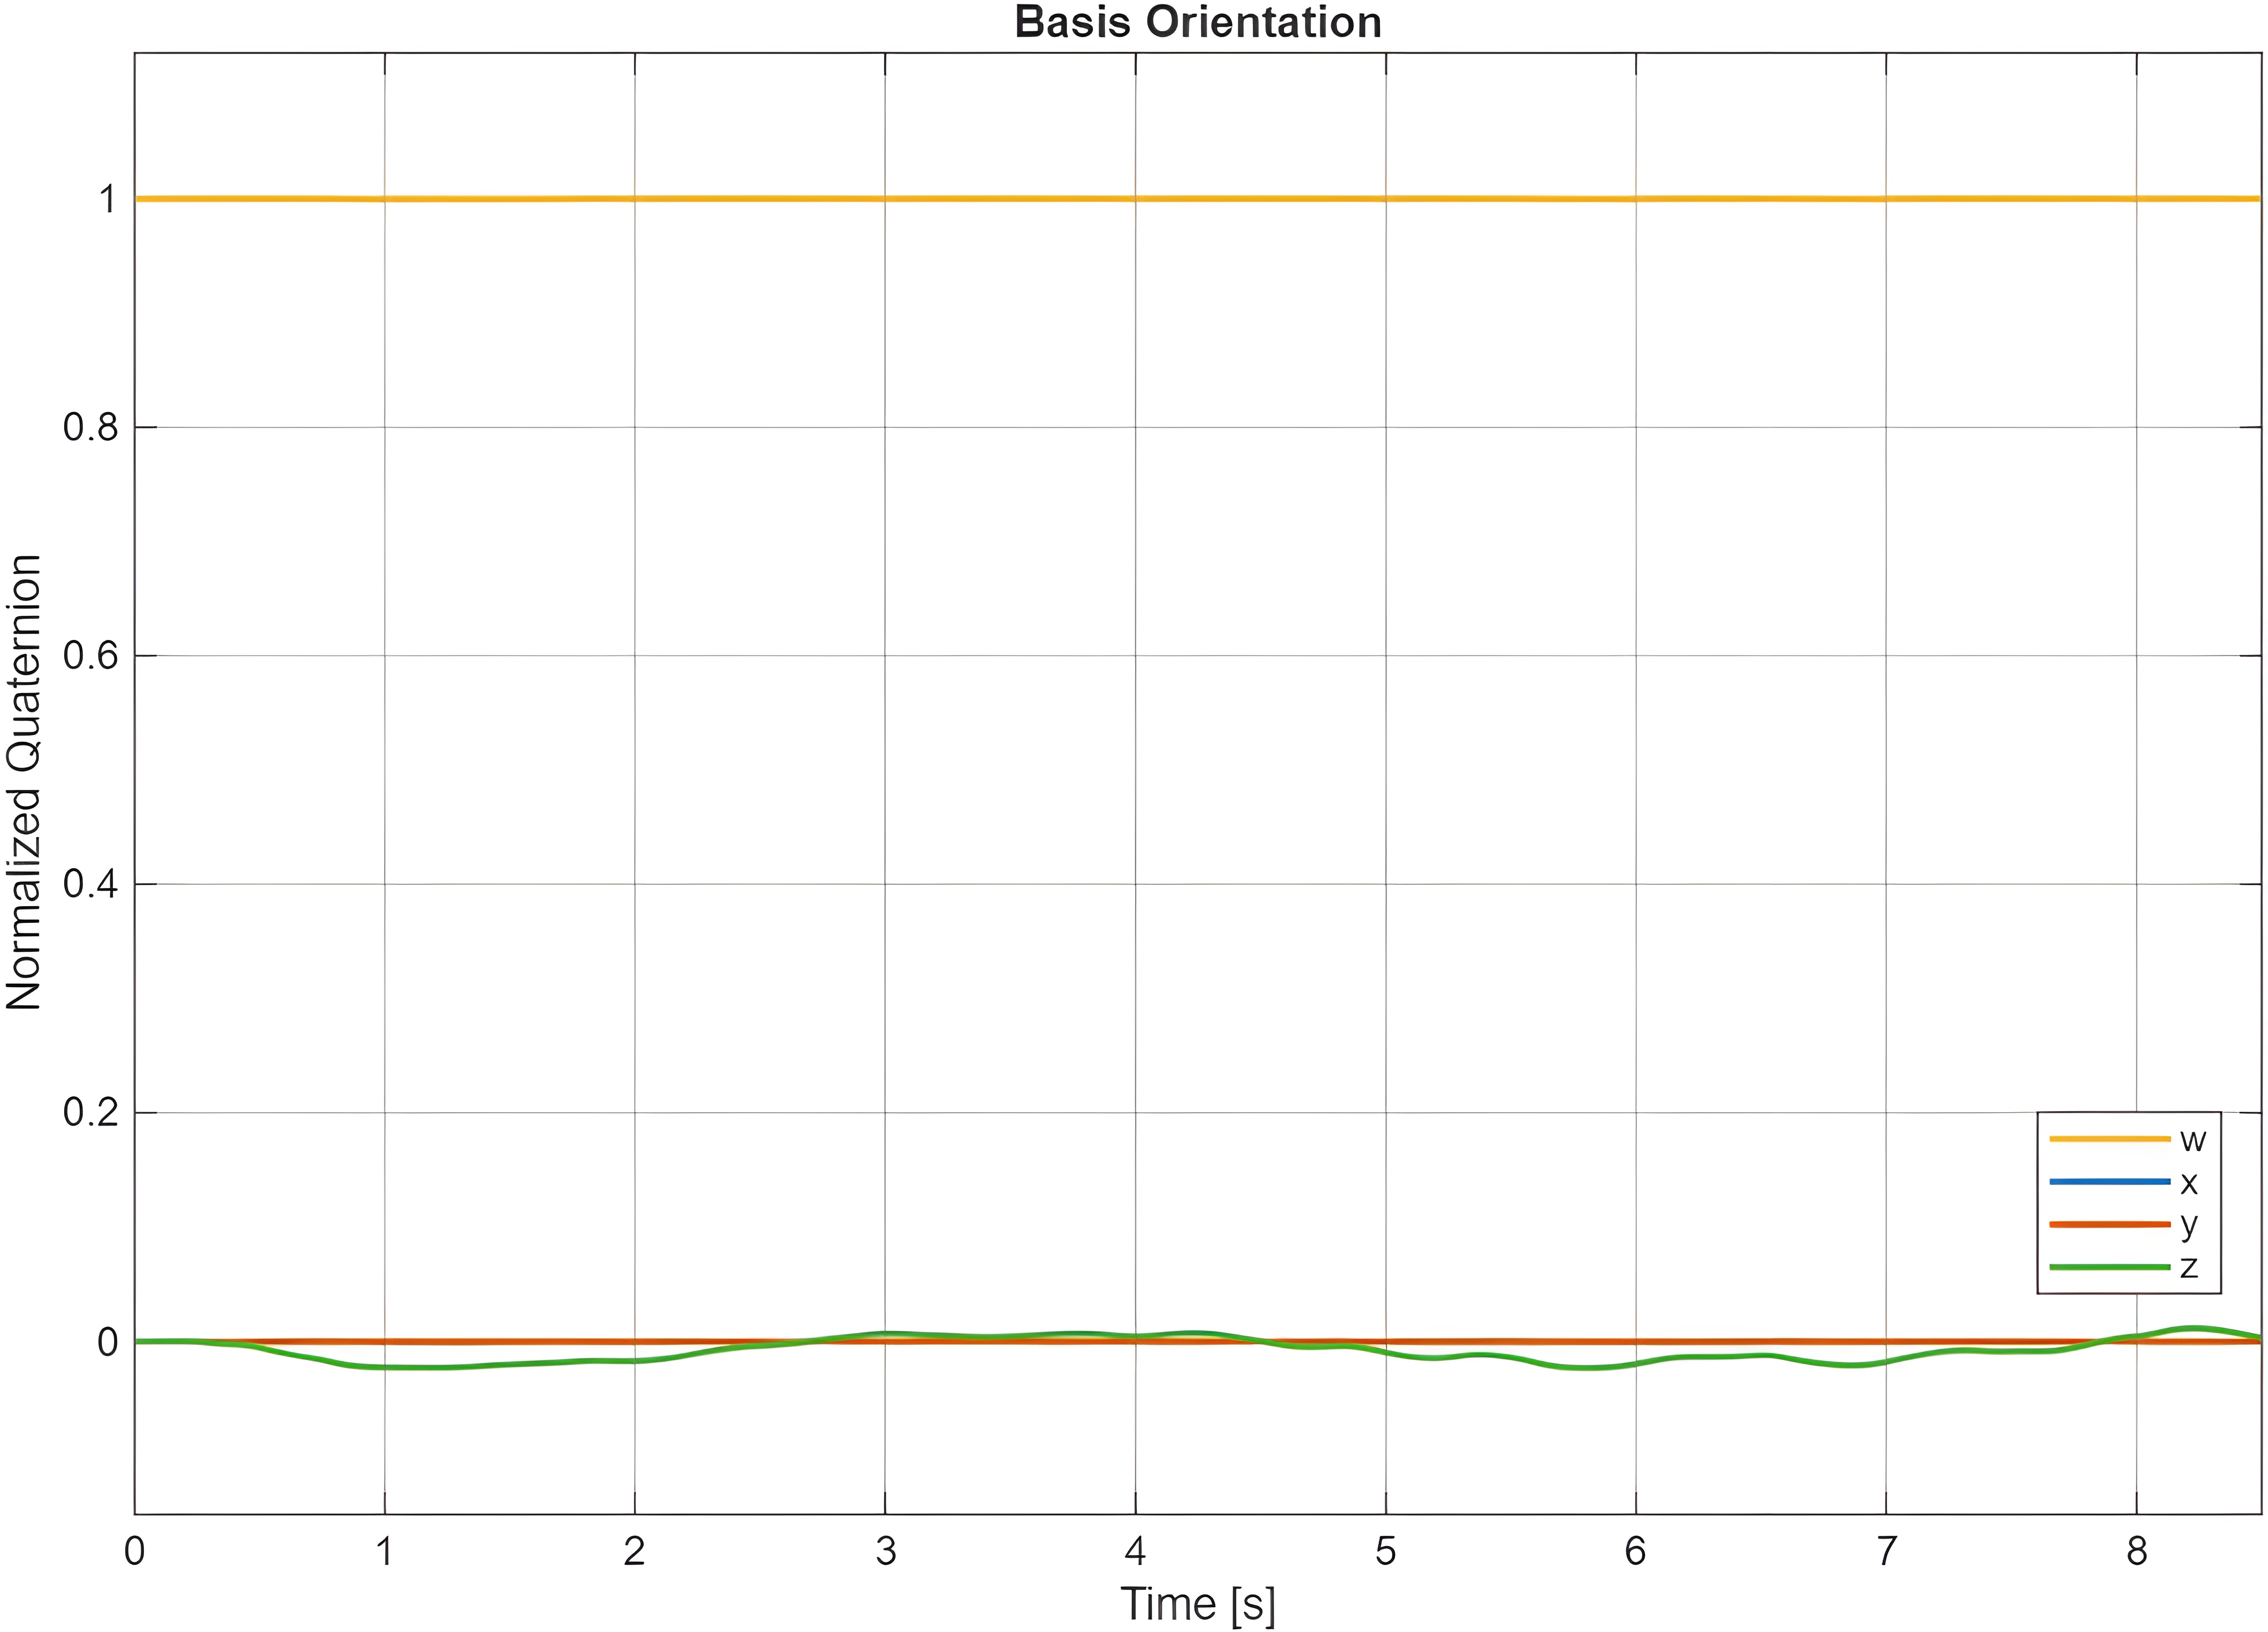
\includegraphics[width=\linewidth]{Figures/basis_orientation_ppo_optimized.png}
        \caption{PPO (optimized)}
        \label{fig:basis_opt}
    \end{subfigure}
    \caption{Vector part of the base orientation quaternion during the episodes of
    \cref{fig:trajektorie_xy_compare}. The base rotates only about the $z$-axis. The scalar part stays
    above 0.9996 in both episodes.}
    \label{fig:basis_orientation_compare}
\end{figure*}

\begin{table*}[t]
	\centering
	\caption{Default PPO agent, optimized PPO agent, and TRPO on the circular path. The first row gives the
		number of successful runs out of ten. All other values are the mean and the standard deviation over
		the successful runs. $K_5$ and $K_6$ are zero for every successful run and are omitted.}
    \label{tab:ppo_optimization_kpi}
	\renewcommand{\arraystretch}{1.2}
	\setlength{\tabcolsep}{8pt}
	\begin{tabular}{lccc}
		\toprule
		\textbf{Metric (KPI)} & \textbf{PPO (default)} & \textbf{PPO (optimized)} & \textbf{TRPO} \\
		\midrule
		Successful runs & 3/10 & 10/10 & 10/10 \\
		Mean Episodic Return ($K_1$) & $-0.72 \pm 0.12$ & $-0.15 \pm 0.12$ & $-0.44 \pm 0.55$ \\
		Mean Squared EE Position Error ($K_2$) & $0.0134 \pm 0.0081$ & $0.0041 \pm 0.0023$ & $0.0145 \pm 0.0196$ \\
		Maximum EE Position Error ($K_3$) & $0.215 \pm 0.040$ & $0.168 \pm 0.020$ & $0.229 \pm 0.095$ \\
		Mean Base Orientation Error ($K_4$) & $0.050 \pm 0.014$ & $0.021 \pm 0.016$ & $0.026 \pm 0.009$ \\
		Control Smoothness ($K_7$, Jerk) & $0.383 \pm 0.068$ & $0.0097 \pm 0.0017$ & $0.0098 \pm 0.0017$ \\
		Mean Base Angular Velocity ($K_8$) & $0.031 \pm 0.007$ & $0.012 \pm 0.005$ & $0.017 \pm 0.008$ \\
		Energy Consumption ($K_9$) & $12.4 \pm 9.7$ & $2.16 \pm 0.69$ & $2.00 \pm 0.78$ \\
		Reward Std.\ (Late Training, $T_1$) & $1.23 \pm 0.58$ & $0.098 \pm 0.027$ & $0.26 \pm 0.18$ \\
		Training Time ($T_2$, min) & $8.4 \pm 0.7$ & $9.2 \pm 0.6$ & $11.3 \pm 0.7$ \\
		\bottomrule
	\end{tabular}
\end{table*}

\cref{fig:trajektorie_xy_compare} shows the end-effector path of one evaluation episode for each PPO
configuration. The default PPO agent follows the first quarter of the semicircle but oscillates around
the reference in the second half, which is consistent with its large jerk $K_7$. The optimized agent
follows the reference without visible oscillation and stays slightly inside the circle near the end of
the path. \cref{fig:basis_orientation_compare} shows the base orientation during the same episodes. The
largest vector component of the quaternion was 0.028 for the default and 0.013 for the optimized agent.

Under the tested conditions, the tuning removed the seed dependence of the default PPO agent. The tuned
agent reached the tracking accuracy and base stability of TRPO with a shorter training time. Its lower
tracking error compared with TRPO was not statistically significant with ten runs per configuration.

\subsection{Ablation Study of Reward Components}\label{sec:reward_ablation} An ablation study quantifies
the contribution of each term of the reward function in~\eqref{eq:reward}. The
optimized PPO agent was retrained on the circular trajectory with one reward component disabled at a
time, with five seeds ($s = 0,\dots,4$) per variant. Each of the seven weights in the cost term $c_t$ was
set to zero in turn while the remaining six were kept at their baseline values ($W_p=150$, $W_v=25$,
$W_{\mathrm{ori}}=200$, $W_{\omega_b}=8$, $W_{v_b}=2$, $W_u=0.02$, $W_d=0.06$). In
addition, the two positive reward terms were disabled by setting $k_p = 0$ and $k_b = 0$, which removes
$r_{\mathrm{prog}}$ and $r_{\mathrm{bonus}}$. All other settings of training and evaluation were identical
to those of the optimized PPO agent. All variants were evaluated with the nominal reward weights, so that
the return $K_1$ is comparable across the variants. The reference row contains the optimized PPO agent of
\cref{tab:ppo_optimization_kpi} with the same five seeds. The results are summarized in
\cref{tab:reward_ablation}.

\begin{table*}[t]
    \centering
    \caption{Ablation study of the reward components on the circular trajectory. Each row corresponds to the
    optimized PPO agent retrained with five seeds and one reward term disabled. The values are the mean and the
    standard deviation over the successful runs, evaluated with the nominal reward weights. $K_5$ and $K_6$ are
    zero for every successful run and are omitted.}
    \label{tab:reward_ablation}
    \renewcommand{\arraystretch}{1.05}
    \setlength{\tabcolsep}{6pt}
    \small
    \begin{tabular}{lcccccc}
        \toprule
        \textbf{Variant} & \textbf{Successful runs} & $\boldsymbol{K_1}$ & $\boldsymbol{K_2}$ &
          $\boldsymbol{K_4}$ & $\boldsymbol{K_7}$ & $\boldsymbol{K_9}$ \\
        \midrule
        Nominal weights & 5/5 & $-0.20 \pm 0.13$ & $0.0050 \pm 0.0016$ & $0.025 \pm 0.021$ &
          $0.0101 \pm 0.0013$ & $2.22 \pm 0.85$ \\
        $W_p = 0$ & 5/5 & $-6.79 \pm 1.41$ & $0.2592 \pm 0.0552$ & $0.014 \pm 0.004$ &
          $0.0046 \pm 0.0007$ & $0.56 \pm 0.30$ \\
        $W_v = 0$ & 5/5 & $-0.26 \pm 0.18$ & $0.0054 \pm 0.0030$ & $0.033 \pm 0.025$ &
          $0.0088 \pm 0.0013$ & $1.98 \pm 0.42$ \\
        $W_{\mathrm{ori}} = 0$ & 4/5 & $-0.83 \pm 0.51$ & $0.0030 \pm 0.0015$ & $0.104 \pm 0.053$ &
          $0.0095 \pm 0.0018$ & $2.01 \pm 0.29$ \\
        $W_{\omega_b} = 0$ & 5/5 & $-0.14 \pm 0.10$ & $0.0041 \pm 0.0026$ & $0.022 \pm 0.007$ &
          $0.0086 \pm 0.0009$ & $1.99 \pm 0.62$ \\
        $W_{v_b} = 0$ & 5/5 & $-0.16 \pm 0.08$ & $0.0048 \pm 0.0022$ & $0.017 \pm 0.014$ &
          $0.0088 \pm 0.0003$ & $2.12 \pm 0.55$ \\
        $W_u = 0$ & 5/5 & $-0.14 \pm 0.10$ & $0.0042 \pm 0.0030$ & $0.019 \pm 0.010$ &
          $0.0094 \pm 0.0014$ & $1.94 \pm 0.48$ \\
        $W_d = 0$ & 5/5 & $-0.27 \pm 0.18$ & $0.0063 \pm 0.0042$ & $0.035 \pm 0.025$ &
          $0.0100 \pm 0.0016$ & $2.45 \pm 0.46$ \\
        $k_p = 0$ ($r_{\mathrm{prog}}$ off) & 5/5 & $-0.11 \pm 0.06$ & $0.0036 \pm 0.0020$ &
          $0.015 \pm 0.006$ & $0.0084 \pm 0.0014$ & $2.16 \pm 0.87$ \\
        $k_b = 0$ ($r_{\mathrm{bonus}}$ off) & 5/5 & $-0.23 \pm 0.09$ & $0.0057 \pm 0.0042$ &
          $0.031 \pm 0.018$ & $0.0095 \pm 0.0011$ & $2.03 \pm 0.42$ \\
        \bottomrule
    \end{tabular}
\end{table*}

\textbf{Dominant Weights ($W_p$, $W_{\mathrm{ori}}$).} Removing the end-effector position weight $W_p$ had
the largest effect on tracking. The mean squared tracking error $K_2$ rose from 0.0050 to 0.259, about 52
times the reference value, and the return $K_1$ dropped from $-0.20$ to $-6.79$. The base orientation error
decreased at the same time ($K_4$, $0.025 \to 0.014$), which suggests that the agent then mainly
stabilized the base. The low energy consumption of this variant ($K_9 = 0.56$) reflects the reduced arm
motion and does not indicate a higher efficiency. Removing the orientation weight $W_{\mathrm{ori}}$ had
the opposite effect. $K_4$ rose about fourfold to 0.104, one of the five runs failed, and $K_2$ decreased
to 0.0030. $W_p$ and $W_{\mathrm{ori}}$ therefore balance end-effector tracking against base
stabilization.

\textbf{Remaining Terms.} Disabling any of the other five cost weights or one of the two positive reward
terms changed the KPIs little. $K_2$ stayed between 0.0036 and 0.0063 and $K_4$ between 0.015 and 0.035,
and all runs succeeded. These differences are small compared with the spread between the seeds of the
reference. In this setting, the low-weight terms and the positive reward terms therefore had no clear
effect on the final performance. Their effect on the course of training was not analyzed.

\textbf{Summary.} The ablation indicates that $W_p$ and $W_{\mathrm{ori}}$ are the two dominant components of
the reward. The optimized agent solved the task without any one of the other seven terms. This suggests
that the results of the optimized PPO agent do not depend on a fine balance of the low-weight terms.

\subsection{Sensitivity Analysis of Reward Weights}\label{sec:reward_sensitivity}
The ablation study in~\cref{sec:reward_ablation} identifies the dominant reward components. A
complementary question is how sensitive the results are to a moderate miscalibration of the weights and
whether the ranking of the algorithms in \cref{comparison} depends on them. Two analyses address this
question. First, four cost weights of the optimized PPO agent were multiplied by 0.5 and by 2 one at a
time. These are the two dominant weights $W_p$ and $W_{\mathrm{ori}}$ and the secondary weights $W_v$ and
$W_{\omega_b}$. Second, TRPO, SAC, and the default PPO agent were retrained with $W_p$ and
$W_{\mathrm{ori}}$ multiplied by 0.5 and by 2. All variants were trained with five seeds
($s = 0,\dots,4$) and evaluated with the nominal reward weights. The reference rows contain the same
agents and seeds of \cref{comparison} and \cref{sec:ppo_opt}.

\begin{table*}[t]
    \centering
    \caption{One-at-a-time sensitivity analysis of four reward weights of the optimized PPO agent on the
    circular trajectory. Each row corresponds to the agent retrained with five seeds and one weight multiplied
    by 0.5 or 2. The values are the mean and the standard deviation over the successful runs, evaluated with
    the nominal reward weights.}
    \label{tab:reward_sensitivity}
    \renewcommand{\arraystretch}{1.05}
    \setlength{\tabcolsep}{6pt}
    \small
    \begin{tabular}{lcccccc}
        \toprule
        \textbf{Variant} & \textbf{Successful runs} & $\boldsymbol{K_1}$ & $\boldsymbol{K_2}$ &
          $\boldsymbol{K_4}$ & $\boldsymbol{K_7}$ & $\boldsymbol{K_9}$ \\
        \midrule
        Nominal weights & 5/5 & $-0.20 \pm 0.13$ & $0.0050 \pm 0.0016$ & $0.025 \pm 0.021$ &
          $0.0101 \pm 0.0013$ & $2.22 \pm 0.85$ \\
        $W_p \times 0.5$ & 5/5 & $-0.33 \pm 0.14$ & $0.0114 \pm 0.0049$ & $0.018 \pm 0.007$ &
          $0.0082 \pm 0.0004$ & $1.83 \pm 0.52$ \\
        $W_p \times 2$ & 5/5 & $-0.55 \pm 0.69$ & $0.0063 \pm 0.0043$ & $0.070 \pm 0.060$ &
          $0.0093 \pm 0.0015$ & $2.81 \pm 1.00$ \\
        $W_v \times 0.5$ & 5/5 & $-0.09 \pm 0.03$ & $0.0026 \pm 0.0010$ & $0.016 \pm 0.003$ &
          $0.0089 \pm 0.0005$ & $2.41 \pm 0.35$ \\
        $W_v \times 2$ & 5/5 & $-0.19 \pm 0.17$ & $0.0058 \pm 0.0051$ & $0.021 \pm 0.012$ &
          $0.0119 \pm 0.0025$ & $2.32 \pm 0.67$ \\
        $W_{\mathrm{ori}} \times 0.5$ & 5/5 & $-0.18 \pm 0.11$ & $0.0044 \pm 0.0030$ & $0.028 \pm 0.013$ &
          $0.0092 \pm 0.0006$ & $2.24 \pm 0.34$ \\
        $W_{\mathrm{ori}} \times 2$ & 5/5 & $-0.20 \pm 0.19$ & $0.0072 \pm 0.0072$ & $0.012 \pm 0.005$ &
          $0.0085 \pm 0.0013$ & $2.10 \pm 0.29$ \\
        $W_{\omega_b} \times 0.5$ & 5/5 & $-0.13 \pm 0.06$ & $0.0038 \pm 0.0015$ & $0.018 \pm 0.006$ &
          $0.0100 \pm 0.0007$ & $2.21 \pm 0.38$ \\
        $W_{\omega_b} \times 2$ & 5/5 & $-0.16 \pm 0.10$ & $0.0051 \pm 0.0037$ & $0.015 \pm 0.006$ &
          $0.0079 \pm 0.0011$ & $1.89 \pm 0.33$ \\
        \bottomrule
    \end{tabular}
\end{table*}

\textbf{Optimized PPO Agent.} All 40 runs of the eight perturbed configurations succeeded
(\cref{tab:reward_sensitivity}). The tracking error $K_2$ ranged from 0.0026 to 0.0114, compared with
0.0050 at the nominal weights, and the base orientation error $K_4$ ranged from 0.012 to 0.070. The largest
changes occurred for the two dominant weights. Halving $W_p$ increased $K_2$ to 0.0114, and doubling $W_p$
increased $K_4$ to 0.070. Doubling $W_{\mathrm{ori}}$ reduced $K_4$ to 0.012 and increased $K_2$ to 0.0072.
These shifts reflect the trade-off between tracking and base stabilization identified in the ablation. The
perturbations of $W_v$ and $W_{\omega_b}$ led to smaller changes, with $K_2$ between 0.0026 and 0.0058.

\begin{table}[!t]
    \centering
    \caption{Success and tracking error of TRPO, the default PPO agent, and SAC under changed reward weights
    on the circular trajectory. Each cell gives the number of successful runs out of five and the mean $K_2$
    over the successful runs.}
    \label{tab:reward_ranking}
    \renewcommand{\arraystretch}{1.2}
    \setlength{\tabcolsep}{4pt}
    \begin{tabular}{lccc}
        \toprule
        \textbf{Variant} & \textbf{TRPO} & \textbf{PPO (default)} & \textbf{SAC} \\
        \midrule
        Nominal weights & 5/5, 0.0078 & 2/5, 0.0160 & 3/5, 0.219 \\
        $W_{\mathrm{ori}} \times 0.5$ & 5/5, 0.0045 & 1/5, 0.067 & 2/5, 0.175 \\
        $W_{\mathrm{ori}} \times 2$ & 5/5, 0.0307 & 1/5, 0.061 & 3/5, 0.246 \\
        $W_p \times 0.5$ & 5/5, 0.0180 & 0/5, -- & 2/5, 0.448 \\
        $W_p \times 2$ & 5/5, 0.0102 & 2/5, 0.072 & 1/5, 0.146 \\
        \bottomrule
    \end{tabular}
\end{table}

\textbf{Ranking of the Algorithms.} \cref{tab:reward_ranking} shows TRPO, the default PPO agent, and
SAC under the four weight variants. TRPO succeeded in all 20 runs of the variants and had the lowest
mean tracking error in every variant. For TRPO, doubling $W_{\mathrm{ori}}$ increased the mean $K_2$ to
0.0307, mainly because of one weak run with $K_2 = 0.105$, and the median was 0.0056. The default PPO
agent succeeded in zero to two of five runs per variant, and SAC in one to three. The successful runs
of SAC tracked the path with $K_2$ between 0.146 and 0.448, roughly an order of magnitude above TRPO.

The order of the default PPO agent and SAC was not stable. SAC had more successful runs in four of
the five settings but fewer with $W_p$ doubled. In the four settings with at least one successful
PPO run, the default PPO agent had a lower mean $K_2$ than SAC. These means rest on one or two runs.
With $W_p$ halved, the default PPO agent had no successful run, so no order by tracking error can be
given there.

\textbf{Summary.} Within the tested range from 0.5 to 2 times the nominal values, the optimized PPO agent
succeeded in every run, and the reward weights mainly shifted the balance between tracking and base
stabilization. TRPO succeeded in every run and had the lowest mean tracking error of the three retrained
algorithms in every tested variant. The order of the default PPO agent and SAC depended on the variant
and on the criterion, and it rests on few successful runs. The analysis covers changes of single weights
and three algorithms. Interactions between weights and the behavior of the remaining algorithms were not
tested.

\subsection{Robustness Evaluation Under Non-Ideal Conditions}\label{sec:robustness_eval}
The stress tests evaluate the trained policies beyond the nominal simulation assumptions. All 70 policies
of the benchmark were evaluated without retraining on the same 31 initial states under six non-ideal
conditions. Sensor noise was added to the observations seen by the agent as zero-mean Gaussian noise with
a standard deviation of 0.005 in the unit of each channel. The plant and the reward used the undisturbed
signals. The torque limit of the plant was reduced to $0.75\,\tau_{\max}$. Because this limit had almost no
effect on TRPO and the optimized PPO agent, a stronger reduction to $0.3\,\tau_{\max}$ was added. An external
disturbance was applied as an additive joint torque after the torque-saturation block, with
$\tau_{\mathrm{dist},1}=\tau_{\mathrm{dist},2}=2\,\mathrm{N\,m}$ for $2.0 \le t < 2.5\,\mathrm{s}$.
Parameter uncertainty was modeled by multiplying all masses, inertias, and joint damping coefficients by
1.5. This uniform scaling keeps the mass ratios and the base--manipulator coupling unchanged. As long as
no joint-limit or contact forces act, it is equivalent to dividing all joint torques by 1.5. The test
therefore mainly represents weaker actuators and not an error in the mass distribution of the model. The
combined case applied the noise, the torque limit of $0.75\,\tau_{\max}$, the disturbance, and the
parameter change at the same time.

\begin{table*}[t]
    \centering
    \caption{Stress tests of the trained policies on the circular trajectory, evaluated without retraining.
    TRPO and the optimized PPO agent completed all ten runs under every condition. For these two agents, the
    table gives the mean and the standard deviation of $K_2$ and $K_4$ over the ten runs. For the other
    default agents, it gives the number of successful runs out of ten. ``Parameters $\times 1.5$'' denotes
    masses, inertias, and joint damping uniformly multiplied by 1.5.}
    \label{tab:robustness_eval}
    \renewcommand{\arraystretch}{1.2}
    \setlength{\tabcolsep}{4pt}
    \small
    \begin{tabular}{lccccccccc}
        \toprule
        & \multicolumn{2}{c}{\textbf{TRPO}} & \multicolumn{2}{c}{\textbf{PPO (optimized)}} &
          \multicolumn{5}{c}{\textbf{Successful runs}} \\
        \cmidrule(lr){2-3} \cmidrule(lr){4-5} \cmidrule(lr){6-10}
        \textbf{Condition} & $\boldsymbol{K_2}$ & $\boldsymbol{K_4}$ & $\boldsymbol{K_2}$ & $\boldsymbol{K_4}$ &
          \textbf{SAC} & \textbf{TD3} & \textbf{DDPG} & \textbf{PPO} & \textbf{PG} \\
        \midrule
        Nominal & $0.01454 \pm 0.0196$ & $0.026 \pm 0.009$ & $0.00415 \pm 0.0023$ & $0.021 \pm 0.016$ &
          6 & 5 & 4 & 3 & 2 \\
        Sensor noise & $0.01455 \pm 0.0196$ & $0.026 \pm 0.009$ & $0.00415 \pm 0.0023$ & $0.021 \pm 0.016$ &
          6 & 5 & 3 & 3 & 2 \\
        Torque limit $0.75\,\tau_{\max}$ & $0.01454 \pm 0.0196$ & $0.026 \pm 0.009$ & $0.00415 \pm 0.0023$ &
          $0.021 \pm 0.016$ & 6 & 6 & 5 & 3 & 2 \\
        Torque limit $0.3\,\tau_{\max}$ & $0.01488 \pm 0.0197$ & $0.026 \pm 0.009$ & $0.00489 \pm 0.0031$ &
          $0.021 \pm 0.015$ & 8 & 9 & 7 & 5 & 2 \\
        External disturbance & $0.01289 \pm 0.0145$ & $0.066 \pm 0.024$ & $0.00506 \pm 0.0028$ &
          $0.055 \pm 0.023$ & 5 & 4 & 2 & 3 & 2 \\
        Parameters $\times 1.5$ & $0.02847 \pm 0.0267$ & $0.021 \pm 0.008$ & $0.01421 \pm 0.0061$ &
          $0.019 \pm 0.011$ & 7 & 7 & 5 & 3 & 2 \\
        Combined & $0.02790 \pm 0.0227$ & $0.058 \pm 0.021$ & $0.01434 \pm 0.0060$ & $0.049 \pm 0.020$ &
          6 & 7 & 5 & 4 & 2 \\
        \bottomrule
    \end{tabular}
\end{table*}

\textbf{TRPO and Optimized PPO Agent.} Both agents completed all runs without a terminated episode under
every tested condition (\cref{tab:robustness_eval}). Sensor noise and the torque limit of
$0.75\,\tau_{\max}$ changed their tracking and base orientation errors by less than 1\%. The noise increased
the jerk $K_7$ of both agents by about two thirds, from 0.0097 to 0.0161 for the optimized PPO agent,
likely because the noise enters the torque commands directly. The torque limit of $0.3\,\tau_{\max}$
increased the tracking error of the optimized PPO agent by 18\% (0.00415 to 0.00489) and changed that of
TRPO by 2\%. The external disturbance mainly affected the base. $K_4$ rose from 0.021 to 0.055 for the
optimized PPO agent and from 0.026 to 0.066 for TRPO, while $K_2$ was 0.00506 and 0.01289. The
parameter scaling had the largest effect on tracking. $K_2$ rose to 0.01421 for the optimized PPO agent
and to 0.02847 for TRPO, about three and two times the nominal values. One possible reason is that the
scaling weakens every torque command, whereas the torque limits clip only large commands. The combined
case showed the same increase in $K_2$ together with the increase in $K_4$ caused by the disturbance.
Under every condition, the optimized PPO agent kept a lower mean tracking error than TRPO.

\textbf{Other Agents.} Under the torque limit of $0.3\,\tau_{\max}$, more runs of the other default agents
succeeded. TD3 succeeded in nine, SAC in eight, DDPG in seven, and the default PPO agent in five of ten
runs, compared with five, six, four, and three in the nominal case. This suggests that the lower limit
prevented part of the fast motions that otherwise ended at a joint limit. The tracking error of TD3, DDPG,
and SAC remained high in these runs ($K_2$ between 0.139 and 0.248). Under the external disturbance, fewer
runs of SAC, TD3, and DDPG succeeded (five, four, and two runs).

\textbf{Scope.} The monitored properties were not violated by TRPO and the optimized PPO agent in any
stress test. Each perturbation was tested at a single level, except for the torque limit, and the noise
model assumes independent Gaussian noise per channel and step. The parameter test scales all bodies
uniformly and does not test a changed mass distribution or an unknown payload. These stress tests
therefore do not replace a systematic robustness characterization.

\subsection{Piecewise-Linear Trajectory}
The previous evaluations consider tracking of a smooth circular end-effector reference. To
assess whether the results carry over to a different reference geometry, the optimized PPO agent, the
default PPO agent, and TRPO were retrained with ten seeds on a piecewise-linear trajectory. The
hyperparameters and the reward weights were the same as for the circular path. The experiment therefore
tests whether the configurations carry over to another path, not whether a policy trained on the circle
generalizes. This case is relevant for on-orbit manipulation tasks in which approach and retreat motions
are planned as straight-line segments rather than continuous curves.

\textbf{Trajectory Definition.} The linear reference uses the same circle parameters (center and radius) as the
circular benchmark. The end-effector is commanded to move along two straight segments that connect three points on
that circle, $P_0=[c_x+r,\;c_y,\;c_z]$, $P_1=[c_x,\;c_y+r,\;c_z]$, and $P_2=[c_x-r,\;c_y,\;c_z]$.
Using a period $T$ and a switching time $t_1=T/2$, the piecewise-linear reference position $p_{\mathrm{ref}}(t)$
is
\begin{equation}
p_{\mathrm{ref}}(t)=
\begin{cases}
P_0 + \frac{t}{t_1}\left(P_1-P_0\right), & 0\leq t\leq t_1,\\[2mm]
P_1 + \frac{t-t_1}{T-t_1}\left(P_2-P_1\right), & t_1 < t \leq T.
\end{cases}
\label{eq:linear_traj}
\end{equation}
The reference is sampled at $T_s=0.01\,\mathrm{s}$, and the agents act every
$\Delta t=0.1\,\mathrm{s}$ as in the other experiments.

\begin{figure*}[t]
    \centering
    \begin{subfigure}{0.48\textwidth}
        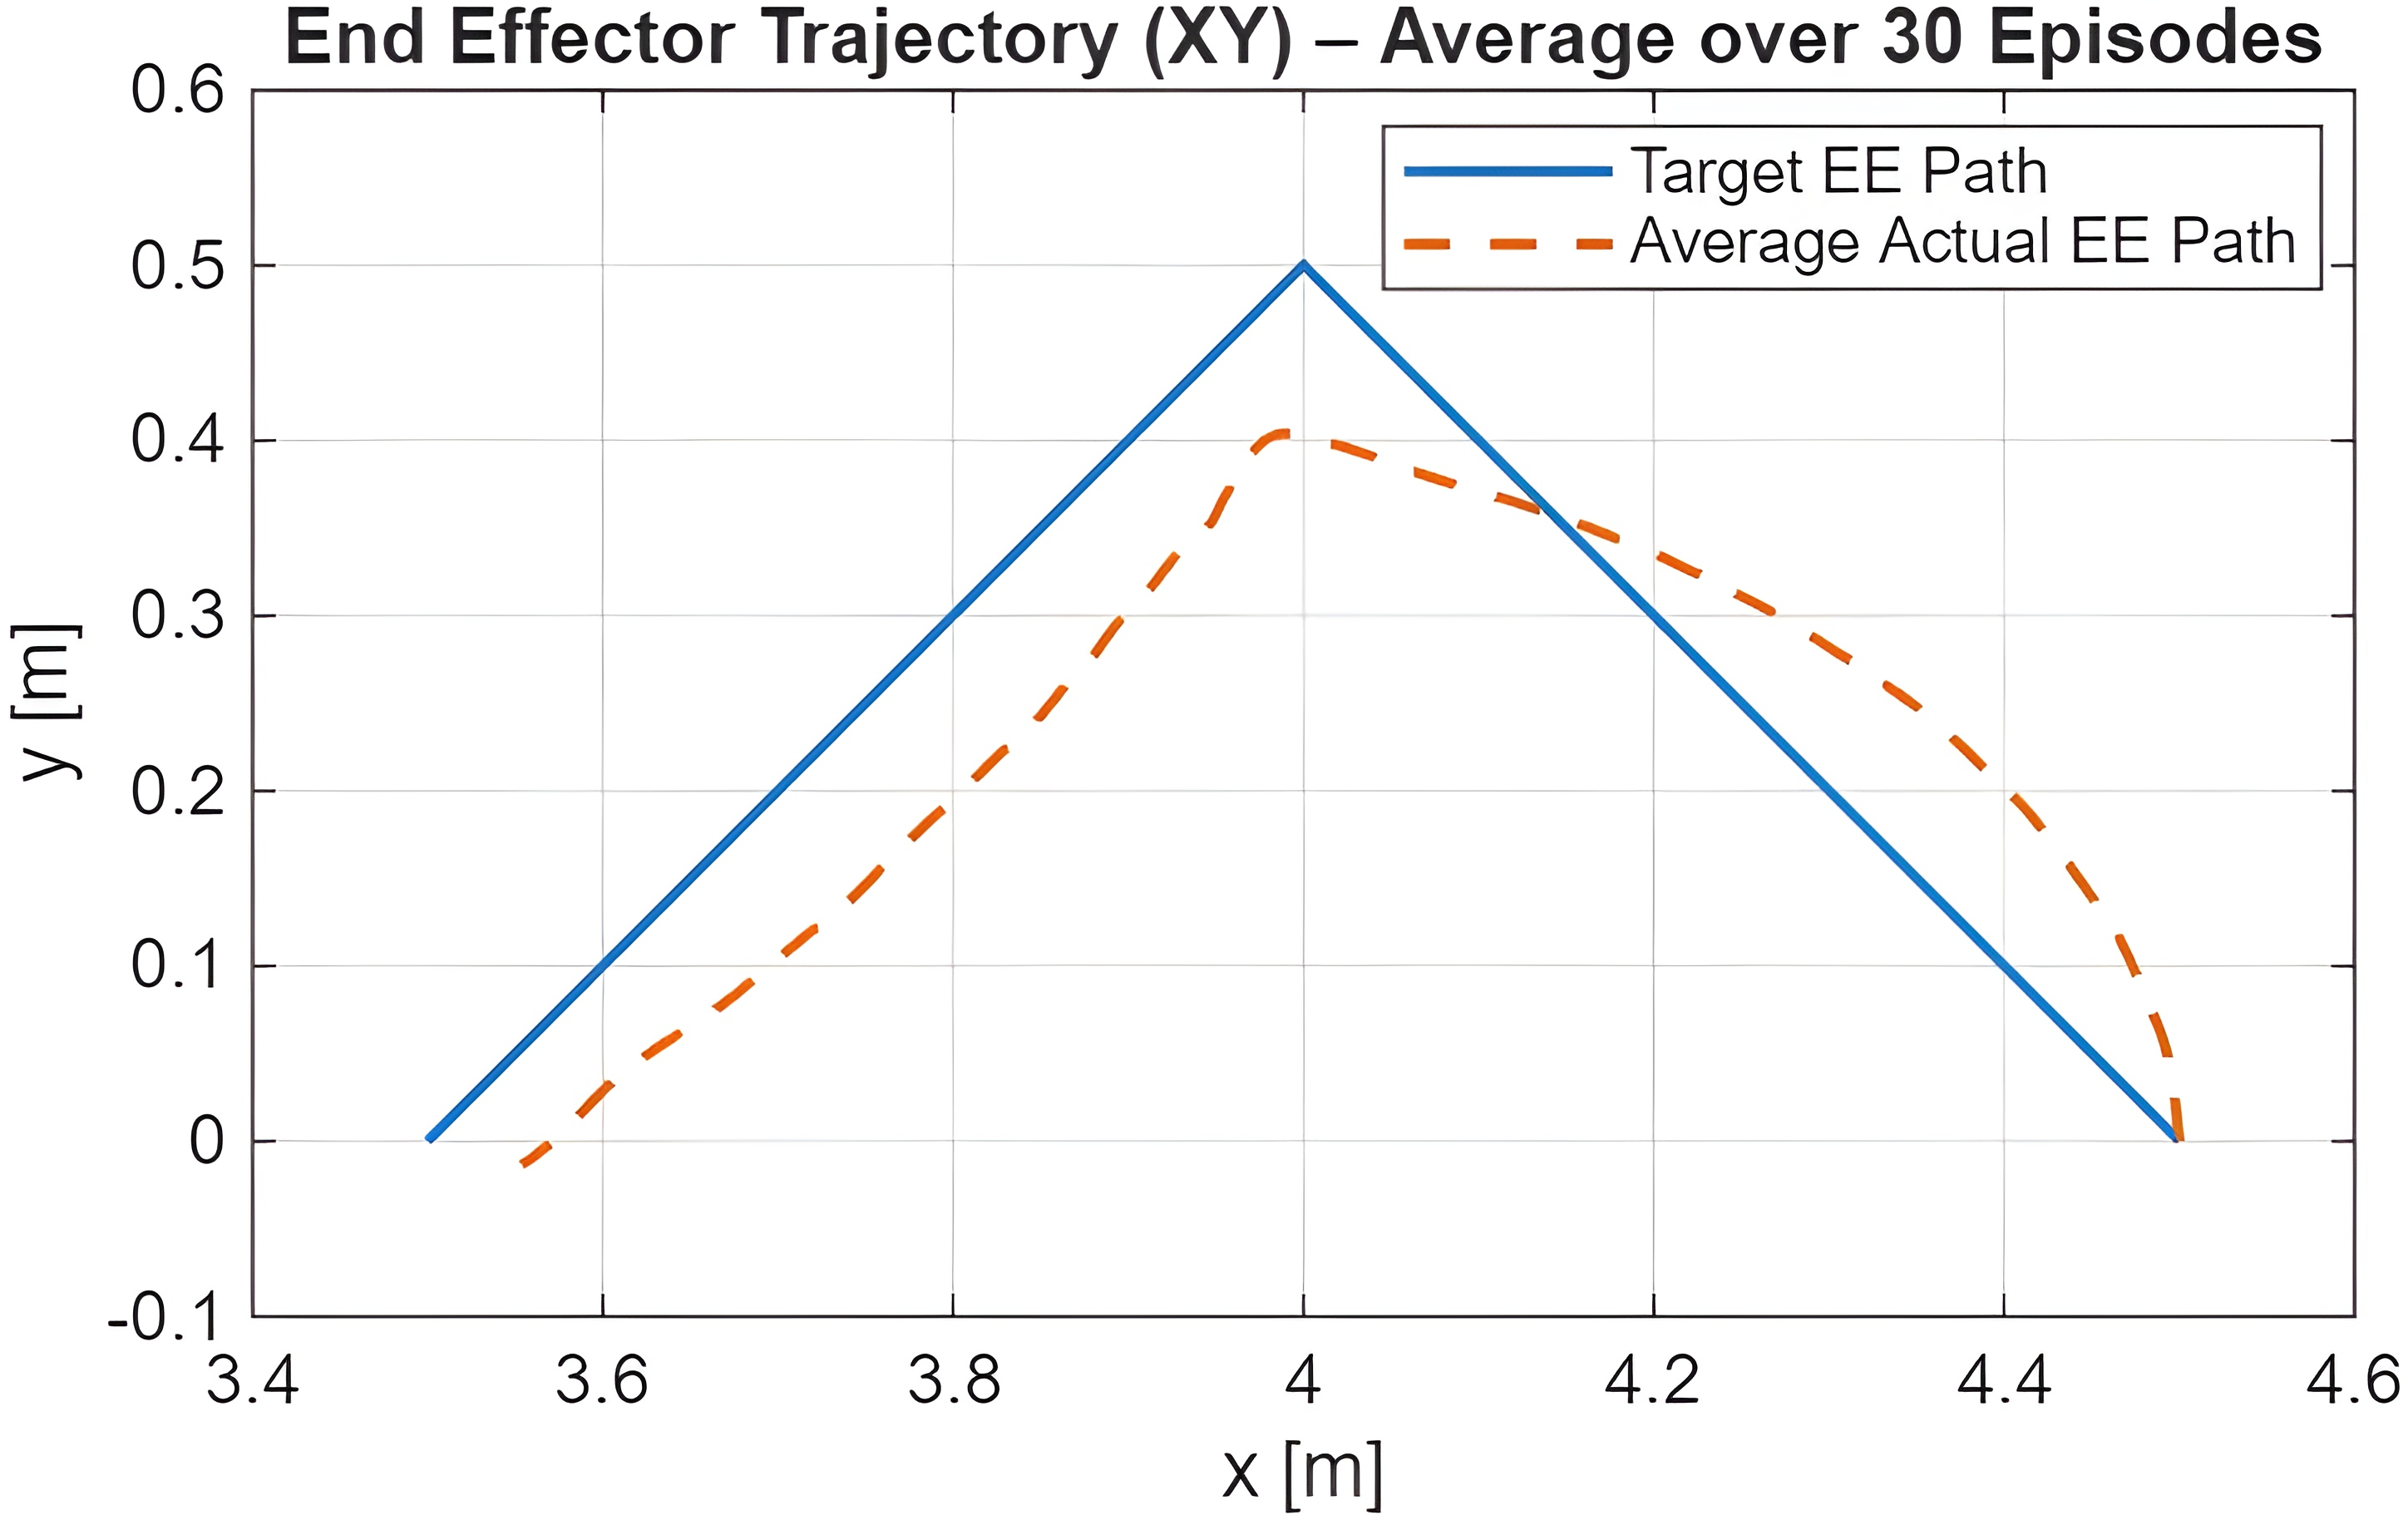
\includegraphics[width=\linewidth]{Figures/rampe_1.png}
        \caption{PPO (default)}
        \label{fig:r_traj_default}
    \end{subfigure}
    \hfill
    \begin{subfigure}{0.48\textwidth}
        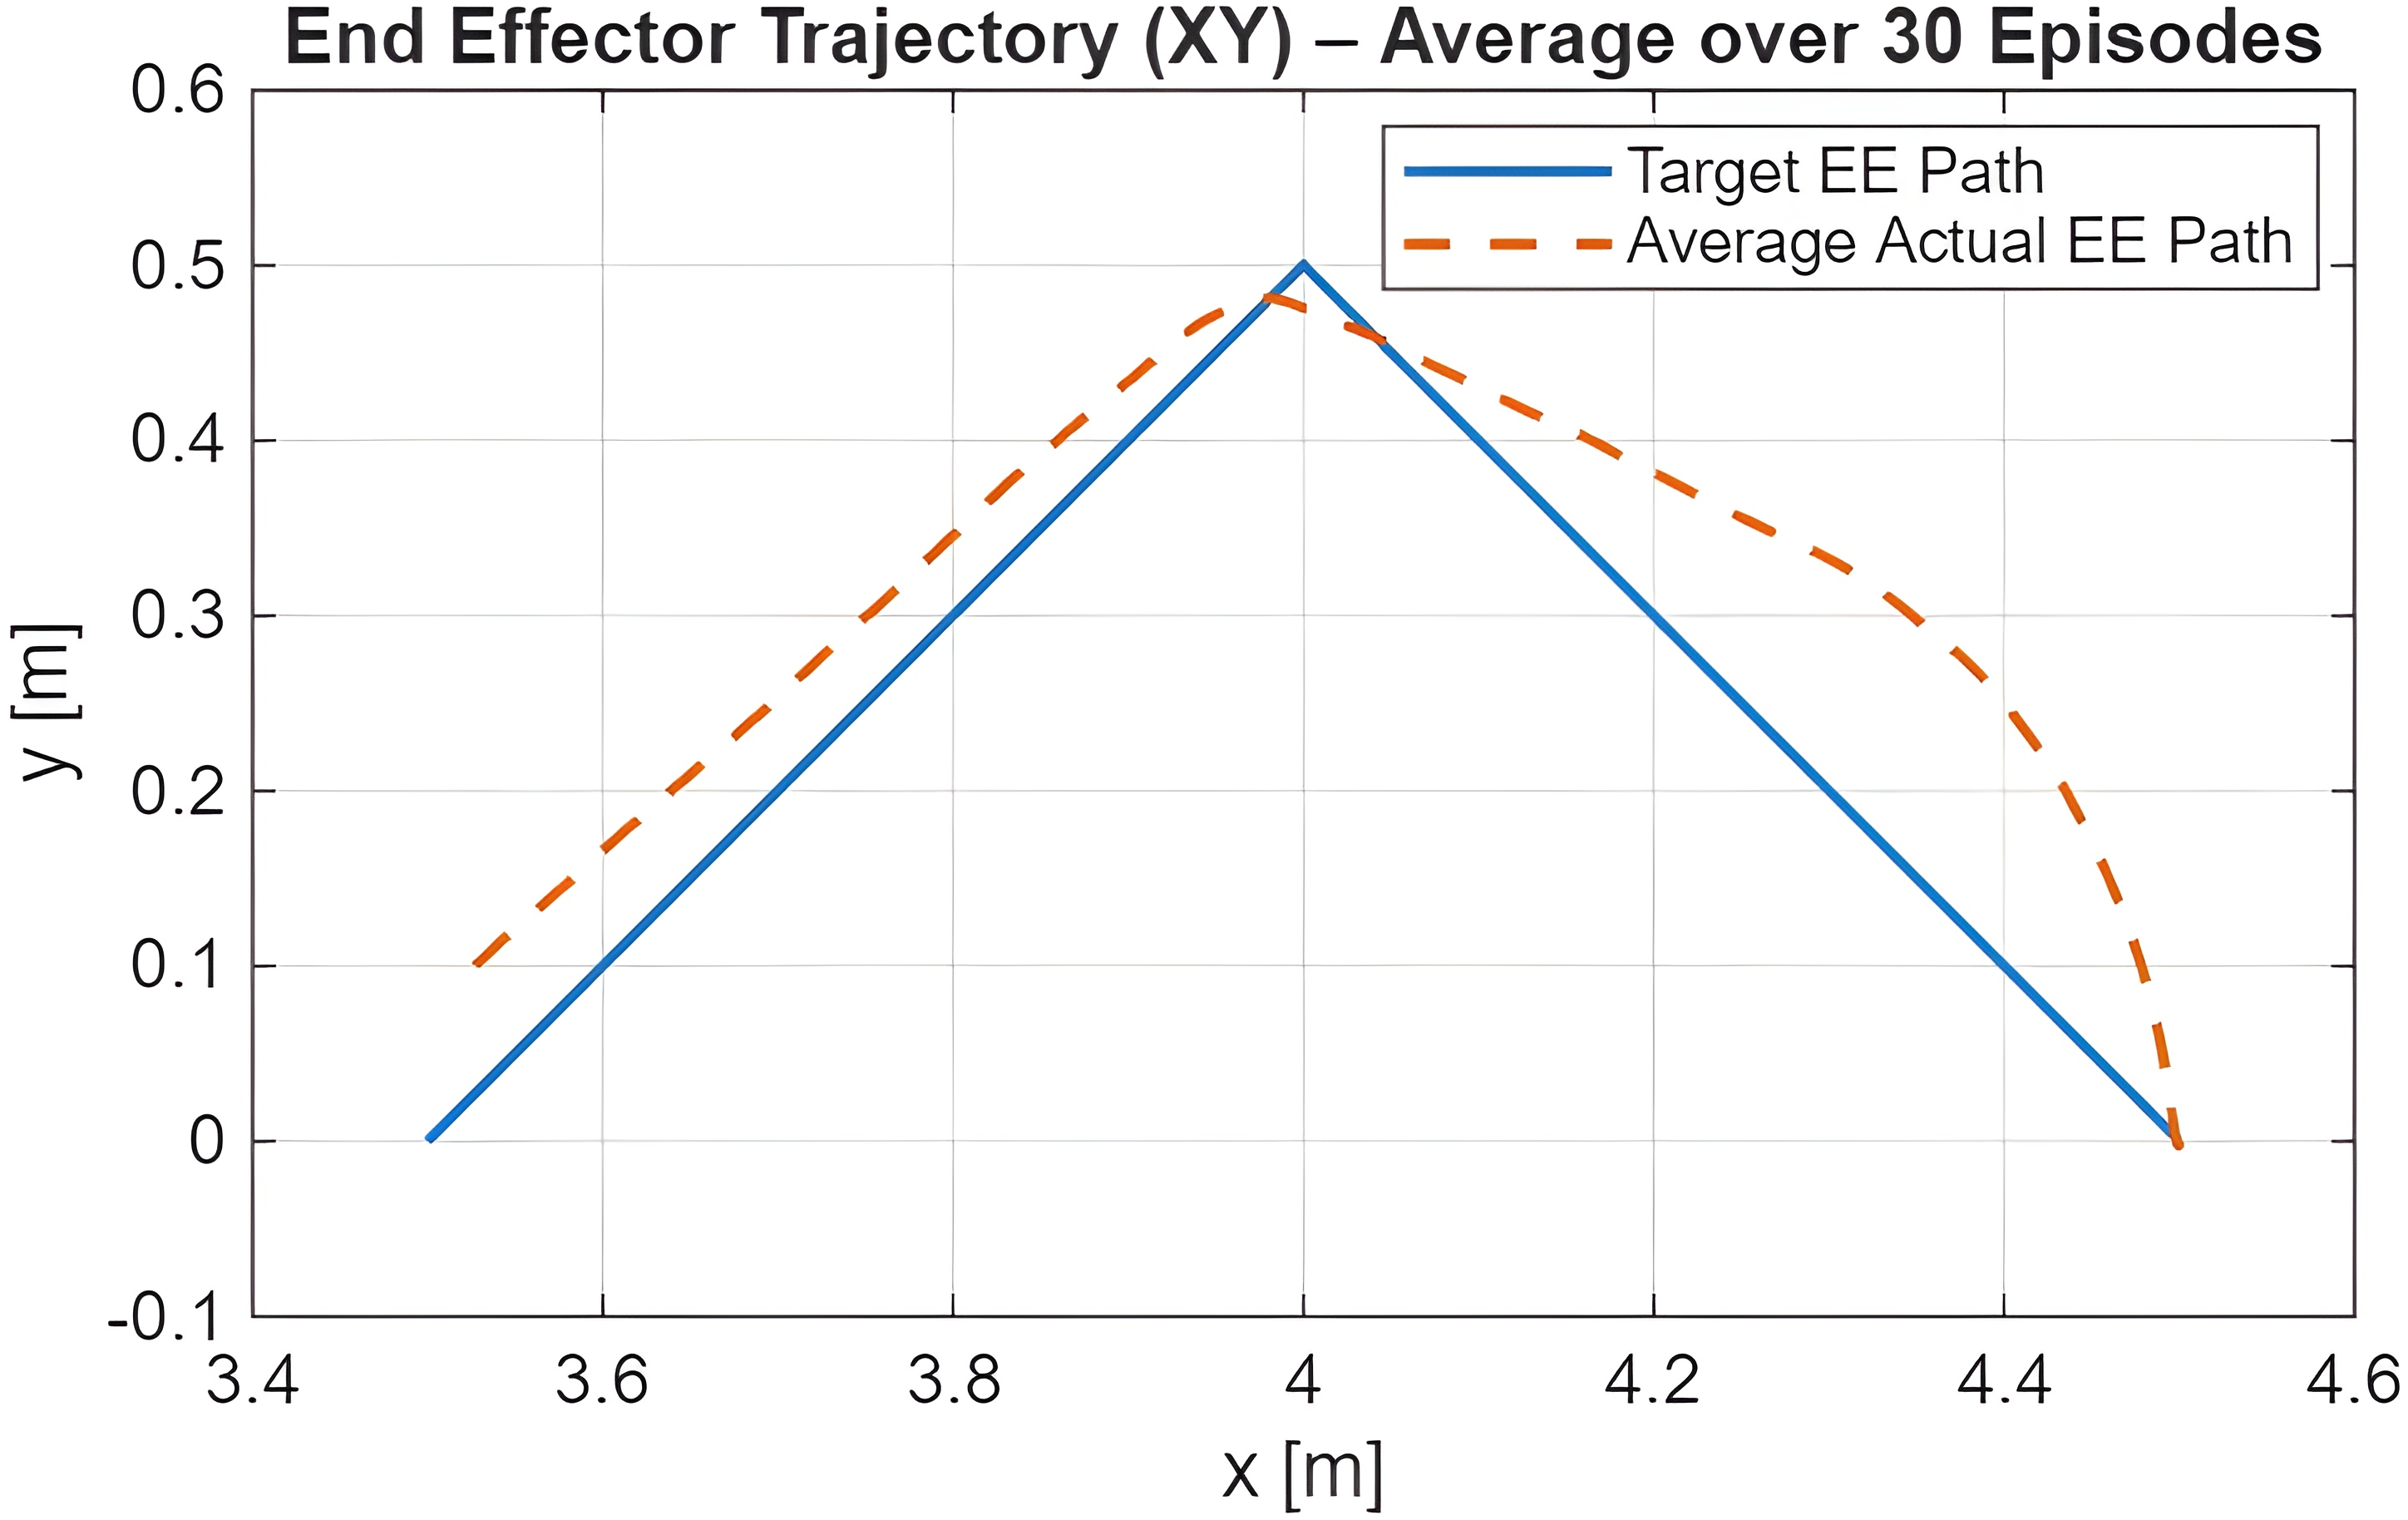
\includegraphics[width=\linewidth]{Figures/rampe_opt_1.png}
        \caption{PPO (optimized)}
        \label{fig:r_traj_opt}
    \end{subfigure}
    \caption{Reference and actual end-effector path on the piecewise-linear reference for one evaluation
    episode from the nominal initial state. The panels show the only successful run of the default PPO agent
    (seed 9) and the run of the optimized PPO agent with the median $K_2$ (seed 5).}
    \label{fig:r_trajektorie_xy_compare}
\end{figure*}

\begin{figure*}[t]
    \centering
    \begin{subfigure}{0.48\textwidth}
        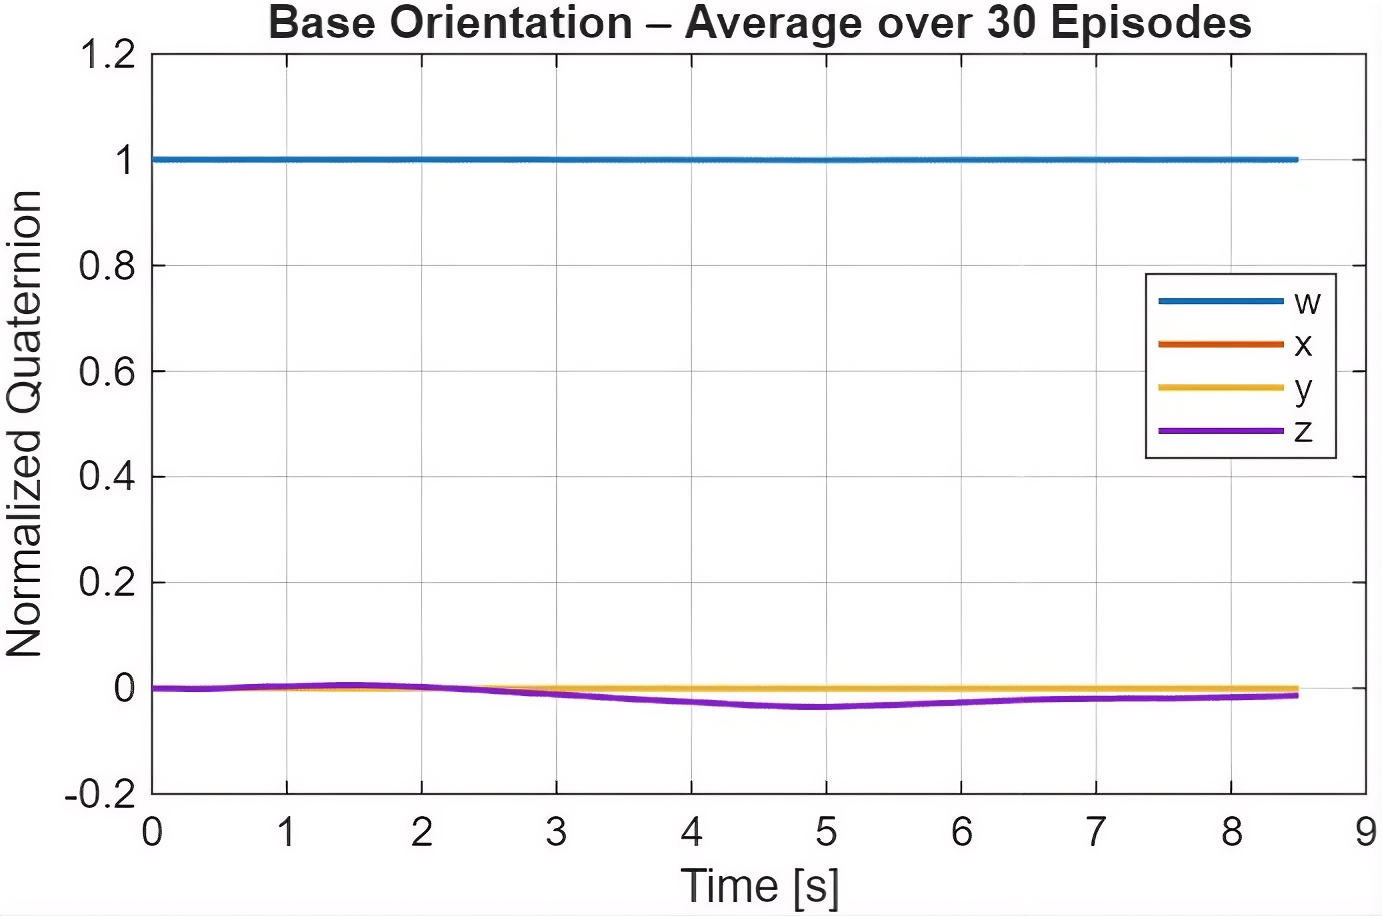
\includegraphics[width=\linewidth]{Figures/basis_ori_1.png}
        \caption{PPO (default)}
        \label{fig:r_basis_default}
    \end{subfigure}
    \hfill
    \begin{subfigure}{0.48\textwidth}
        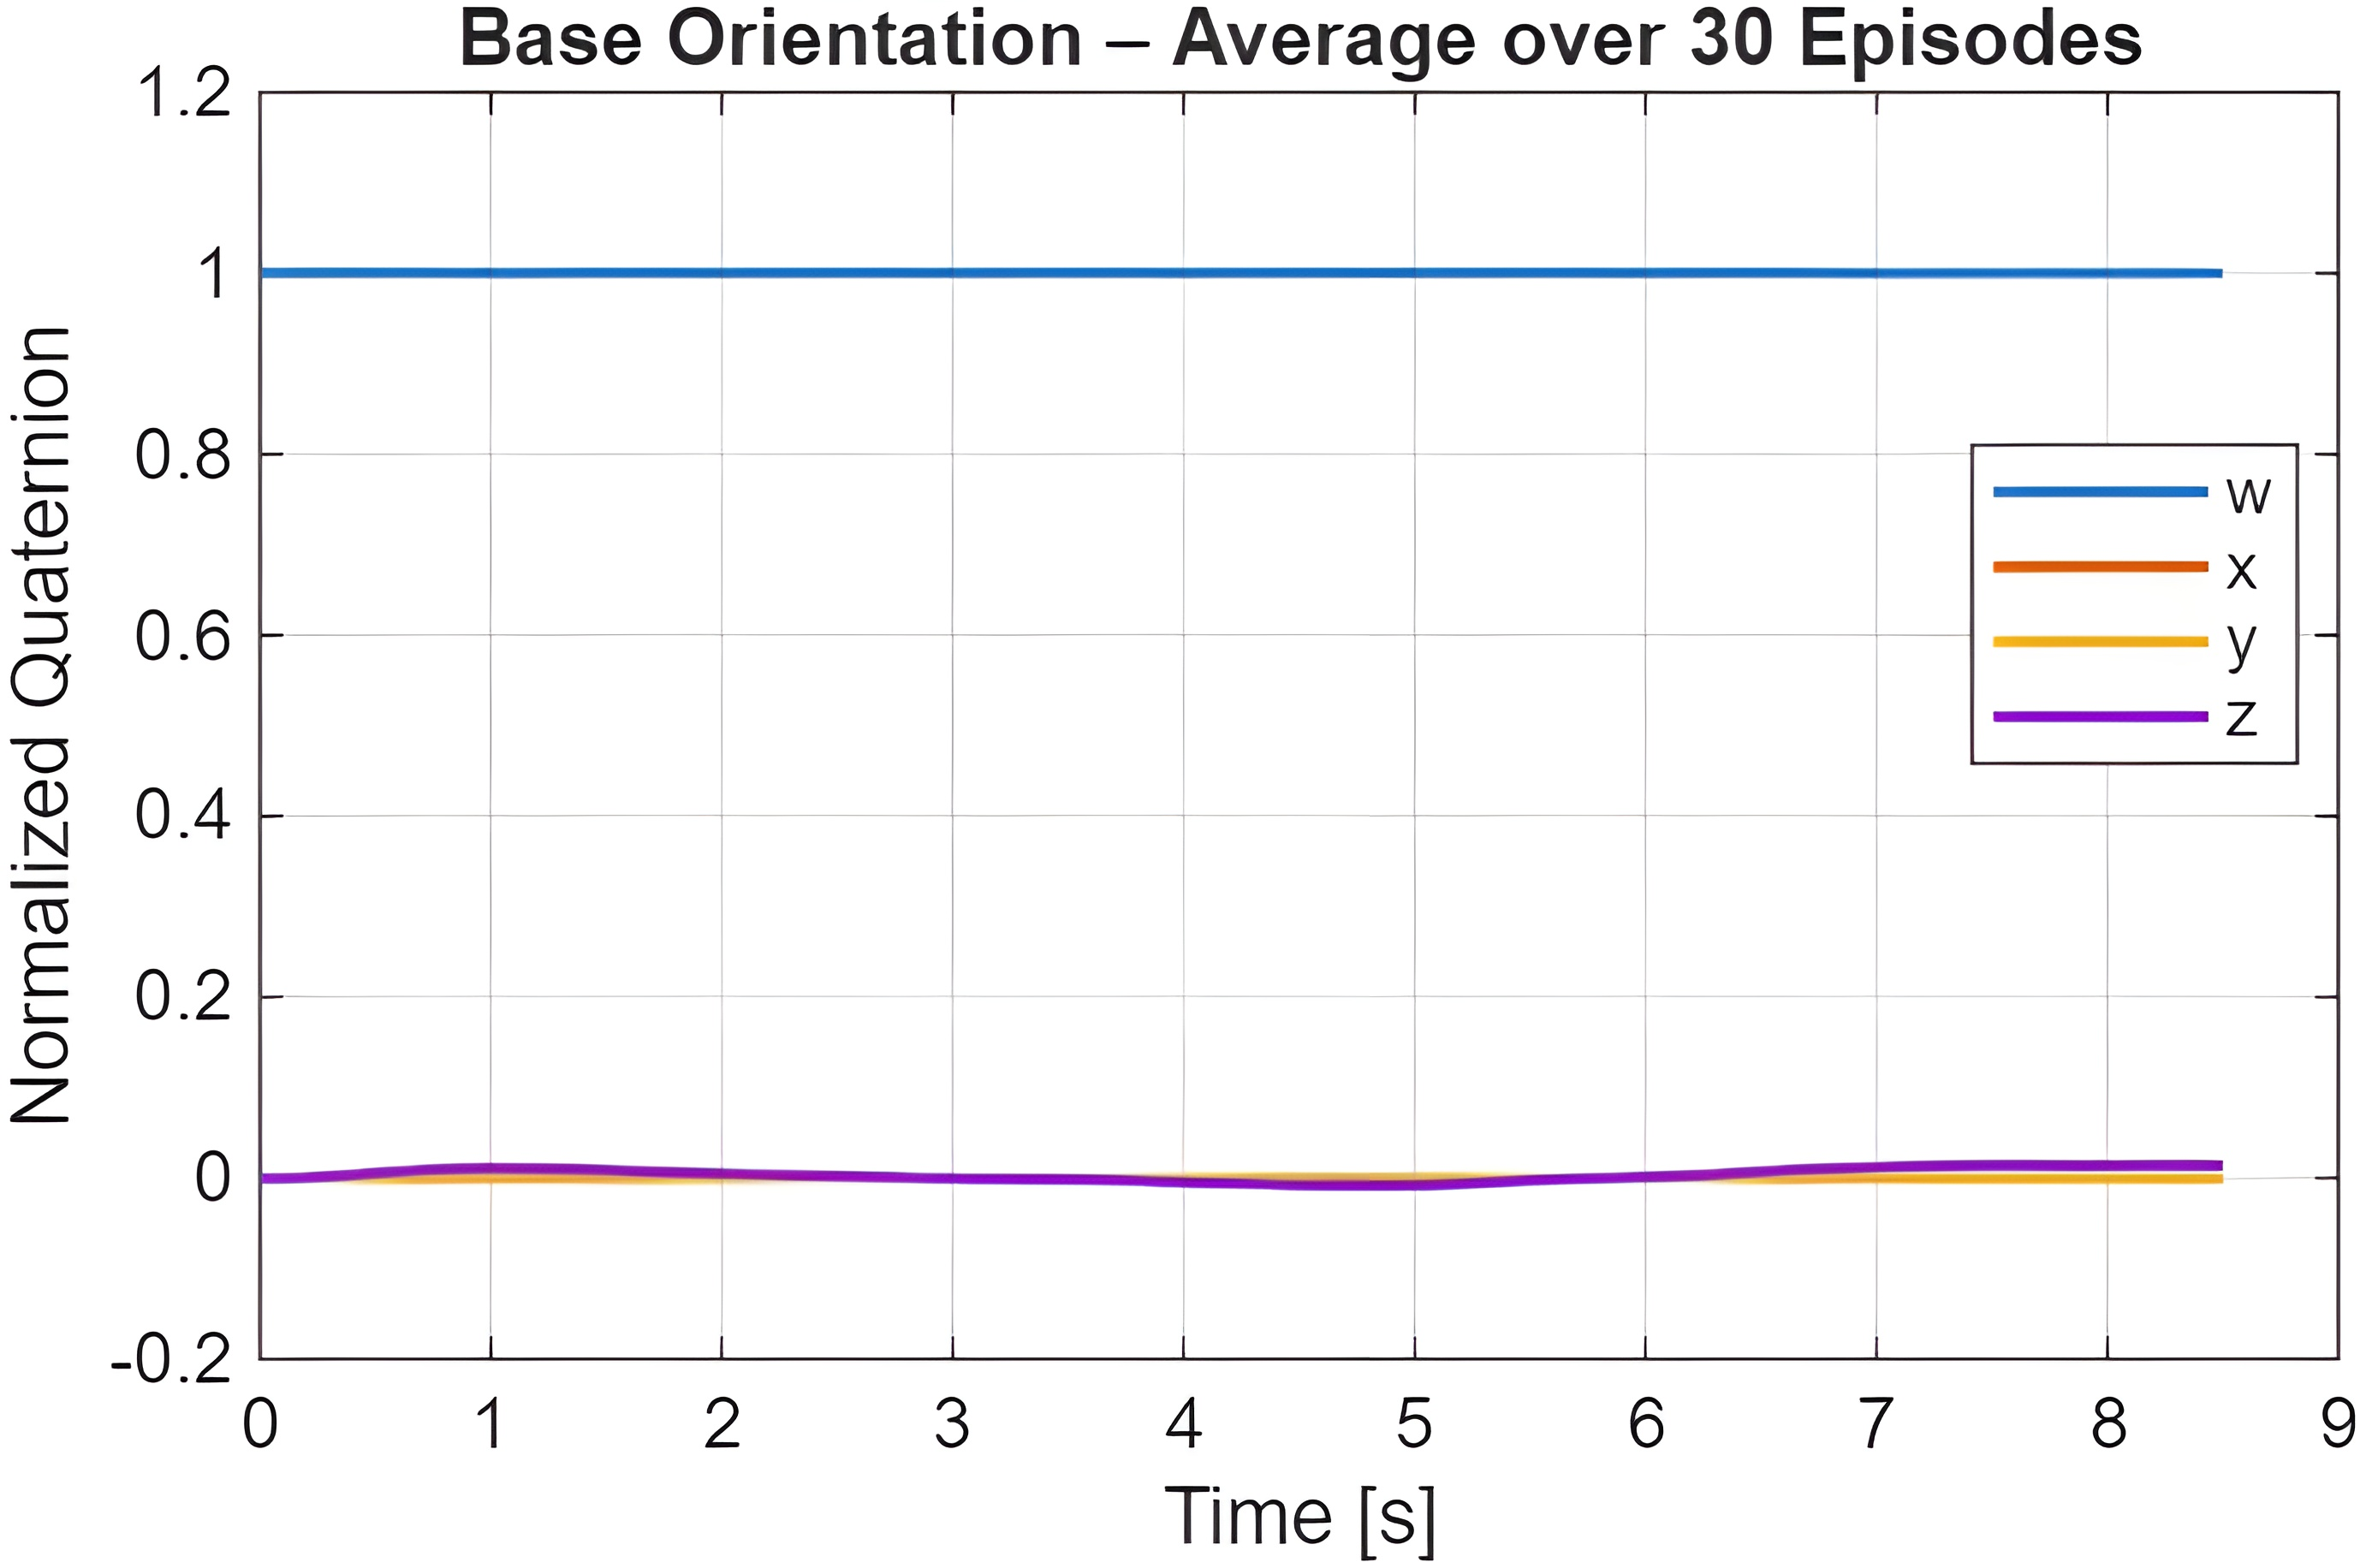
\includegraphics[width=\linewidth]{Figures/basis_ori_opt_1.png}
        \caption{PPO (optimized)}
        \label{fig:r_basis_opt}
    \end{subfigure}
    \caption{Vector part of the base orientation quaternion during the episodes of
    \cref{fig:r_trajektorie_xy_compare}. The base rotates only about the $z$-axis. The scalar part stays above
    0.992 for the default and above 0.999 for the optimized agent.}
    \label{fig:r_basis_orientation_compare}
\end{figure*}

\begin{table*}[t]
\centering
\caption{Default PPO agent, optimized PPO agent, and TRPO on the piecewise-linear trajectory. The first row
gives the number of successful runs out of ten. All other values are the mean and the standard deviation over
the successful runs, which is a single run for the default PPO agent. $K_5$ and $K_6$ are zero for every
successful run and are omitted.}
\label{tab:ppo_linear_kpi}
\renewcommand{\arraystretch}{1.2}
\setlength{\tabcolsep}{8pt}
\begin{tabular}{lccc}
\toprule
\textbf{Metric (KPI)} & \textbf{PPO (default)} & \textbf{PPO (optimized)} & \textbf{TRPO} \\
\midrule
Successful runs & 1/10 & 10/10 & 10/10 \\
Mean Episodic Return ($K_1$) & $-2.43$ & $-0.19 \pm 0.15$ & $-0.41 \pm 0.37$ \\
Mean Squared EE Position Error ($K_2$) & $0.0528$ & $0.0059 \pm 0.0053$ & $0.0125 \pm 0.0105$ \\
Maximum EE Position Error ($K_3$) & $0.415$ & $0.150 \pm 0.013$ & $0.194 \pm 0.055$ \\
Mean Base Orientation Error ($K_4$) & $0.129$ & $0.019 \pm 0.011$ & $0.029 \pm 0.023$ \\
Control Smoothness ($K_7$, Jerk) & $0.402$ & $0.0117 \pm 0.0019$ & $0.0105 \pm 0.0029$ \\
Mean Base Angular Velocity ($K_8$) & $0.048$ & $0.013 \pm 0.006$ & $0.020 \pm 0.010$ \\
Energy Consumption ($K_9$) & $11.8$ & $3.42 \pm 1.85$ & $2.49 \pm 1.26$ \\
Reward Std.\ (Late Training, $T_1$) & $3.55$ & $0.12 \pm 0.11$ & $0.94 \pm 1.37$ \\
Training Time ($T_2$, min) & $6.08$ & $7.30 \pm 0.04$ & $8.60 \pm 0.11$ \\
\bottomrule
\end{tabular}
\end{table*}

\textbf{Results.} \cref{tab:ppo_linear_kpi} summarizes the results on the piecewise-linear reference. The
optimized PPO agent and TRPO completed all ten runs without a terminated episode, whereas the default PPO
agent succeeded in only one run (Fisher's exact test against TRPO, $p < 0.001$). Over the successful runs,
the optimized PPO agent reached a mean squared tracking error of $K_2 = 0.0059$, compared with 0.0125 for
TRPO. On the seed level, the optimized PPO agent had a higher return and lower mean and maximum tracking
errors than TRPO, with uncorrected $p$-values between 0.026 and 0.038 ($K_1$, $K_2$, and $K_3$,
Mann--Whitney). The difference in the base orientation error had $p = 0.054$ ($K_4$, 0.019 compared with
0.029). After a Holm correction over the seven tested KPIs, none of these differences was significant.

\cref{fig:r_trajektorie_xy_compare} shows the end-effector path of one episode for the default and the
optimized PPO agent. The only successful run of the default agent lags behind the reference, oscillates
along both segments, and ends far from the final point. The optimized agent approaches the first segment on
a curved path, cuts the corner, and then follows the second segment closely.
\cref{fig:r_basis_orientation_compare} shows the corresponding base orientations. The largest vector
component of the quaternion was 0.121 for the default and 0.039 for the optimized agent.

Under the tested conditions, the configurations of TRPO and the optimized PPO agent carried over to the
piecewise-linear path without changes. As on the circular path, the optimized agent had a lower mean
tracking error than TRPO, but the difference was not significant after the correction. The default PPO
agent succeeded in only one of ten runs.

The following section discusses the implications, limitations, and future steps toward deployment on physical
testbeds for space robotics.

\section{Discussion and Conclusion}\label{sec:discussion} This work investigated continuous-action deep
RL for the control of a free-floating space robotic arm, with a focus on control performance and the
monitored safety properties. The main observation is that no RL algorithm is universally superior. The
benchmark indicates that bounding the size of policy updates is important when Cartesian tracking,
stabilization of the base attitude, and constraint satisfaction are coupled in a free-floating robot
system.

The results show that an RL-based controller can perform the desired manipulation task in the simulated
space environment under the considered assumptions. With the toolbox default hyperparameters, the agents
differed more in how often training succeeded than in the performance of their successful runs. TRPO
completed all ten runs, whereas the other default agents terminated 40.0\% to 80.0\% of their evaluation
episodes. The tuned PPO agent also completed all runs. It reached a mean squared tracking error of
$K_2 = 0.0041$, compared with 0.0145 for TRPO and 0.0134 for the successful runs of the default PPO
agent. Its advantage over TRPO was not statistically significant, but it trained faster. No violations
of the monitored safety properties were recorded for TRPO and the tuned PPO agent in any evaluation
episode.

An additional evaluation on a piecewise-linear end-effector reference tested whether the configurations
carry over to a different path. With the same hyperparameters and reward weights, the optimized PPO agent
and TRPO again completed all ten runs. The optimized agent again had a lower mean tracking error than
TRPO ($K_2$, 0.0059 compared with 0.0125), but the difference was not significant after a correction
over the tested KPIs. The default PPO agent succeeded in only one of ten runs. The ablation and the
sensitivity analysis indicate that $W_p$ and $W_{\mathrm{ori}}$ dominate the reward design. When these
weights were halved or doubled, TRPO kept the most successful runs and the lowest tracking error of the
three retrained algorithms. The order of the default PPO agent and SAC was not stable across the
variants. In the stress tests, TRPO and the optimized PPO agent completed all runs under sensor noise,
reduced torque limits, an external joint torque, and uniformly scaled masses, inertias, and damping. The
uniform scaling acts like weaker actuators and increased their tracking errors by a factor of two to
three. These results are limited to a few perturbation levels and two reference paths.

\textbf{Practical Implications.} The results of TRPO and the tuned PPO agent indicate that
policy-gradient methods with constrained updates are suitable candidates for continuous control tasks
with strong dynamic coupling and safety constraints. For PPO, this held only with a smaller learning rate
than the toolbox default. With the default learning rate of $10^{-2}$, the clipped surrogate objective of
PPO did not prevent the seed dependence observed in \cref{comparison}. The runtime monitors (collision
monitor and joint-limit monitor) supervise the training. They terminate episodes in which the policy
would violate a monitored constraint and apply a terminal penalty. Combined with the penalty-driven
reward, this led to final policies of TRPO and the tuned PPO agent that did not violate the monitored
constraints in the reported evaluation. The present simulation study does not establish that this
behavior transfers to a physical system. It suggests only that safety checks embedded in the training
simulator may remain useful as runtime watchdogs, provided that the deployed system stays within the
simulator's fidelity range, which remains to be validated.


\textbf{Limitations and Future Work.} The study has several limitations. First, a \emph{sim-to-real gap}
remains. Beyond the idealizing assumptions stated in \cref{sec:sim} (no sensor noise, no latency,
rigid-body model, no external disturbances), real deployment introduces three further challenges. The
first is a \emph{domain shift} due to inaccurate mass and inertia parameters, joint friction, and link
flexibility, which the URDF model does not capture. The second concerns \emph{onboard compute
constraints}. The learned policy must run in real time on embedded space-qualified hardware, typically
ARM-based processors with limited floating-point throughput, whereas training was performed on a
workstation CPU. The third is \emph{sensor--actuator latency}. Delays between state measurement and
torque application can destabilize a policy that was trained without latency. Mitigating these effects
would require domain randomization over simulation parameters, latency injection during training, and
ultimately HIL validation~\cite{b8}.

Second, the RL agent exhibits \emph{hyperparameter sensitivity}. The tuned PPO configuration is
task-specific and may require re-tuning for different trajectories or mission scenarios. It was selected
in an earlier grid search with a single run per candidate. It also differs from the default agent in the
output layer of the policy mean, which has no tanh bound, and the effects of the two changes were not
separated. The other algorithms were compared only with their toolbox default hyperparameters, and
tuning them might change their ranking.

Third, the \emph{evaluation scope} is limited. Each configuration was trained with ten seeds and
evaluated on 31 initial states within $\pm 1^\circ$ of the nominal pose, for a single robot model and
two reference paths. Both paths lie in one plane, and all joint axes are parallel, so the task is planar
and the base rotates about a single axis. Out-of-plane motion and three-axis base rotation were not
tested. Ten runs per configuration allow only coarse estimates of the success rate, and the KPIs of
agents with few successful runs rest on two to four runs. The stress tests cover a small set of
perturbations. The reported ranking and improvements are therefore conditional on the tested setup.
The comparison is mainly evidence of how robust training is to the choice of seed in this setup. It is
not a definitive ranking of all considered RL algorithms.

Fourth, the \emph{state representation} was manually designed. Learned representations or recurrent
architectures (LSTM) might improve performance under partial observability. Fifth, the \emph{safety
monitoring} covers selected properties (collision events, joint limits, torque bound, and momentum
consistency). Only the torque bound of the actuation path is checked formally, and the other properties
are monitored at runtime. The safety components do not constitute a formal proof of closed-loop
stability, task completion, or collision avoidance for the full nonlinear model, nor an exhaustive
formal verification of the mission. Finally, \emph{no hardware testing} was performed. Real-time
computation limits, communication delays, and physical interactions remain to be validated on physical
testbeds.

Future work could address these limitations in four directions. The first is domain randomization over
simulation parameters and latency injection to improve the sim-to-real transfer~\cite{b8} (see
\cref{fig:oos}). The second is the extension to more complex tasks such as three-dimensional motion,
dual-arm coordination, on-orbit assembly, or active debris removal. The third is the use of recurrent
policies, attention mechanisms, and safe RL algorithms with explicit constraint handling via Lagrange
multipliers or barrier functions~\cite{b22,b24,b23,b34}. The fourth is HIL validation on the authors'
testbed for in-space robotized services with virtually simulated microgravity and predicted energy
consumption (see \cref{fig:oos}).


\textbf{Conclusion.} This work has presented a framework that combines deep reinforcement learning,
multibody simulation, runtime safety monitoring, and a formal check of the torque bound for planar
Cartesian path tracking of a free-floating space robot. Six continuous-action RL algorithms were
compared under unified conditions with the toolbox default hyperparameters and ten seeds each. For the
considered simulated task and evaluation setup, TRPO was the only default agent that completed all runs
without a safety abort. A tuned PPO configuration also completed all runs and reached the lowest tracking
error with a shorter training time than TRPO, although this difference was not statistically
significant. The runtime monitors in the training loop detected the violations of the monitored
constraints by the other agents and terminated the affected episodes. The formal check showed that the
actuation path bounds the commanded torques for any policy output. These simulation results, obtained
under the stated idealizing assumptions, do not establish formal safety or operational readiness, but
they support further investigation of deep RL with runtime safety monitoring for space manipulation
tasks.

The results also illustrate the influence of algorithm choice and hyperparameter tuning on the learning
performance for the considered task. They are consistent with the view that no single RL algorithm
is uniformly best across applications. Under unified conditions, the choice of algorithm and hyperparameters
visibly affected the achieved tracking accuracy and base stability and, above all, how often
training succeeded. Systematic benchmarking of candidate algorithms over several seeds is
therefore a practical step in the selection of an appropriate RL controller for a given task.

Several open problems remain for real-world deployment, but the proposed framework provides a basis
for further investigation. Possible application areas include satellite servicing, on-orbit assembly, and active
debris removal, in which learning-based controllers could adapt to uncertain dynamics within predefined
operational limits. One possible architecture for such applications combines an RL policy with a separate runtime
layer that monitors the commands and overrides those that violate the specified constraints. In this combination,
the learned policy provides adaptability, while the monitoring layer detects and intercepts violations of the
specified properties, similar to the shielding approach in~\cite{b23}.

%\begin{figure}[!t]
%	\centering
%	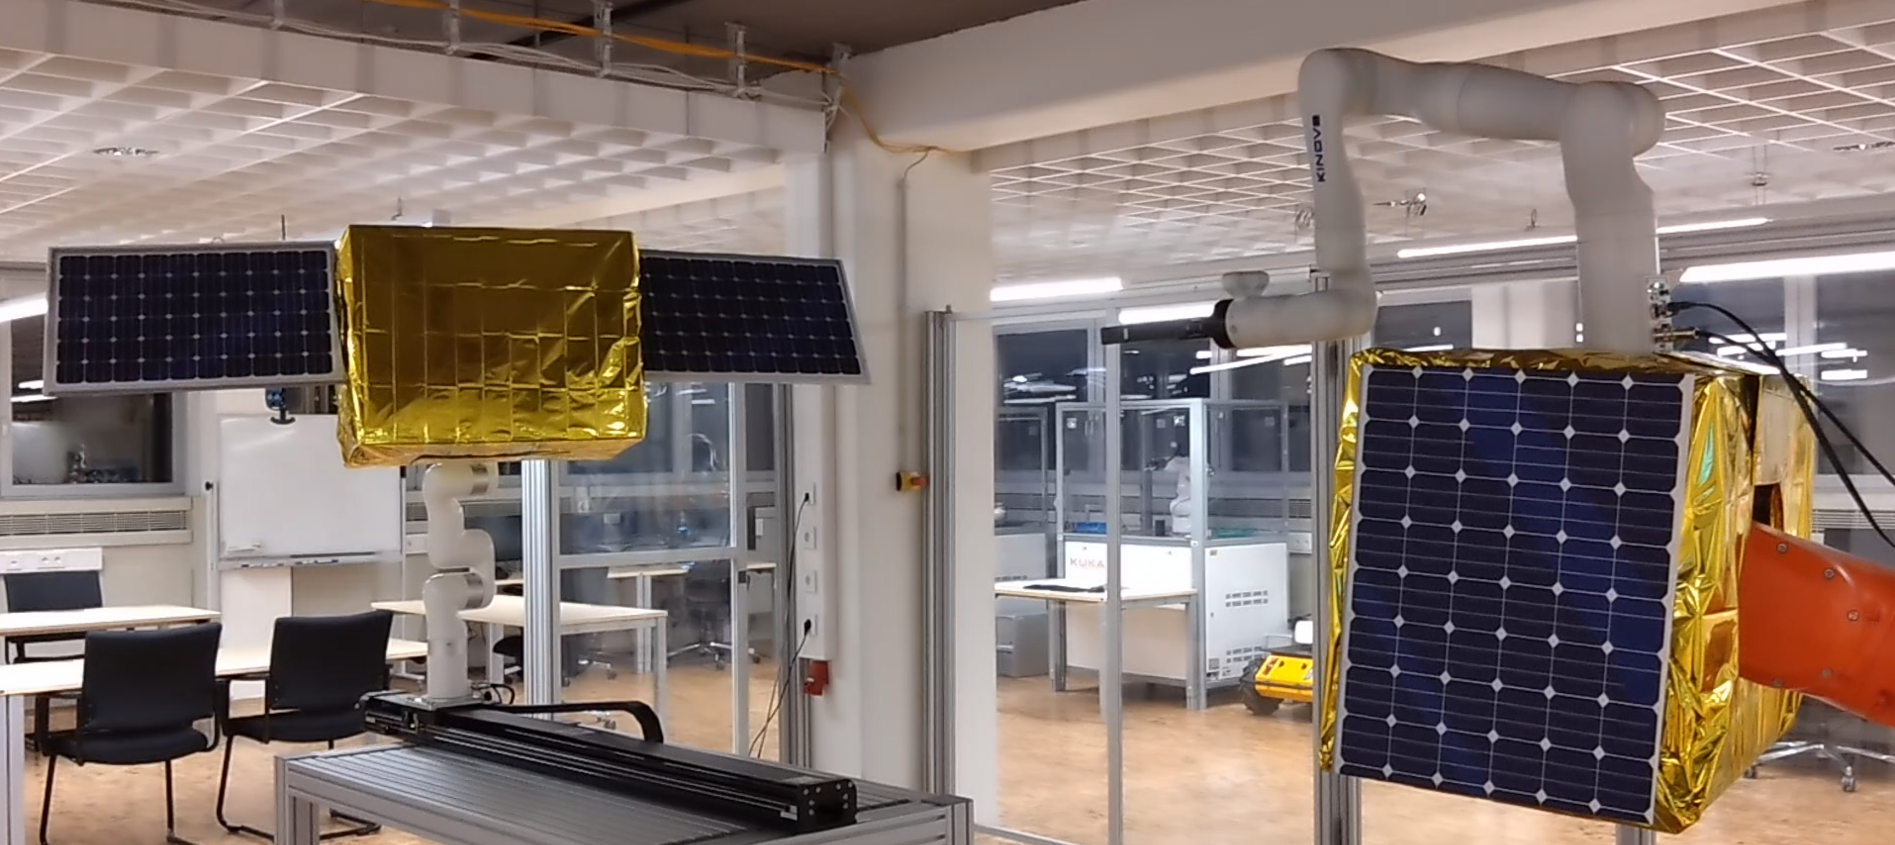
\includegraphics[width=0.8\linewidth]{Figures/testbed.png}
%	\caption{Our testbed for In-Space Robotized Services.}
%	\label{fig:physicaltestbed}
%\end{figure}

This work is one step in this direction. Future research at the intersection
of robotics, reinforcement learning, and formal methods is required to extend the present results
to physical deployment and to broader mission scenarios.

\section*{Acknowledgment}
The authors used DeepL Translator/Write and OpenAI ChatGPT
for language editing and grammar enhancement. The illustration in \cref{fig:oos} was generated with
GPT-Image-2 (OpenAI) from a photograph of the physical setup.
\begin{thebibliography}{00}

\bibitem{b1} A. Flores-Abad, O. Ma, K. Pham, and S. Ulrich, ``A review of space robotics technologies for
on-orbit servicing,'' \emph{Prog. Aerosp. Sci.}, vol.~68, pp. 1--26, 2014, doi:
10.1016/j.paerosci.2014.03.002.



\bibitem{b6}
K. Nanos and E. G. Papadopoulos, ``On the dynamics and control of free-floating space
manipulator systems in the presence of angular momentum,'' \emph{Front. Robot. AI}, vol.~4, p.~26, 2017,
doi: 10.3389/frobt.2017.00026.



\bibitem{b11}
E. Papadopoulos, I. Kaliakatsos, and D. Psarros, ``Minimum fuel techniques for a space robot
simulator with a reaction wheel and PWM thrusters,'' in \emph{Proc. Eur. Control Conf. (ECC)},
2007, pp. 3391--3398.



\bibitem{b32}
E. Papadopoulos and A. Abu-Abed, ``Design and motion planning for a zero-reaction manipulator,'' in
\emph{Proc. IEEE Int. Conf. Robot. Autom. (ICRA)}, 1994, pp. 1554--1559, doi: 10.1109/ROBOT.1994.351367.



\bibitem{muhlbauer2025software}
M. M{\"u}hlbauer, M. Chalon, M. Ulmer, and A. Albu-Sch{\"a}ffer, ``Software for the SpaceDREAM robotic
arm,'' in \emph{Proc. IEEE Aerosp. Conf.}, 2025.



\bibitem{rybus2024robotic}
T. Rybus, ``Robotic manipulators for in-orbit servicing and active debris removal: Review and comparison,''
\emph{Prog. Aerosp. Sci.}, vol.~151, p.~104550, 2024.



%\bibitem{maurenbrecher2024robograv}
%H. Maurenbrecher \emph{et al.}, ``RoboGrav---Towards force sensitive space manipulators,'' in \emph{Proc. I-SAIRAS}, 2024.

\bibitem{kaigom2011optimal}
E. Guiffo Kaigom, T. Jung, and J. Roßmann, ``Optimal motion planning of a space
robot with base disturbance minimization,'' in \emph{Proc. 11th Symp. Adv. Space Technol. Robot. Autom.},
2011.

\bibitem{kaigom2025deep}
E. Guiffo Kaigom, ``Deep generative and discriminative digital twin endowed with variational autoencoder for
unsupervised predictive thermal condition monitoring of physical robots in Industry 6.0 and Society 6.0,''
\emph{IFAC-PapersOnLine}, vol.~59, pp. 7--12, 2025.

\bibitem{la2025deep}
T. K. La and E. Guiffo Kaigom, ``Deep learning for model-free prediction of thermal states of robot joint
motors,'' \emph{IFAC-PapersOnLine}, vol.~59, no.~18, pp. 211--216, 2025.

\bibitem{huang2023obstacle} Z. Huang, G. Chen, Y. Shen, R. Wang, C. Liu, and L. Zhang, ``An
obstacle-avoidance motion planning method for redundant space robot via reinforcement learning,''
\emph{Actuators}, vol.~12, no.~2, p.~69, 2023.



\bibitem{al2024reinforcement} A. Al Ali and Z. Zhu, ``Reinforcement learning for path planning of
free-floating space robotic manipulator with collision avoidance and observation noise,'' \emph{Front.
Control Eng.}, vol.~5, p.~1394668, 2024.



\bibitem{d2024failure}
M. D'Ambrosio, L. Capra, A. Brandonisio, and M. Lavagna, ``Failure management via deep reinforcement
learning for robotic in-orbit servicing,'' in \emph{Proc. SPAICE---1st Joint ESA/IAA Conf. AI Space}, 2024,
pp. 335--339.



\bibitem{al2024path}
A. Al Ali, J. Shi, and Z. Zhu, ``Path planning of 6-DOF free-floating space
robotic manipulators using reinforcement learning,'' \emph{Acta Astronaut.}, vol.~224, pp. 367--378, 2024.



\bibitem{hu2025deep} Y. Hu, D. Zhou, W. Yao, X. Shao, and G. Sun, ``Deep reinforcement learning-based
trajectory planning with continuous pose representation for 6-DoF free-floating space robot,''
\emph{Aerosp. Sci. Technol.}, p.~110540, 2025.



\bibitem{zhang2025learning} O. Zhang, Z. Liu, X. Shao, W. Yao, L. Wu, and J. Liu, ``Learning-based task
space trajectory planning framework with pre-planning and post-processing for uncertain free-floating
space robots,'' \emph{IEEE Trans. Aerosp. Electron. Syst.}, early access, 2025.



\bibitem{wei2025trajectory} Y. Wei, X. Bai, and H. Lu, ``Trajectory planning of free-floating space robot
for non-cooperative tumbling target capture based on deep reinforcement learning,'' \emph{Robotica},
vol.~43, pp. 2674--2692, 2025.



\bibitem{wu2020reinforcement}
Y. Wu, Z. Yu, C. Li, M. He, B. Hua, and Z. Chen, ``Reinforcement
learning in dual-arm trajectory planning for a free-floating space robot,'' \emph{Aerosp. Sci. Technol.}, vol.~98,
p.~105657, 2020.



\bibitem{b14}
J. Schulman, S. Levine, P. Abbeel, M. Jordan, and P. Moritz, ``Trust region policy
optimization,'' in \emph{Proc. Int. Conf. Mach. Learn. (ICML)}, 2015, pp. 1889--1897.



\bibitem{b17}
S. Fujimoto, H. van Hoof, and D. Meger, ``Addressing function approximation error in actor-critic
methods,'' in \emph{Proc. Int. Conf. Mach. Learn. (ICML)}, 2018, pp. 1587--1596.



\bibitem{b18}
T. Haarnoja, A. Zhou, P. Abbeel, and S. Levine, ``Soft actor-critic: Off-policy maximum entropy
deep reinforcement learning with a stochastic actor,'' in \emph{Proc. Int. Conf. Mach. Learn. (ICML)},
2018, pp. 1861--1870.



\bibitem{b15}
J. Schulman, F. Wolski, P. Dhariwal, A. Radford, and O. Klimov, ``Proximal policy optimization
algorithms,'' arXiv:1707.06347, 2017.



\bibitem{b21} R. J. Williams, ``Simple statistical gradient-following algorithms for connectionist
reinforcement learning,'' \emph{Mach. Learn.}, vol.~8, pp. 229--256, 1992.



\bibitem{b7}
R. S. Sutton and A. G. Barto, \emph{Reinforcement Learning: An Introduction}, 2nd~ed. Cambridge, MA,
USA: MIT Press, 2018.



\bibitem{b5} MathWorks, ``Simulink Design Verifier,'' MATLAB \& Simulink Documentation, 2024. [Online].
Available: \url{https://www.mathworks.com/help/sldv/}



\bibitem{b22} J. Garc{\'\i}a and F. Fern{\'a}ndez, ``A comprehensive survey on safe reinforcement
learning,'' \emph{J. Mach. Learn. Res.}, vol.~16, pp. 1437--1480, 2015.



\bibitem{b23}
M. Alshiekh, R. Bloem, R. Ehlers, B. K{\"o}nighofer, S. Niekum, and U. Topcu, ``Safe
reinforcement learning via shielding,'' in \emph{Proc. AAAI Conf. Artif. Intell.}, 2018, pp. 2669--2678.



\bibitem{b25} Open Robotics, ``URDF (Unified Robot Description Format),'' ROS~2 Documentation,
2024. [Online]. Available:
\url{https://docs.ros.org/en/rolling/Tutorials/Intermediate/URDF/URDF-Main.html}



\bibitem{b26} MathWorks, ``Import URDF models,'' MATLAB \& Simulink Documentation, 2024. [Online].
Available: \url{https://www.mathworks.com/help/sm/ug/urdf-import.html}



\bibitem{b27}
MathWorks, ``smimport---Import a CAD, URDF, or Robotics System Toolbox model,'' MATLAB \& Simulink Documentation,
2024. [Online]. Available: \url{https://www.mathworks.com/help/sm/ref/smimport.html}



\bibitem{b28} MathWorks, ``Mechanism Configuration,'' MATLAB \& Simulink Documentation, 2024. [Online].
Available: \url{https://www.mathworks.com/help/sm/ref/mechanismconfiguration.html}



\bibitem{b2}
J. Kober, J. A. Bagnell, and J. Peters, ``Reinforcement learning in robotics: A survey,''
\emph{Int. J. Robot. Res.}, vol.~32, no.~11, pp. 1238--1274, 2013.



\bibitem{b24} J. Achiam, D. Held, A. Tamar, and P. Abbeel, ``Constrained policy optimization,'' in
\emph{Proc. Int. Conf. Mach. Learn. (ICML)}, 2017, pp. 22--31.



\bibitem{b34}
A. D. Ames, S. Coogan, M. Egerstedt, G. Notomista, K. Sreenath, and P. Tabuada,
``Control barrier functions: Theory and applications,'' in \emph{Proc. Eur. Control Conf. (ECC)}, 2019, pp.
3420--3431.



\bibitem{leutert2024ai}
F. Leutert \emph{et al.}, ``AI-enabled cyber--physical in-orbit factory---AI approaches based on digital twin technology
for robotic small satellite production,'' \emph{Acta Astronaut.}, vol.~217, pp. 1--17, 2024.



\bibitem{muhlbauer2025towards} M. M{\"u}hlbauer \emph{et al.}, ``Towards an in-orbit cubesat factory,''
in \emph{Proc. 76th Int. Astronaut. Congr. (IAC)}, 2025.

\bibitem{kaigom2020value}
E. Guiffo Kaigom and J. Roßmann, ``Value-driven robotic digital twins in cyber--physical applications,''
\emph{IEEE Trans. Ind. Informat.}, vol.~17, no.~5, pp. 3609--3619, 2021.

\bibitem{kaigom2023metarobotics}
E. Guiffo Kaigom, ``Metarobotics for industry and society: Vision, technologies, and opportunities,''
\emph{IEEE Trans. Ind. Informat.}, vol.~20, no.~4, pp. 5725--5736, 2024.



\bibitem{maqbool2025systems}
O. Maqbool and J. Roßmann, ``Systems aware scenario engineering for life cycle-spanning verification and
validation of complex CPS,'' Authorea Preprints, 2025. [Online]. Available: \url{https://www.authorea.com}



\bibitem{b9} J. Virgili-Llop, ``SPART: Spacecraft Robotics Toolkit,'' 2017. [Online]. Available:
\url{https://github.com/NPS-SRL/SPART}



\bibitem{b12} E. Ribeiro, R. Mendes, M. Terra, and V. Grassi, ``Dynamic parameter identification of a
7-DoF lightweight robot manipulator using probabilistic differential optimization,'' in \emph{Proc. IEEE
Int. Conf. Syst., Man, Cybern. (SMC)}, 2022, pp. 1917--1923.



\bibitem{b3} MathWorks, ``6-DOF Joint (Simscape Multibody),'' MATLAB \& Simulink Documentation,
2024. [Online]. Available: \url{https://www.mathworks.com/help/sm/ref/6dofjoint.html}



\bibitem{b31} MathWorks, ``checkCollision---Check if robot is in collision,'' Robotics System Toolbox
Documentation, 2026. [Online]. Available:
\url{https://www.mathworks.com/help/robotics/ref/rigidbodytree.checkcollision.html}



\bibitem{b29} MathWorks, ``Solver Configuration,'' MATLAB \& Simulink Documentation, 2024. [Online].
Available: \url{https://www.mathworks.com/help/simscape/ref/solverconfiguration.html}



\bibitem{b30} MathWorks, ``Fixed-step size (fundamental sample time),'' MATLAB \& Simulink Documentation,
2024. [Online]. Available:
\url{https://www.mathworks.com/help/simulink/gui/fixedstepsizefundamentalsampletime.html}



\bibitem{b4} MathWorks, ``Reinforcement Learning Toolbox---rlPPOAgent,'' MATLAB \& Simulink
Documentation, 2024. [Online]. Available:
\url{https://www.mathworks.com/help/reinforcement-learning/ref/rl.agent.rlppoagent.html}



\bibitem{b16} T. P. Lillicrap \emph{et al.}, ``Continuous control with deep reinforcement learning,'' in
\emph{Proc. Int. Conf. Learn. Represent. (ICLR)}, 2016.



\bibitem{b8} J. Tobin, R. Fong, A. Ray, J. Schneider, W. Zaremba, and P. Abbeel, ``Domain randomization
for transferring deep neural networks from simulation to the real world,'' in \emph{Proc. IEEE/RSJ Int.
Conf. Intell. Robots Syst. (IROS)}, 2017, pp. 23--30.


\bibitem{todorov2012mujoco}
E. Todorov, T. Erez, and Y. Tassa, ``MuJoCo: A physics engine for model-based control,''
in \emph{Proc. IEEE/RSJ Int. Conf. Intell. Robots Syst. (IROS)}, 2012, pp. 5026--5033.



\bibitem{koenig2004gazebo}
N. Koenig and A. Howard, ``Design and use paradigms for Gazebo, an open-source multi-robot
simulator,'' in \emph{Proc. IEEE/RSJ Int. Conf. Intell. Robots Syst. (IROS)}, vol.~3, 2004, pp. 2149--2154.



\bibitem{korber2021comparing}
M. K\"orber, J. Lange, S. Rediske, S. Steinmann, and R. Gl\"uck, ``Comparing popular simulation
environments in the scope of robotics and reinforcement learning,'' arXiv:2103.04616, 2021.



\bibitem{collins2021review}
J. Collins, S. Chand, A. Vanderkop, and D. Howard, ``A review of physics simulators
for robotic applications,'' \emph{IEEE Access}, vol.~9, pp. 51416--51431, 2021.



\end{thebibliography}

\begin{IEEEbiography}[{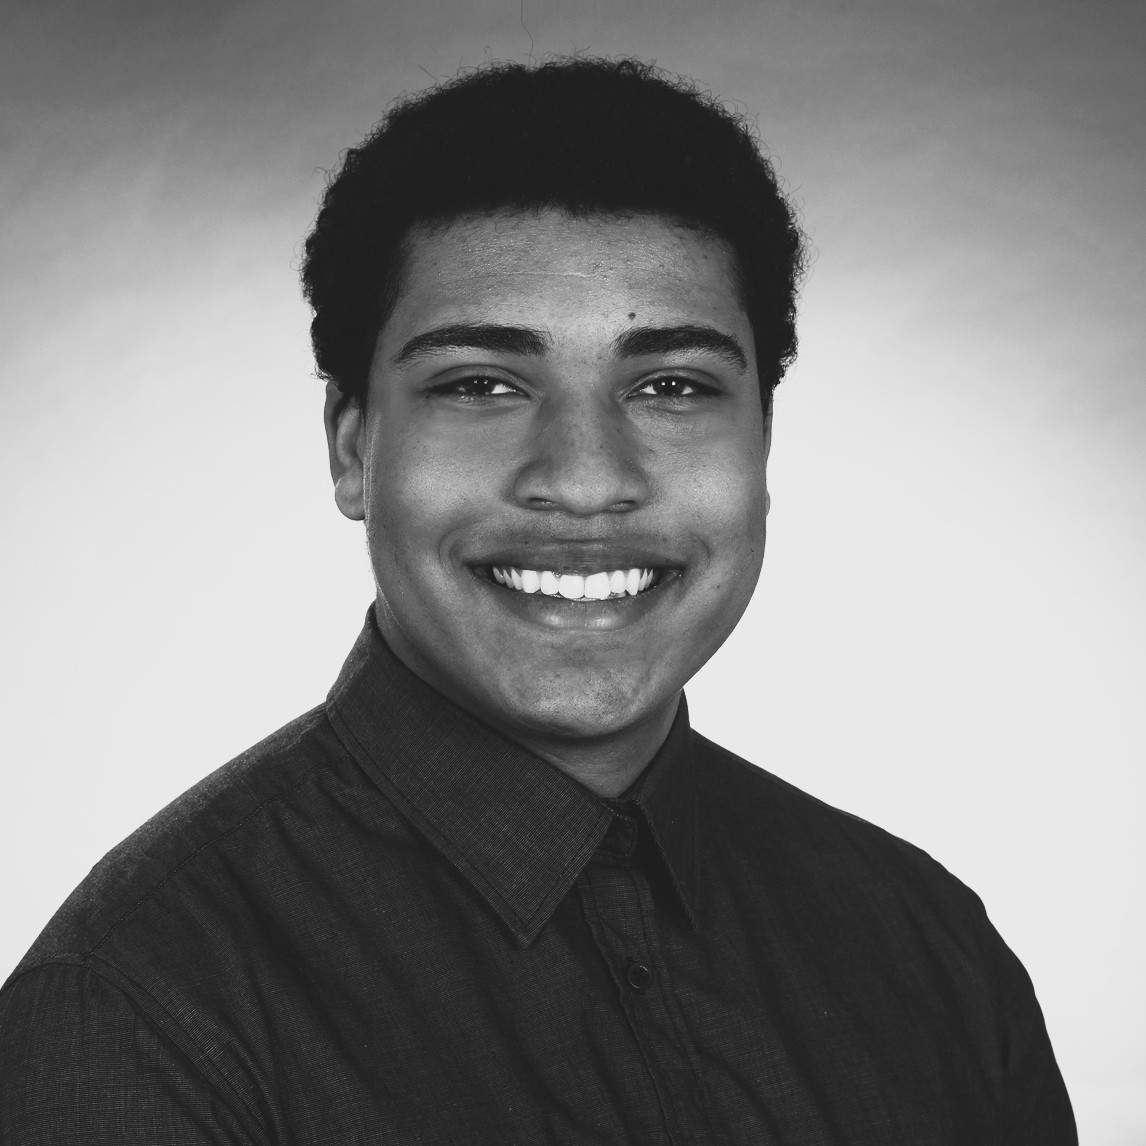
\includegraphics[width=1in,height=1.25in,clip,keepaspectratio]{Figures/Bewerbungsfoto_Ermisch.jpg}}]{Patrick S. Ermisch}
Patrick S. Ermisch was born in Frankfurt am Main, Germany, on December 18, 2002.
He received the Abitur degree and 
is currently pursuing the B.Eng. degree in mechatronics at Frankfurt University of Applied Sciences,
Frankfurt, 
Germany, with an expected graduation in 2026. His major field of study is mechatronics.

He has gained practical experience through an internship at SEW-EURODRIVE, where he contributed to
the further 
development of a mobile application for the manual control of logistics robots. In addition,
he worked as a tutor 
for Physics~I and Physics~II and as a student research assistant, supporting research on particle
simulation and 
the development of an application for visualization and simulation purposes. His research interests include 
reinforcement learning for robotics, space robotic systems, and simulation-based control methods.

Mr.\ Ermisch has been listed on the Dean’s List of Frankfurt University of Applied Sciences
multiple times in 
recognition of his academic performance.
\end{IEEEbiography}



\begin{IEEEbiography}[{
\includegraphics[width=1in,height=1.25in,clip,keepaspectratio]{Figures/egk.jpg}}]{Eric Guiffo Kaigom} was born in Douala, Cameroon. He received the Dipl.-Ing. and \mbox{Dr.-Ing.}
(summa cum laude) degrees in electrical engineering from RWTH Aachen University,  Germany. He was
a Research Associate with the Institute for Man-Machine Interaction at RWTH Aachen University, where
he led the ``Intelligent Robots'' team and coordinated technology development and transfer activities with
partners in robotics-based manufacturing and on-orbit servicing, including projects funded under the European Union's
Horizon 2020 and In-Space Automation programs. He then worked in industry as Head of
Emerging Technologies. Dr. Kaigom is currently a Full Professor with Frankfurt University of Applied
Sciences, Germany. He serves the academic community as an Associate Editor. His current research
interests include robotics, digital twins, agentic systems, and AI $\slash$ ML.
\end{IEEEbiography}

\EOD

% Collect the leftover vertical space of the final (under-full) column here,
% below the end-of-document mark. Each IEEEbiography starts with a "plus 1fil"
% spacer; on a short last page \flushbottom stretches those, spreading the two
% biographies apart. This second-order "fill" out-stretches those first-order
% "fil" spacers, so the slack pools at the bottom and the biographies stay
% close together. The trailing \null anchors the glue so it is not discarded.
\vskip 0pt plus 1fill\relax
\null

\end{document}
